\documentclass[twoside,twocolumn]{article}
\usepackage{acta}
\usepackage{url}
\usepackage[utf8]{inputenc}
\usepackage{setspace}
\usepackage{graphicx}
\usepackage{subfig}
\usepackage{caption}
\usepackage{sectsty}

\allsectionsfont{\bfseries}

\newtheorem{mydef}{Définition}

\begin{document}
\Eingang{00}{00}{0000} \Annahme{00}{00}{0000} \Sachgebiet{1}
\PACS{43.50.Lj, 43.50.Rq, 43.50.Qp, 43.66.Lj, 43.66.Ba}
\Band{0} \Jahr{0000} \Heft{} \Ersteseite{1} \Letzteseite{}

\AuthorsI{G. Lafay$^{1)}$, M. Rossignol$^{2)}$, N. Misdariis$^{2)}$, M. Lagrange$^{1)}$, J.F. Petiot$^{1)}$}
\AddressI{$^{1)}$ Institut de Recherche en Communications et  Cybern\'etique de Nantes (IRCCYN), Nantes, France.\\
\hspace*{8pt}gregoire.lafay@irccyn.ec-nantes.fr\\
$^{2)}$ STMS Ircam-CNRS-UPMC Institut de Recherche et Coordination Acoustique/Musique, Paris, France}

\newcommand{\gl}[1]{\textcolor{blue}{GL : #1}}
\newcommand{\jlv}[1]{\textcolor{magenta}{#1}}
\newcommand{\jls}[1]{\textcolor{red}{#1}}
\newcommand{\jlc}[1]{\textcolor{green}{#1}}

\newcommand{\ie}{\emph{i.\,e.}}
\newcommand{\Ie}{\emph{I.\,e.}}
\newcommand{\cf}{cf.}
\newcommand{\Cf}{Cf.}
\newcommand{\vs}{\emph{vs.}}
\newcommand{\Vs}{\emph{Vs.}}
\newcommand{\al}{\emph{et~al.}}
\newcommand{\eg}{\emph{e.\,g.}}
\newcommand{\Eg}{\emph{E.\,g.}}
\newcommand{\etc}{\emph{etc.}}
\newcommand{\myfloatalign}{\centering}

\Englishtitle{Investigating soundscapes perception through acoustic scenes simulation.} \Germanorfrenchtitle{}

\Kolumnentitel{Lafay et al. : Approaching mental representations}

\Englishabstract{This paper introduces a new experimental protocol to study mental representations of urban soundscapes through a simulation process. Subjects are asked to create a full soundscape by means of a  software dedicated to sound edition, coupled with a structured sound data set. This paradigm is used to characterize urban sound environment representations by analyzing the sound classes that were used to simulate the auditory scenes. A rating experiment of the soundscape pleasantness using a 7-points bipolar scale is conducted to further refine the analysis of the simulated urban acoustic scenes. Results show that 1) a semantic characterization in terms of presence~/ absence of sound sources is an effective way to characterize urban soundscapes pleasantness, and 2) physical descriptors computed for specific sound sources better characterize the appraisal than global descriptors.}
\Germanorfrenchabstract{}

\ScientificPaper



%%%%%%%%%%%%%%%%%%%%%%%%%%%%%%%%%%%%%%%%%%%%%%%%%%%%%%%%%%%%
%%%%%%%%%%%%%%%%%%%%   INTRODUCTION      %%%%%%%%%%%%%%%%%%%
%%%%%%%%%%%%%%%%%%%%%%%%%%%%%%%%%%%%%%%%%%%%%%%%%%%%%%%%%%%%

%\onecolumn
\setlength{\parindent}{5ex}
%\setstretch{2}

\section{Introduction}
\label{sec:intro}

Un des objectifs premiers des études sur les paysages sonores est d'identifier les informations contenues dans l'environnement qui influent sur les sensations perçues \cite{aletta2016soundscape}. Questionner le lien entre sensation (\eg~calme) et environnement (\eg~scène sonore urbaine), revient à objectiver la représentation mentale que se fait un sujet d'une scène sonore en particulier (\eg~une scène sonore urbaine calme).

Si on demande à un sujet d'évaluer un environnement donné suivant une échelle perceptive donnée (\eg~calme, agrément) \cite{axelsson2005soundscape,davies2013perception,cain2013development}, le gain d'information est conditionné par la nature des stimuli disponibles, qu'il s'agisse de scènes sonores enregistrées (expérience en laboratoire), ou réelles (expérience \emph{in situ}). Cependant, le fait que ces stimuli existent permet d'en établir une description physique précise.

Si, à l'inverse, on demande à un sujet de décrire un environnement donné (\eg~décrivez une scène sonore urbaine «~calme~») \cite{guastavino2006ideal, dubois2006cognitive}, on collecte une information riche, symbolique et sémantique, de la représentation qu'il se fait de cet environnement. Néanmoins, en l'absence de données sonores, on ne peut la caractériser physiquement.

Nous pensons que la simulation permet de faire un lien élégant entre ces deux approches. Demander au sujet de simuler un environnement sonore donné revient à obtenir de lui une version modale, \ie~établie sur des dimensions physiques (le signal de la scène simulée), de sa représentation mentale de l'objet, des scènes caractérisées à la fois sémantiquement (\eg~sources sonores présentes) et physiquement (\eg~niveaux des sources sonores).

De plus en plus de travaux tendent à montrer que toutes les sources ne participent pas de manière égale à la perception de la scène sonore \cite{defreville2004aactivity,lavandier2006contribution,guastavino2006ideal,nilsson2007soundscape,
szeremeta2009analysis}. Les recherches portent désormais sur l'étude des contributions spécifiques des différentes sources sur les qualités affectives de la scène \cite{gozalo2015relationship,ricciardi2015sound}. Ces recherches requièrent des outils permettant d'analyser séparément les influences des éléments sonores qui composent l'environnement.

Nous pensons que ces efforts de recherche peuvent grandement bénéficier de l'utilisation de scènes simulées, scènes dont les caractéristiques structurelles, en particulier la nature des sources présentes, leur répartition temporelle ainsi que leur forme d'onde respectives, sont directement accessibles par l'expérimentateur.

Afin de répondre à ces problématiques, nous proposons d'utiliser un outil de simulation permettant à un sujet de simuler des paysages sonores à partir d'un corpus de sons enregistrés. Pour montrer l'intérêt de l'utilisation d'un tel outil pour questionnner la perception de l'environnement sonore, nous choisissons, comme cadre applicatif, le problème de l'agrément perçu dans les environnements sonores urbains. Nous présentons les résultats d'une série d'expériences s'appuyant sur la simulation, et visant, chacune, à comprendre comment les différentes sources sonores qui composent une scène influent sur la perception de l'agrément:

\begin{enumerate}
\item \emph{expérience 1.a, simulation}:  les sujets simulent les environnements qui serviront de stimuli pour les étapes suivantes;
\item \emph{expérience 1.b, évaluation de l'agrément}: les sujets doivent évaluer l'agrément des scènes simulées à partir d'une échelle sémantique;
\item \emph{expérience 2, évaluation de l'agrément après modification des scènes}: comme pour l'expérience précédente, les sujets doivent évaluer l'agrément des scènes simulées à partir d'une échelle sémantique. Cependant les scènes ont été modifiées, \ie~privées de certaines classes de sons identifiées comme ayant un impact sur l'agrément perçu.
\end{enumerate}

A notre connaissance, seuls Bruce~\al \cite{bruce2009development,bruce2014effects} se sont servis de la simulation dans une apporche similaire. Ils proposent un outil permettant d'agir sur un environnement en ajoutant ou supprimant des sources sonores spécifiques d'une part, en modifiant le niveau sonore des sources, et leurs positions spatiales d'autre part. Leurs sujets recréent un un environnement urbain en manipulant un jeu de sources sonores pré-établies. Les auteurs montrent que l'inclusion ou l'exclusion des sources dépendent plus de considérations sociales/sémantiques, que de leurs caractéristiques physiques. Ils soulignent néanmoins que le manque d'enregistrements disponibles limite l'analyse.

Dans notre démarche, le simulateur utilisé \foonote{simScene, disponible en ligne \url{http://soundthings.org/research/}} permet une restitution simplifiée (monophonique) des scènes, au profit d'un nombre plus important de paramètres et de sources disponibles, ce afin de garantir, à la sortie, des données viables et expressives.

Le papier comprend 5 sections: Introduction, L'outil de simulation \emph{SimScene}, Expérience 1 .a \emph{simulation} et .b \emph{évaluation de l'agrément}, Expérience 2 \emph{évaluation de l'agrément après modification des scènes}, et Conclusions et perspectives.

Dans le cadre de cette communication, nous ne présentons de \emph{SimScene} que les fonctionnalités pertienentes pour notre étude. Pour plus de détails, se référer à \cite{rossignol2015simscene,lafay2016JAES}. L'expérience 1 .a a fait l'objet d'une étude pilote dont les résultats sont présentés dans \cite{lafay2013atiam,lafay2014new}.

%%%%%%%%%%%%%%%%%%%%%%%%%%%%%%%%%%%%%%%%%%%%%%%%%%%%%%%%%%%%
%%%%%%%%%%%%%%%%%%%%   SIMSCENE      %%%%%%%%%%%%%%%%%%%%%%%
%%%%%%%%%%%%%%%%%%%%%%%%%%%%%%%%%%%%%%%%%%%%%%%%%%%%%%%%%%%%


\section{L'outil de simulation}
\label{sec:simscene}

\emph{Simscene} est un environnement de travail audio-numérique dont la première version a été développée dans le cadre du projet HOULE\footnote{\emph{Projet HOULE} : \url{houle.ircam.fr}}. Il est prévu pour fonctionner sur les navigateurs internet \emph{Chrome} et \emph{Firefox}. L'outil a été développé en javascript à l'aide de la bibliothèque \emph{angular.js}\footnote{\emph{angular.js} : \url{angularjs.org}} et du standard \emph{web-audio}\footnote{\emph{web-audio} : \url{www.w3.org/TR/webaudio}}. L'interface de sélection (\cf~Section~\ref{sec:simscene_ssf}) a été développée à l'aide de la bibliothèque \emph{D3.js} \cite{d32011}.

Le fonctionnement de \emph{Simscene} se rapproche de celui d'un séquenceur audio. Chaque utilisateur choisit une classe de sons via l'interface de sélection (\cf~Section~\ref{sec:simscene_ssf}). Une fois la classe de sons sélectionnée, une piste audio, liée à cette classe, est créée. L'utilisateur peut alors modifier certaines propriétés de la piste via un groupe de paramètres de contrôle propre à chacune (\cf~Section~\ref{sec:simscene_parametre}). Des champs de texte sont prévus afin de permettre à l'utilisateur 1) de nommer chaque piste, 2) de donner un titre à la scène simulée 3) de commenter la scène simulée.

\subsection{Banque de données de samples}
\label{sec:simscene_sampleDataSet}

\subsubsection*{Typologie}

Afin de créer un corpus de classes de sons de référence pour la simulation, nous réalisons une typologie des sons environnementaux urbains.

Une étude bibliographique est effectuée, afin d'identifier les sources et ambiances sonores les plus souvent citées dans les publications. Cette étude porte sur 16 articles ou thèses \cite{maffiolo_caracterisation_1999,raimbault2002simulation,guastavino_etude_2003,defreville2004aactivity,raimbault2005urban,dubois2006cognitive,devergie_relations_2006,guastavino2006ideal,niessen2010categories,maffiolo_caracterisation_1999,beaumont2004pertinence,polack2008perceptive,leobon_analyse_1986,brown2011towards}
traitant de la manière dont nous discriminons les paysages sonores urbains. Notre typologie est établie sur la base des catégories/classes de sons relevées dans cette littérature.

Les réactions à la musique étant jugées trop subjectives, et les jugements esthétiques ne pouvant qu'altérer les données d'évaluation, nous choisissons, dans cette étude, de ne pas considérer les sources musicales de type musiciens de rue, radios de voitures, d'appartements, \etc.

\subsubsection*{Événements et Textures}

La littérature fait généralement la distinction entre :

\begin{itemize}
\item {un événement sonore}: un son isolé, ponctuel, dont les caractéristiques physiques varient au cours du temps;
\item {une texture sonore}: un son, isolé, long, dont les caractéristiques physiques restent stables au cours du temps \cite{saint1995classification}.
\end{itemize}

L'outil de simulation \emph{Simscene} tient compte de cette distinction, et utilise deux banques de données distinctes : l'une regroupant classes d’événements, l'autre des classes de textures. Événements et textures bénéficient de processus de simulation particuliers.

Les différences morphologiques entre événements et textures sonores ont des conséquences sur la perception des scènes.

Lorsque des événements émergent d'un environnement sonore, le cerveau traite l'information des différentes sources de manière séparée. Plusieurs flux auditifs sont ainsi générés, \ie~un pour chaque séquence d'événements émis par la même source \cite{carlyon2004brain}. Inversement, quand le cerveau ne parvient pas à isoler d'événements, les éléments constituants de la scène sont agglomérés dans un même flux.

Maffiolo \cite{maffiolo_caracterisation_1999} met en évidence deux processus de catégorisation distincts, engagés en fonction de la capacité de l'auditeur à identifier des événements sonores. Elle montre l'existence de deux catégories cognitives abstraites d'environnements sonores respectivement appelées: «~les séquences événementielles~» et «~les séquences amorphes~».

Les séquences événementielles sont des environnements composés d'événements saillants et identifiables (\emph{démarrage de voiture}, \emph{voix d'homme}). Elles profitent d'une analyse descriptive basée sur l'identification des sources sonores. Les séquences amorphes sont des environnements dont il est difficile d'isoler des éléments distincts («~brouhaha de rue~», «~brouhaha de trafic~»). Elles profitent, elles, d'une analyse holistique, effectuée à partir d'indicateurs acoustiques (subjectifs) globaux. Cette différence de traitement entre scènes événementielles et scènes amorphes est relevée également dans \cite{guastavino2006ideal,dubois2006cognitive}.

Pour ce qui est des textures, \ie~des sons possédants des caractéristiques stables au cours du temps, \cite{mcdermott2011sound,mcdermott2013summary} montrent que le cerveau peut décider sciemment de dégrader l'information physique perçue, en la résumant de manière statistique, faisant fi de toute autre représentation plus détaillée \cite{nelken2013ear}.

Au regard de ces résultats, il apparaît que le processus de traitement de l'information sonore comprend une prise de décision quant à la nature des stimuli \cite{nelken2013ear,mcdermott2013summary}, laquelle va ensuite influer sur la manière d'extraire et d'analyser l'information.

\subsubsection*{Taxonomie}

\begin{figure}[t]
        \myfloatalign
        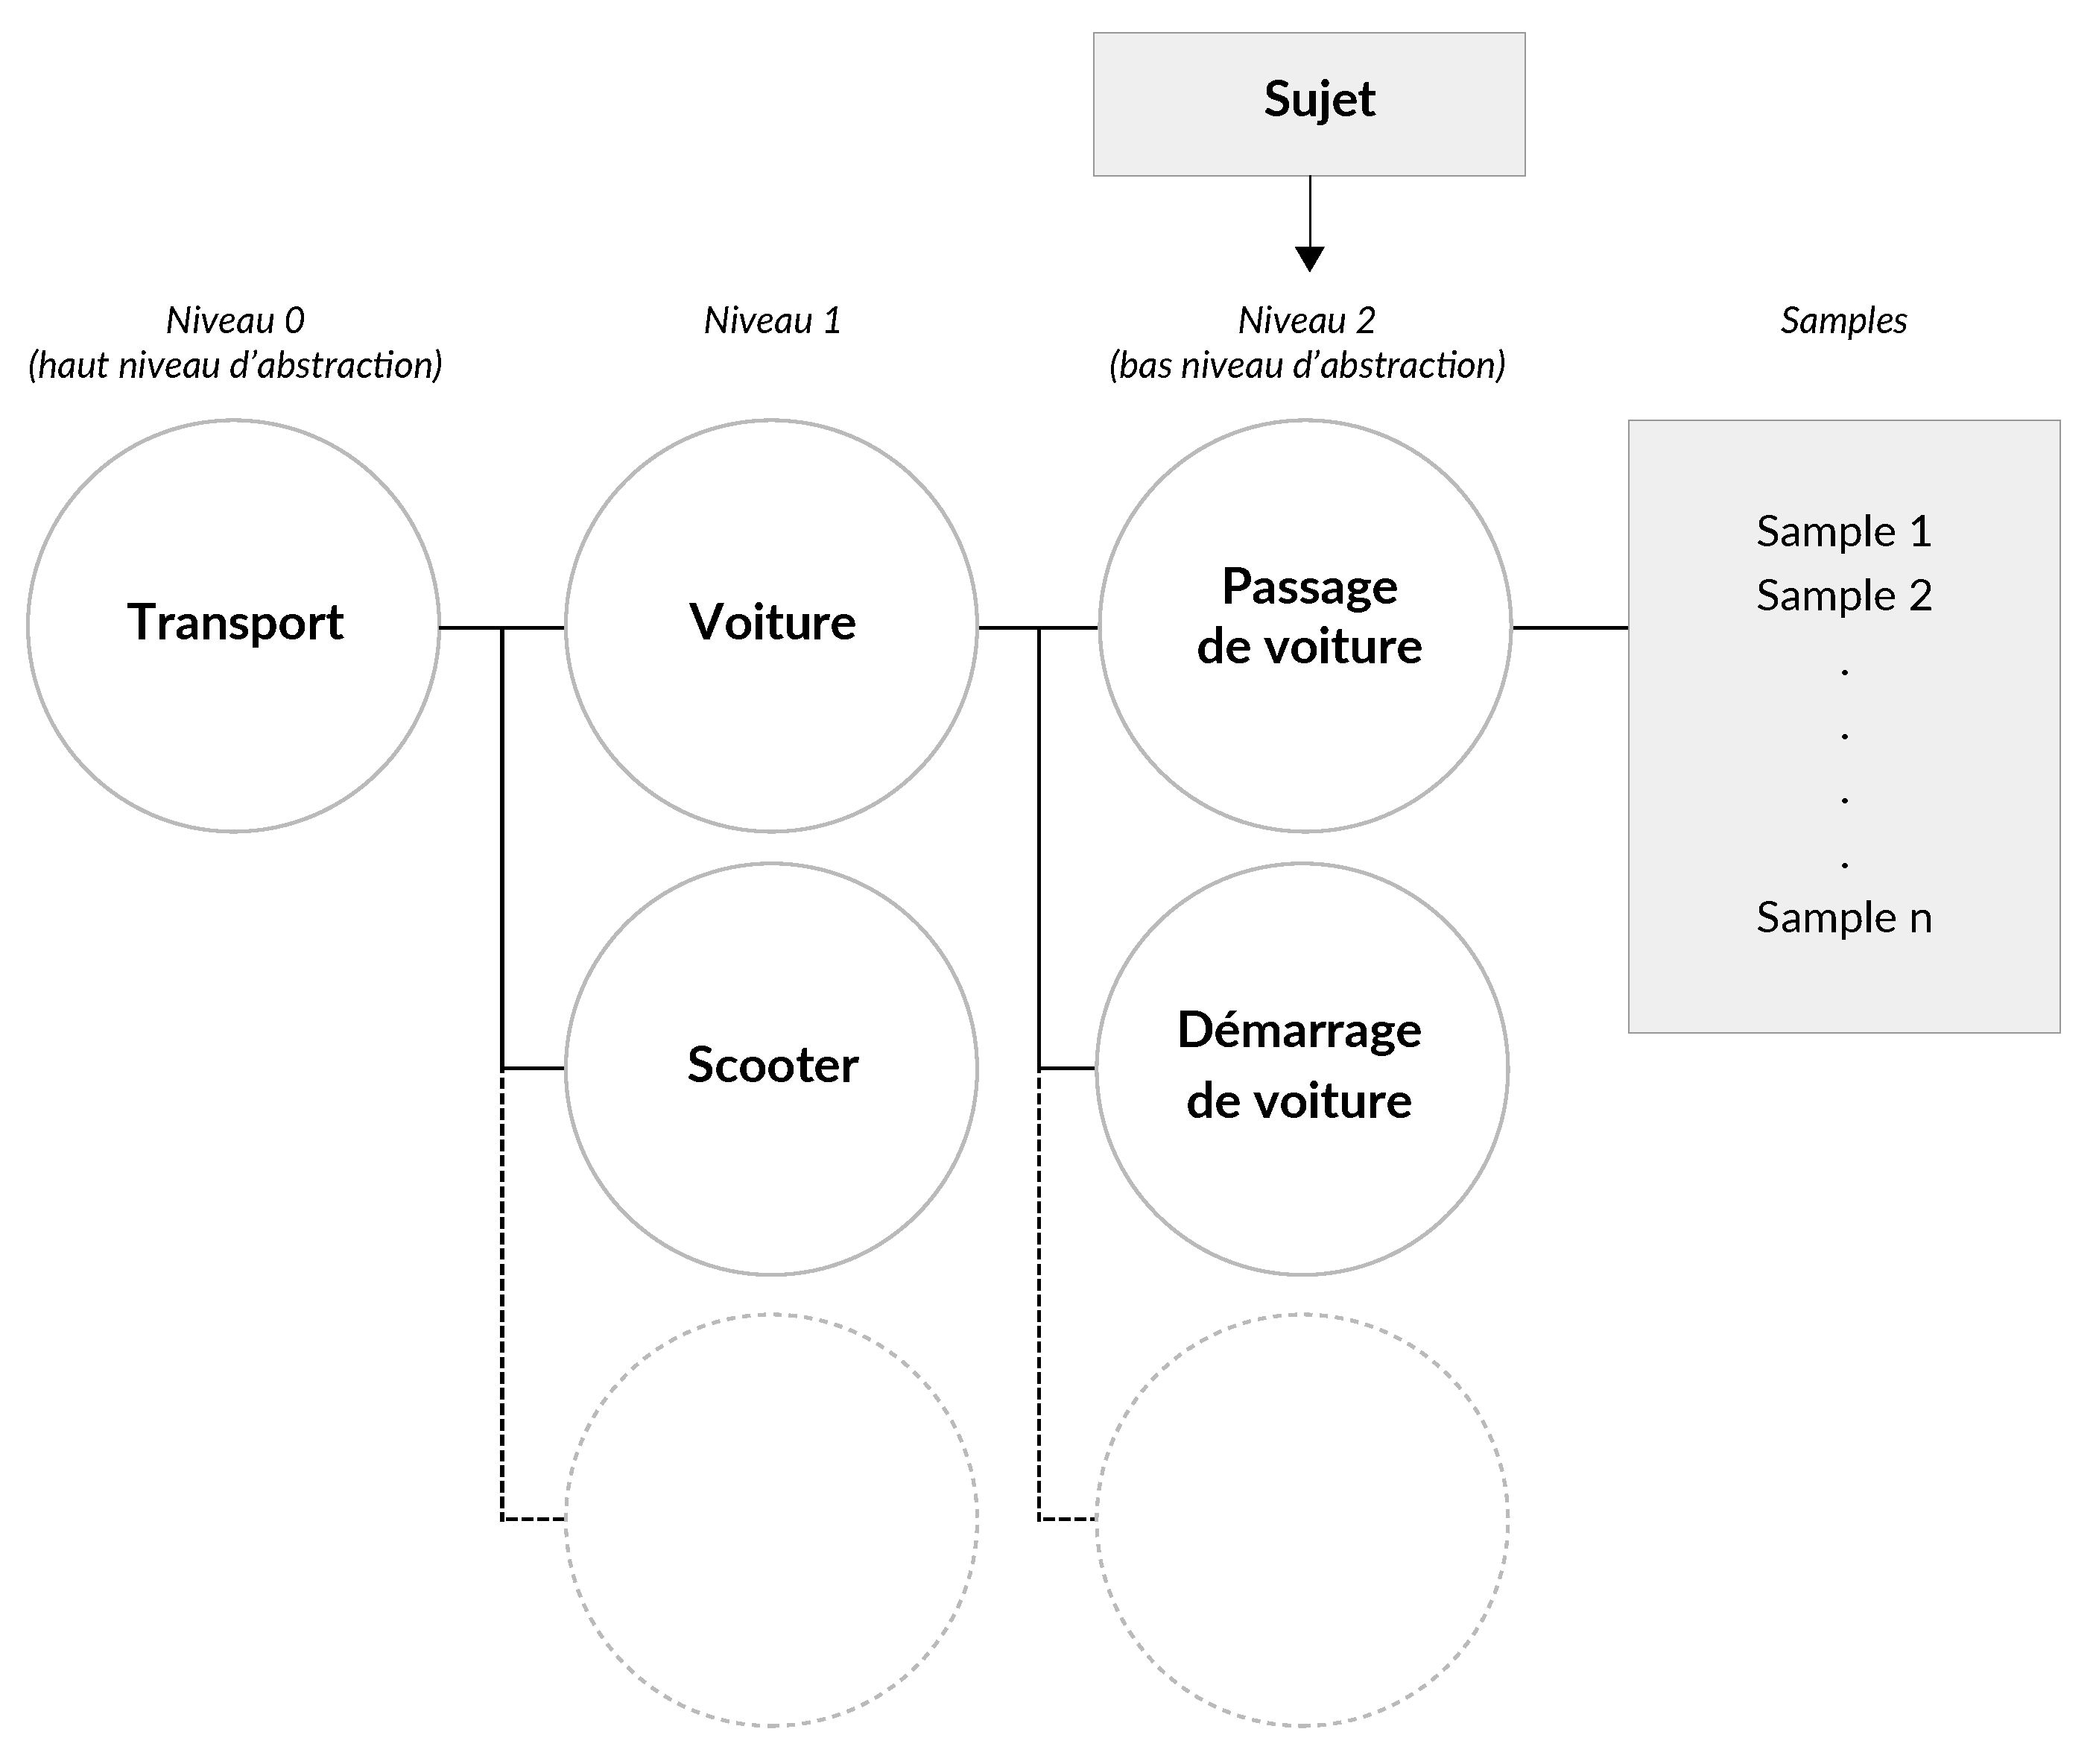
\includegraphics[width=.8\linewidth]{gfx/ch_4/3}
       \caption{Organisation hiérarchique de la banque de sons isolés utilisée pour la simulation.}\label{fig:orgDb}
\end{figure}


Nous nommons sample, un enregistrement d'un son isolé, événement ou texture. Chaque classe est alors comprise comme une collection de samples jugés perceptivement équivalents.

Les classes de sons sont organisées suivant une structure hiérarchique (\cf~Figure~\ref{fig:orgDb}). Cette structure hiérarchique est largement inspirée de l'axe vertical de l'organisation catégorielle proposée par E. Rosch \cite{rosch1978cognition}, qui dresse une taxonomie des classes ou catégories \ie~plus le niveau d'abstraction de la classe est faible, plus la description de la classe est précise, et plus les sources sonores incluses dans cette classe sont semblables. Si le niveau d'abstraction d'une classe est tel que cette dernière possède des sous-classes, alors sa collection de samples est la somme des collections respectives de chacune des sous-classes.

Nous établissons deux taxonomies, une pour les événements, une autre pour les textures (\cf~Annexe~\ref{app:taxonomie}). Pour les événements, nous considérons quatre niveaux d'abstraction allant des classes les plus globalisantes (niveau d'abstraction 0), aux classes les plus spécifiques (niveau d'abstraction 3). Pour les textures, nous ne considérons que trois niveaux d'abstraction. Notons que la taxonomie des événements est proche de celle de \cite{Salamon14}, introduite postérieurement à notre étude.

\subsubsection*{Acquisition des samples}

Sur la base des taxonomies précédemment établies, 483 sons isolés ont été collectés, dont 381 événements, et 102 textures. Parmi ces samples, 332 ont été enregistrés, et 151 proviennent de différentes banques de sons (\emph{SoundIdeas}\footnote{\emph{SoundIdeas}: \url{www.sound-ideas.com}} et \emph{Universal SoundBank}\footnote{\emph{Universal SoundBank}: \url{www.universal-soundbank.com}}).

Tous les enregistrements ont été effectués à l’aide d'un micro canon \emph{AT8035}\footnote{\emph{Micro canon AT8035}: \url{eu.audio-technica.com}} relié à un enregistreur \emph{ZOOM H4n}\footnote{\emph{ZOOM H4n} : \url{www.zoom.co.jp/english/products/h4n}}. L’utilisation du micro canon nous permet d’isoler les événements sonores du brouhaha urbain. Pour les textures, il nous permet d’éviter les événements sonores proches du preneur de son. Nous pouvons ainsi pointer des "zones sonores", en nous tenant à une certaine distance de ces dernières, afin de capter uniquement le brouhaha émanant de la zone ciblée.

Tous les sons ont été normalisés au même niveau $RMS$ de $-12$ $dB$ (FS), \ie. relativement à un niveau pleine échelle (\emph{relative to Full Scale}). Dans notre cas, ce niveau pleine échelle est de 1 Volt.

\subsection{Paramètres}
\label{sec:simscene_parametre}

Par choix de conception, l'outil de simulation ne permet pas d’interagir avec un sample en particulier, mais toujours avec une piste, \ie~une séquence de samples. Plusieurs paramètres permettent au sujet de contrôler la structure de chaque piste.

\begin{itemize}
\item \emph{niveau sonore} ($dB$): pour chaque sample, les niveaux sont tirés aléatoirement à partir d'une distribution normale, paramétrée par le sujet en terme de moyenne et de variance;
\item \emph{espacement inter-onset} (seconde): (piste d'événements seulement) comme pour les niveaux, les espacements sont tirés aléatoirement à partir d'une distribution normale, paramétrée par le sujet en terme de moyenne et de variance;
\item \emph{début et fin} (seconde): le sujet fixe le début et la fin de chaque piste.
\end{itemize}

Afin de faciliter la simulation, deux paramètres supplémentaires sont proposés:

\begin{itemize}
\item \emph{fondu par événement} (seconde): (piste d'événements seulement) le sujet fixe une durée de fondu (entrée et sortie) appliquée à chaque sample;
\item \emph{fondu global} (seconde): le sujet fixe les durées de fondus pour l'entrée et la sortie de la piste. Ces fondus s'appliquent ainsi à l'ensemble des samples de la piste.
\end{itemize}

Deux de ces paramètres ne s’appliquent que pour les pistes d'événements (\emph{fondu par événement}  et \emph{espacement inter-onset}), les samples des textures étant séquencés sans espacement.

\subsection{Interface de sélection}
\label{sec:simscene_ssf}

La grande majorité des outils permettant de parcourir une banque de données propose une recherche textuelle sur la base de mots clefs. Dans le cadre d'une expérience sensorielle visant à objectiver la représentation interne du sujet, cette approche est problématique.

En effet la description verbale du son, si elle est accessible au sujet, peut potentiellement influencer sa sélection. Dans les faits, pour construire une scène environnementale «~calme~», le sujet sélectionne a priori les sons référencés sous le vocable \emph{parc}.

Pour limiter l’influence de l’interface sur le sujet, il nous paraît nécessaire de libérer sa recherche de toute information textuelle. Nous proposons à l'utilisateur une interface graphique lui permettant d’explorer la banque de sons exclusivement à partir de l’écoute.

La figure~\ref{fig:ssf} présente l'interface pour la banque de données d'événements sonores. Visuellement, les classes du dernier palier (niveaux d'abstraction 3 pour les événements, 2 pour les textures) sont représentées par des cercles, et positionnées sur un plan. La disposition des cercles dans l'espace dépend de l’organisation hiérarchique de la base de données: les sous-classes appartenant à une même classe sont proches les unes des autres, et ainsi de suite jusqu'à atteindre les classes du dernier palier, les seules auxquelles le sujet peut accéder, des classes qui ne possèdent pas de sous-classes, et sont directement liées à une collection de samples.

Chaque classe du dernier palier possède un son prototype. Ces sons ont été choisis par les expérimentateurs. Lorsqu’on clique sur un cercle, le prototype associé à la classe est joué. Le sujet parcourt la banque de sons en cliquant sur les cercles.

Cette interface a fait l'objet d'une étude approfondie dont les résultats sont publiés dans \cite{lafay2016JAES}.

\begin{figure}[t]
        \myfloatalign
        \subfloat[]
        {\includegraphics[width=.8\columnwidth]{gfx/ch_4/SSF}\label{fig:ssf}} \par
        \subfloat[]
        {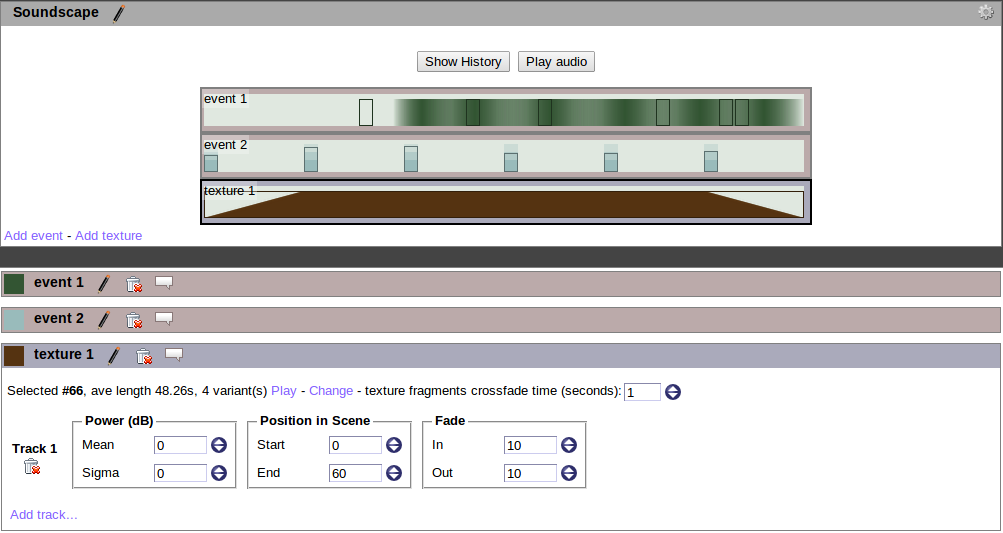
\includegraphics[width=\columnwidth]{gfx/ch_4/simscene}\label{fig:simscene}}
       \caption{Les interfaces de sélection (a) et de simulation (b) de l'outil \emph{Simscene}.}
\end{figure}

\subsection{Interface de simulation}

L'interface de simulation propose un rendu graphique schématisé de la scène en cours de création (\cf~Figure~\ref{fig:simscene}). La piste est représentée par une bande possédant un axe temporel. Sur cette bande, chaque sample est représenté par un rectangle. L'espacement entre les rectangles est fonction de l'espacement entre les samples. De même, la hauteur des rectangles est proportionnelle au niveau sonore des samples. Dans le cas d'une piste de texture, un unique rectangle apparaît sur toute la longueur de la piste, un son de texture ne pouvant être entrecoupé de silences. Les caractéristiques des rectangles évoluent en fonction des changements de paramètres de la piste. L'utilisateur a la possibilité, à tout moment, d'écouter la scène simulée.

La scène sonore est ainsi vue comme une somme de sources sonores, ou, si l'on admet la distinction opérée entre événements et textures sonores, «~un squelette d'événements sur un lit de textures~» \cite{nelken2013ear}. Cet outil de simulation est présenté en détail dans \cite{rossignol2015simscene}.

%%%%%%%%%%%%%%%%%%%%%%%%%%%%%%%%%%%%%%%%%%%%%%%%%%%%%%%%%%%%
%%%%%%%%%%%%%%%%%%%  Experience 1     %%%%%%%%%%%%%%%%%%%%%%
%%%%%%%%%%%%%%%%%%%%%%%%%%%%%%%%%%%%%%%%%%%%%%%%%%%%%%%%%%%%

\section{Expérience 1}
\label{sec:xp1}

\subsection{Objectif}

L'objectif est d'étudier les influences spécifiques des différentes sources sonores qui composent les environnements urbains sur la perception de l'agrément, en utilisant la simulation. Pour ce faire, nous planifions nos deux premières expériences (\cf~Figure~\ref{fig:xp1_2}):

\begin{itemize}
\item \emph{expérience 1.a de simulation}: au cours de cette expérience, les sujets doivent simuler des environnements sonores urbains, en utilisant l'outil de simulation \emph{Simscene} (\cf~Section~\ref{sec:simscene}). Chacun compose deux environnements sonores, le premier idéal/agréable et le deuxième non-idéal/désagréable.

\item \emph{expérience 1.b d'évaluation}: à l'issue de la simulation, nous n'avons, de fait, qu'une connaissance binaire des propriétés affectives des scènes simulées: idéale (i) et non-idéale (ni). Cette seconde étape a pour but d'affiner notre connaissance sur l'agrément. Pour ce faire, nous demandons à un deuxième groupe de sujets d'évaluer, à partir d'une échelle sémantique, l'agrément de chacune des scènes simulées. L'expérience d'évaluation sert deux buts:

\begin{enumerate}
\item évaluer l'influence respective des différentes sources sur l'agrément, pour chaque type d'environnement (i ou ni);
\item détecter la présence de cas extrêmes ou ambigus (\emph{outlier}) dans les scènes simulées. Pour le reste de notre étude, les qualités hédoniques imposées (i et ni) servent de référence, de vérité terrain. Il nous faut donc garantir qu'il n'y ait pas d’ambiguïté entre les cas extrêmes des i- et ni-scènes, \ie~que la note d'agrément la plus basse des i-scènes reste supérieure à la note la plus haute des ni-scènes.
\end{enumerate}

\end{itemize}

Notre analyse s'appuie sur les données produites par les deux expériences.

\begin{figure}[t]
        \myfloatalign
        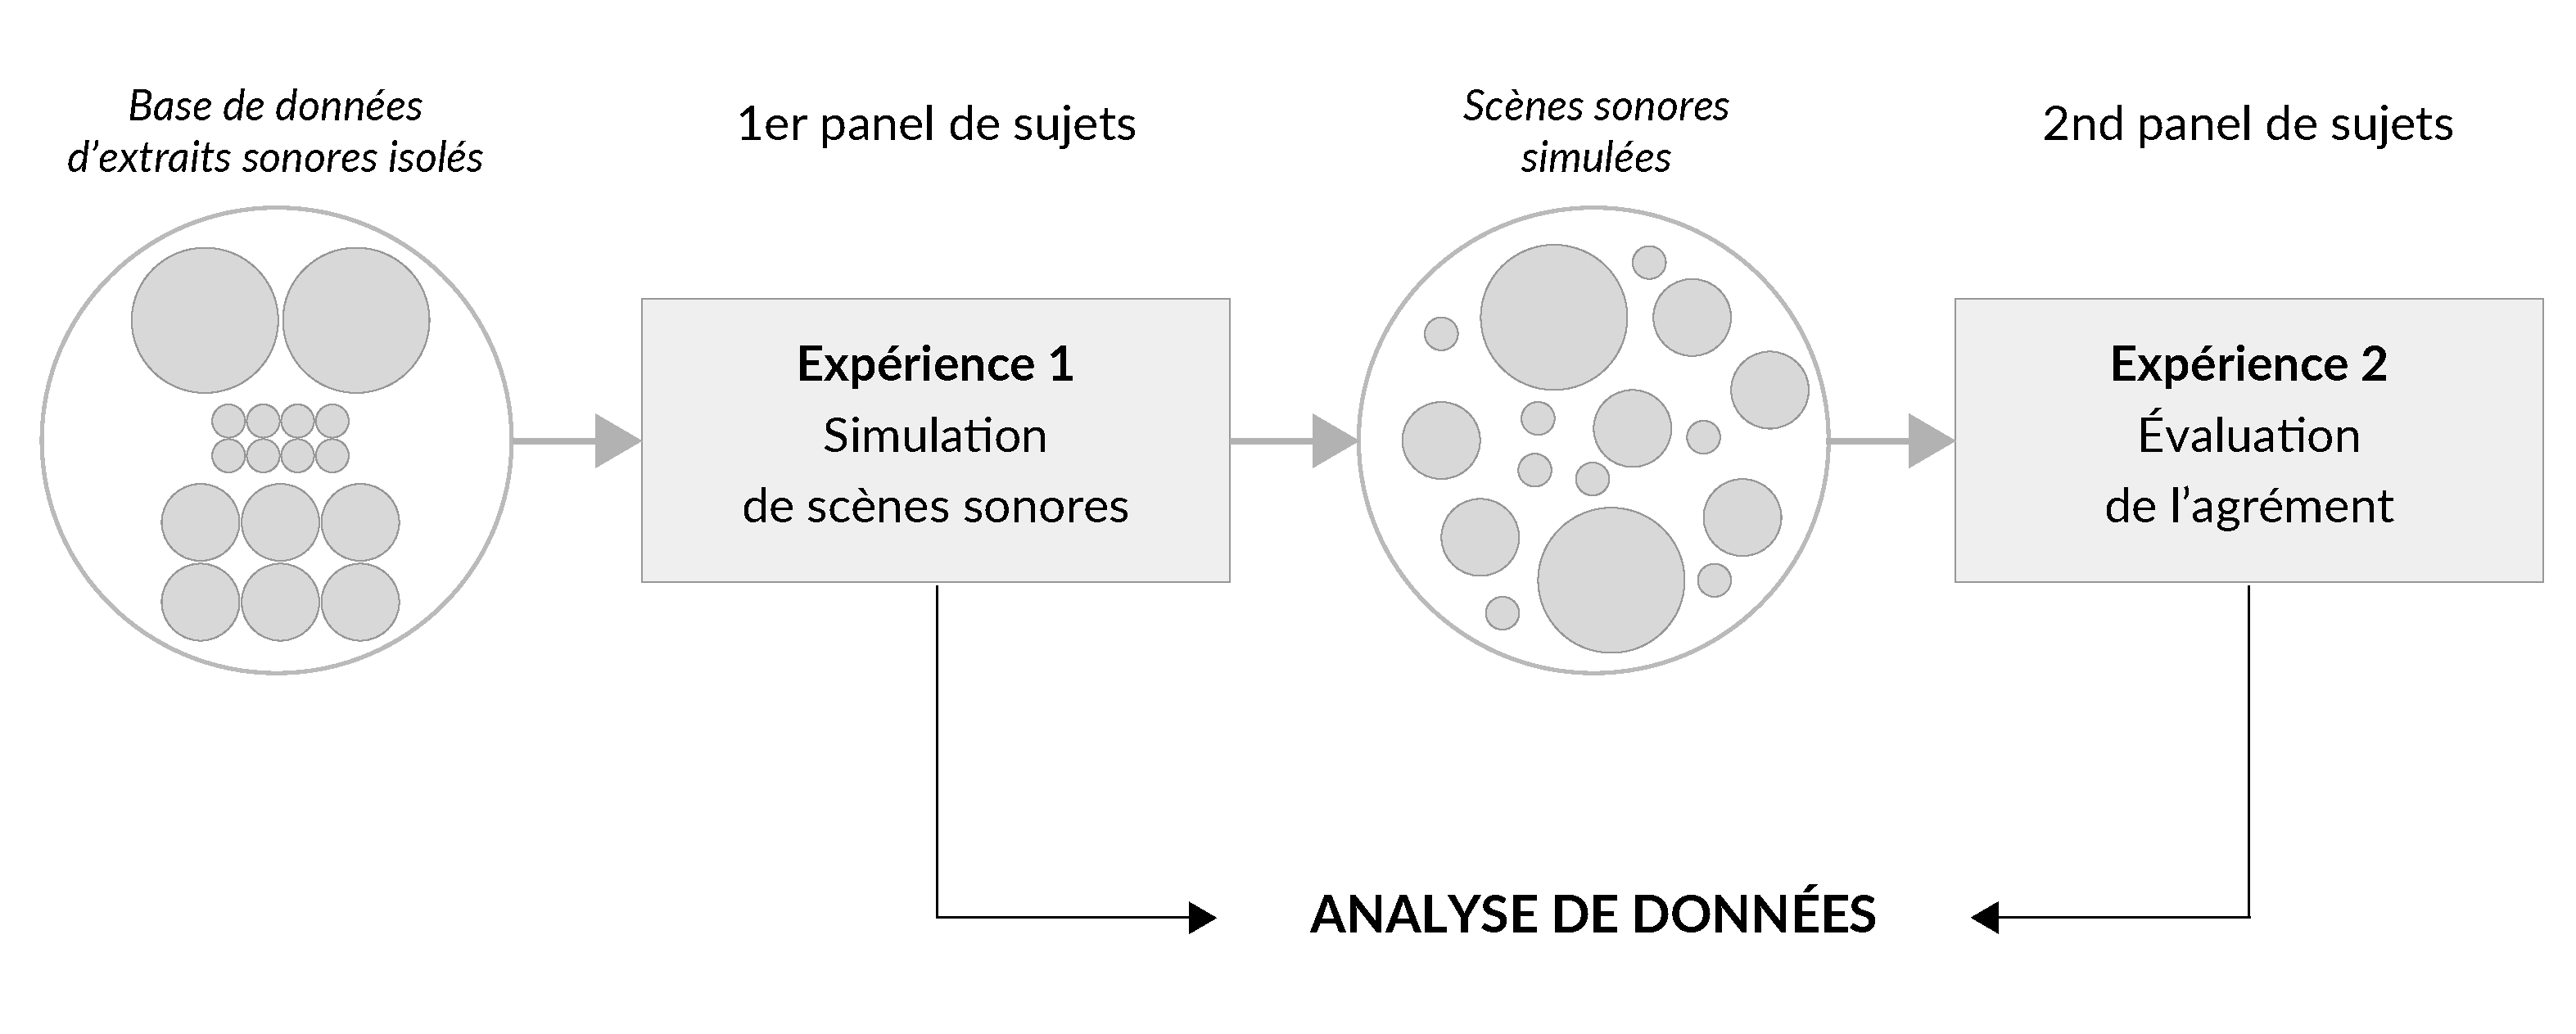
\includegraphics[width=\linewidth]{gfx/ch_5/5}
        \caption{Planification expérimentale des éxperiences de simulation et d'évaluation de l'agrément}\label{fig:xp1_2}
\end{figure}

\subsection{Planification de l'expérience 1.a}
\label{sec:xp1a_plan}

\subsubsection*{Procédure}

Les sujets doivent simuler deux environnements sonores urbains, chacune des scènes devant durer 1 minute. Ils doivent se conformer aux consignes suivantes:

\begin{itemize}
\item première simulation: simuler un paysage sonore \textbf{urbain plausible} qui, selon vous, est idéal (où vous aimeriez vivre);
\item deuxième simulation: simuler un paysage sonore \textbf{urbain plausible} qui, selon vous, est non-idéal (où vous n'aimeriez pas vivre).
\end{itemize}

Tous commencent par simuler l'environnement idéal. Ils ne prennent connaissance de la deuxième consigne qu'à la fin de la première simulation.

Les sujets sont totalement libres dans le choix des sons, et des paramètres. Ils doivent cependant se soumettre à deux contraintes:

\begin{itemize}
\item le sujet doit prendre le point de vue d’un auditeur fixe;
\item le paysage sonore doit être réaliste, au sens de physiquement plausible. Le sujet peut très bien réunir 10 chiens dans un paysage sonore. Il ne peut en introduire 1 qui aboierait toutes les 10 millisecondes.
\end{itemize}

Ces contraintes font partie de la consigne. Aucun contrôle n'est fait \emph{a priori} dans l'interface de simulation.

Chaque processus de simulation comprend deux parties :

\begin{enumerate}
\item la réalisation de la simulation: cette étape se décompose en trois temps:
\begin{itemize}
\item sélectionner les classes de sons
\item nommer les classes de sons sélectionnées
\item paramétrer les pistes (\cf~Section~\ref{sec:simscene_parametre}) relatives aux classes de sons sélectionnées
\end{itemize}
\item la production d'un commentaire libre du paysage sonore simulé
\end{enumerate}

En complément, et une fois les deux scènes sonores réalisées, les sujets sont invités à:

\begin{itemize}
\item indiquer les sources sonores qu'ils voulaient mettre, mais qu'ils n'ont pas trouvées;
\item commenter l’ergonomie du logiciel de simulation;
\item commenter l’ergonomie de l'interface de sélection.
\end{itemize}

Avant de commencer la première simulation, un tutoriel de 20 minutes est proposé aux sujets, afin qu'ils se familiarisent avec le logiciel de simulation, et la banque de données. L'expérience est prévue pour durer 2h30.

\subsubsection*{Dispositif expérimental}

Tous les sujets passent l'expérience sur des machines identiques. L'audio est diffusé en monophonie, par le biais de casques audio. Pendant le tutoriel, les sujets doivent ajuster le niveau sonore à un volume confortable. Ils ne peuvent le modifier par la suite.

Tous les sujets réalisent l'expérience simultanément. Ils sont répartis de manière égale dans trois pièces identiques, toutes possédant un environnement calme. Ils n'ont pas le droit de s'adresser la parole pendant l'expérience.

Trois expérimentateurs, un dans chaque pièce, sont présents durant la totalité de l'expérience, afin de contrôler le bon déroulement de cette dernière, et de répondre aux éventuelles questions des sujets.

\subsubsection*{Participants}

44 étudiants (14 femmes) de L’École Centrale de Nantes ont participé à l'expérience. Ils ont tous sensiblement le même âge (moyenne: 21.6, écart-type: 2). Tous les sujets sont Nantais, et vivent dans cette ville depuis deux ans ou plus.

Sur les 44 sujets, 40 réalisent l'expérience avec succès, produisant au final 80 scènes sonores simulées, dont 40 scènes idéales, et 40 scènes non idéales. 4 sont éliminés pour non respect ou incompréhension des consignes, d'une part, et dépassement du temps, d'autre part.

\subsection{Planification  de l'expérience 1.b}
\label{sec:xp1b_plan}

\subsubsection*{Procédure}

En raison de contraintes temporelles, les sujets n'évaluent que des séquences de 30 secondes des scènes simulées, chacune de ces séquences commençant à la seconde 15, et finissant à le seconde 45 de la scène d'une durée initiale de 1 minute.

L'évaluation s'effectue sur une échelle sémantique bipolaire de 7 points, allant de -3 (non-idéale/très désagréable) à +3 (idéale/très agréable). Avant de noter une scène, les sujets doivent obligatoirement écouter les 20 premières secondes de cette dernière. Après la notation, ils sont libres de passer à la scène suivante.

Pour chaque sujet, les scènes sont présentées dans un ordre aléatoire. Les 10 premières scènes permettent au sujet de calibrer ses notes. Elles sont obligatoirement composées de 5 scènes idéales, et de 5 scènes non-idéales. Ces 10 premières scènes sont rejouées à la fin de l'expérience, et seules les notes données à la deuxième occurrence sont prises en compte.

L'expérience est prévue pour durer 30 minutes. Les sujets ne connaissent pas la nature des scènes.

\subsubsection*{Dispositif expérimental}

Tous les sujets passent l'expérience sur des machines identiques. L'audio est diffusé en monophonie, par le biais de casques audio semi-ouverts \emph{Beyer-Dynamic DT 990 Pro}. Toutes les scènes sonores ont été re-simulées sur la base des partitions obtenues lors de l'expérience de simulation. Le niveau sonore de sortie est identique pour tous les sujets.

Tous les sujets réalisent l'expérience simultanément, dans un environnement calme. Ils n'ont pas le droit de s'adresser la parole pendant l'expérience.

Un expérimentateur est présent durant la totalité de l'expérience, afin de contrôler le bon déroulement de celle-ci, et de répondre aux éventuelles questions des sujets.

\subsubsection*{Participants}

10 étudiants (2 femmes) de L’École Centrale de Nantes ont participé à l'expérience. Aucun d'entre eux n'a réalisé l'expérience de simulation. Tous les sujets ont sensiblement le même âge (moyenne: 23.1, écart-type: 1.8). Tous les sujets sont Nantais, et vivent dans cette ville depuis deux ans ou plus.

Tous les sujets ont réalisé l'expérience avec succès.

\subsection{Données et méthodes d'analyses}
\label{sec:xp1_dataAna}

A chaque scène est associé un groupe de descripteurs. C'est sur ces descripteurs que nous pratiquons l'analyse. Un résumé de ces derniers, ainsi que des acronymes les désignant, est présenté dans le Tableau~\ref{tab:acronyme}. Afin de rester cohérent avec l’expérience 1.b d'évaluation, les descripteurs ne sont pas calculés sur la durée totale des scènes, mais sur la version réduite de 30 secondes (\cf~Section~\ref{sec:xp1b_plan}).

Pour chaque scène sonore, trois types de descripteurs sont considérés:

\begin{itemize}
\item \emph{perceptif}: il s'agit de l'agrément perçu de la scène simulée, évalué sur une échelle sémantique de 7 points. Nous notons $\mathcal{A}_{scene}$ l'agrément moyen d'une scène, obtenu en moyennant les notes de tous les sujets. De même, nous notons $\mathcal{A}_{sujet}$ l'agrément par sujet, en moyennant l'ensemble des notes de chacun. Compte tenu du faible nombre de sujets, nous faisons le choix, dans cette étude, de ne pas normaliser les notes d'agrément;
\item \emph{sémantique}: il s'agit d'un vecteur booléen noté $S=(x_1,x_2,\ldots,x_n)$, indiquant les classes de sons présentes dans la scène. Chaque point $x$ de ce vecteur correspond à une classe de sons particulière: $x=1$ si la classe est présente dans la scène, et $x=0$ autrement. La dimension $n$ des vecteurs dépend du niveau d'abstraction considéré, \eg~pour le niveau d'abstraction 1, qui comprend $44$ classes de sons, cette dimension sera de $n=44$.
\item \emph{structurel}: il s'agit du \emph{niveau Sonore}. Pour représenter le niveau sonore, nous nous inspirons de la mesure $L_{Aeq}$. Dans notre cas, il s'agit d'un scalaire calculé sur le signal en volts, et non en pression, et donné en décibels, en prenant un référentiel de 1 Volt. Le niveau est obtenu en calculant, toutes les secondes, la moyenne quadratique du signal, et en moyennant sur la durée de la scène. Un filtrage de type A est opéré avant le calcul des moyennes quadratiques. Nous notons $L$, $L(E)$ et $L(T)$ les niveaux calculés en tenant compte respectivement de l'ensemble des samples, des samples d'événements et de textures.
\end{itemize}

Pour évaluer l'impact spécifique des différentes sources sonores sur l'agrément perçu, nous soumettons nos travaux aux 5 tests/études de significativité présentés ci-après:

\begin{itemize}
\item \emph{vérification de l'agrément des scènes simulées}: afin de vérifier que la distinction affective imposée entre les i- et ni-scènes se retrouve au niveau de l'agrément perçu, nous observons s'il existe des différences entre les deux types de scènes au niveau de $\mathcal{A}_{scene}$ et $\mathcal{A}_{sujet}$. La significativité est évaluée par un test de Student à deux populations indépendantes pour $\mathcal{A}_{scene}$, et par un test de Student à deux populations appariées pour $\mathcal{A}_{sujet}$;
\item \emph{analyse des descripteurs structurels}: afin d'évaluer si la distinction affective imposée entre les i- et ni-scènes impacte de manière significative la nature des scènes, \ie~s'il existe des différences significatives entre les descripteurs structurels et/ou l'agrément perçu, nous évaluons cette significativité à partir d'un test de Student à deux populations;
\item \emph{étude de l'influence des descripteurs structurels sur l'agrément perçu}: afin d'évaluer l'impact potentiel des descripteurs structurels sur l'agrément perçu, nous étudions l'existence de corrélations linéaires entre ces descripteurs et $\mathcal{A}_{scene}$. Pour mesurer la corrélation, nous utilisons le coefficient de Pearson. Nous adoptons ici une méthodologie couramment utilisée dans l'approche dimensionnelle;
\item \emph{analyse des descripteurs sémantiques}: afin d'apprécier si la distinction affective imposée a un impact sur la composition des scènes en terme de sources sonores, s'il est des classes de sons plus particulièrement utilisées pour simuler un type d'environnement (i ou ni), nous utilisons le V-test. Le test est effectué pour chaque niveau d'abstraction, et séparément, pour les classes d'événements et de textures. Pour chaque classe $j$ et chaque type d'environnement $k$ ($k=\lbrace i,ni\rbrace$), la valeur $V_{jk}$ du V-test se calcule comme suit:

\begin{equation*}
V_{jk}=\dfrac{c_{jk}-c_k\frac{c_j}{c}}{\sqrt{c_k\frac{c-c_k}{c-1}\frac{c_j}{c}(1-\frac{c_j}{c})}}
\end{equation*}

où $c$ est le nombre de classes utilisées, $c_k$ le nombre de classes utilisées pour un type d'environnement $k$, $c_j$ le nombre de classes $j$ utilisées, et $c_{jk}$ le nombre de classes $j$ utilisées pour un type d'environnement $k$. Le V-test teste l'hypothèse nulle que la proportion $\frac{c_{jk}}{c}$ ne diffère pas significativement de la proportion $\frac{c_{jk}}{c_k}$. Si pour un environnement $k$, et une classe $j$, l'hypothèse est rejetée, la classe $j$ est alors typique de l'environnement $k$. Les classes typiques sont nommées \textbf{marqueurs sonores};

\item \emph{étude des espaces de représentation induits par les descripteurs sémantiques}: afin d'étudier si une représentation basée uniquement sur la présence ou l'absence de classes de sons permet de séparer les deux types d'environnement, nous considérons l'espace induit par les descripteurs sémantiques $S$. $S$ étant un vecteur booléen, nous calculons les distances entre les scènes à partir de la distance de Hamming. Considérant les deux vecteurs $S_1=(x_{1,1},x_{1,2},\ldots,x_{1,n})$, et $S_2=(x_{2,1},x_{2,2},\ldots,x_{2,n})$ de dimension $n$, avec $x=\lbrace 0,1\rbrace$, la distance de Hamming $d_{ham}$ mesure le pourcentage de coordonnées qui diffèrent entre les deux vecteurs:

\begin{equation*}
d_{ham}(S_1,S_2)=\dfrac{1}{n}\sum_{i=1}^{n} (x_{1,i} \bigoplus x_{2,i})
\end{equation*}

où $\bigoplus$ désigne l'opérateur du \emph{ou-exclusif}. Plus la composition des deux scènes est similaire, et plus ces deux scènes sont proches. L'utilisation de la distance de Hamming permet de prendre en compte de manière égale les classes présentes et absentes. Pour mesurer la capacité intrinsèque de l'espace à séparer les i- et ni-scènes, nous utilisons une métrique d'\emph{ordre} nommée précision au rang $k$ ($P@k$). La $P@k$ mesure la précision obtenue après que $k$ items ont été retrouvés. Formellement, pour chaque scène $s_i$, nous calculons le rapport entre le nombre de scènes $s_j$ prises parmi les $k$ plus proches voisines de $s_i$, et partageant le même label que $s_i$, sur le nombre d'items à retrouver ($k$). La $P@k$ est alors la moyenne des rapports pour tous les items;

\item \emph{influence des marqueurs sonores sur l'agrément perçu}: afin d'évaluer les contributions spécifiques de certaines sources sonores, nous évaluons une nouvelle fois l'impact potentiel des descripteurs structurels sur l'agrément perçu, mais en ne tenant compte, cette fois, que des marqueurs sonores pour calculer ces descripteurs.
\end{itemize}

Excepté le V-test, tous les tests de significativité sont effectués avec un seuil critique $\alpha=0.05$. Pour le V-test, étant donné que nous testons beaucoup de classes, une correction de Bonferroni est appliquée. Pour les valeurs $p$, dans le cas où $p\geq0.05$, nous indiquons sa valeur. Dans le cas où $0.01\leq p<0.05$, nous indiquons seulement $p<0.05$. Dans le dernier cas nous indiquons $p<0.01$.

\begin{table}[t]
\centering
\begin{tabular}{c c}
Termes                         & Acronymes              \\
\hline
Niveau                         & $L$                    \\
Niveau (événements)            & $L(E)$                 \\
Niveau (textures)              & $L(T)$                 \\
Agrément moyen (par scène)     & $\mathcal{A}_{scene}$  \\
Agrément moyen (par sujet)     & $\mathcal{A}_{sujet}$  \\
                               &                        \\
idéale/agréable                & i                      \\
non-idéale/désagréable         & ni                     \\
scène idéale/agréable          & i-scène                \\
scène non-idéale/désagréable   & ni-scène               \\
\hline
\end{tabular}
\vspace{0.5mm}
\caption{Acronyme des variables utilisées dans le cadre des expériences sensorielles.}
\label{tab:acronyme}
\end{table}

\subsection{Résultats}

\subsubsection*{Vérification de l'agrément des scènes simulées}

Dans un premier temps, et afin de garantir la cohérence de nos données, nous vérifions qu'aucune ni-scène n'a un $\mathcal{A}_{scene}$ supérieur à celui d'une i-scène. Quatre des scènes ne respectent pas la contrainte. Elles et leurs correspondantes i ou ni sont retirées. 36 i-scènes et 36 ni-scènes restent donc dans le champ de l'analyse.

Dans un deuxième temps, nous voulons nous assurer que les sujets ont bien perçu une différence d'agrément entre les i- et ni-scènes. Pour ce faire, nous observons l'agrément moyen de chaque sujet $\mathcal{A}_{sujet}$, calculé séparément, pour chaque type d'environnement. Il apparaît que les i-scènes ont bien été perçues comme significativement plus agréables ($p<0.01$) que les ni-scènes.

\subsubsection*{Analyse des descripteurs structurels}

En premier lieu, nous nous concentrons sur le niveau sonore. Les figures~\ref{fig:soundlevela},~\ref{fig:soundlevelb} et~\ref{fig:soundlevelc} affichent les distributions des niveaux $L$, $L(E)$ et $L(T)$. Il existe bien une différence de niveau significative entre les i- et ni-scènes ($L$: $p<0.01$), avec un écart des moyennes de -7 $dB$. Cette différence affecte aussi bien les événements ($L(E)$: $p<0.01$, écart moyen: -7 $dB$) que les textures ($L(T)$: $p<0.01$, écart moyen: -6 $dB$).

Nous vérifions, sans surprise, que le niveau des sources sonores est bien un indicateur d'agrément, les ni-scènes ayant tendance à être plus fortes, fait rapporté dans un grand nombre d'études. Nous constatons encore que cette différence de niveau s'observe de manière égale pour les événements et les textures sonores.

Il apparaît que ce sont les événements qui impactent le plus le niveau global des scènes, l'écart entre $L$ et $L(E)$ n'étant que de 1 $dB$ pour les i-scènes et les ni-scènes. Cette observation fait écho aux résultats obtenus par Kuwano~\al~\cite{kuwano_memory_2003}. Au cours de leur expérience, les auteurs demandent à leurs sujets d'évaluer une série d'environnements sonores de manière globale, dans un premier temps, puis d'en évaluer le niveau aux instants où chacun identifie une source sonore. L'étude montre qu'il n'y a pas de différences significatives entre les jugements globaux et les moyennes des jugements instantanés. Pour en revenir à notre expérience, c'est comme si nos sujets avaient inconsciemment tenu compte de cette réalité perceptive lors de la simulation, en faisant porter le niveau sonore global par des sons courts et bien identifiés, \ie~les événements.


Nous observons, enfin, que le niveau seul ne permet pas de clairement faire la distinction entre les différents types d'environnement. En effet, $20\%$ des i-scènes ont un niveau supérieur au niveau minimal des ni-scènes, alors qu'il n'y a pas de recouvrement, si l'on considère l'agrément perçu $\mathcal{A}_{scene}$.

\begin{figure}[t]
        \myfloatalign
        \subfloat[]
        {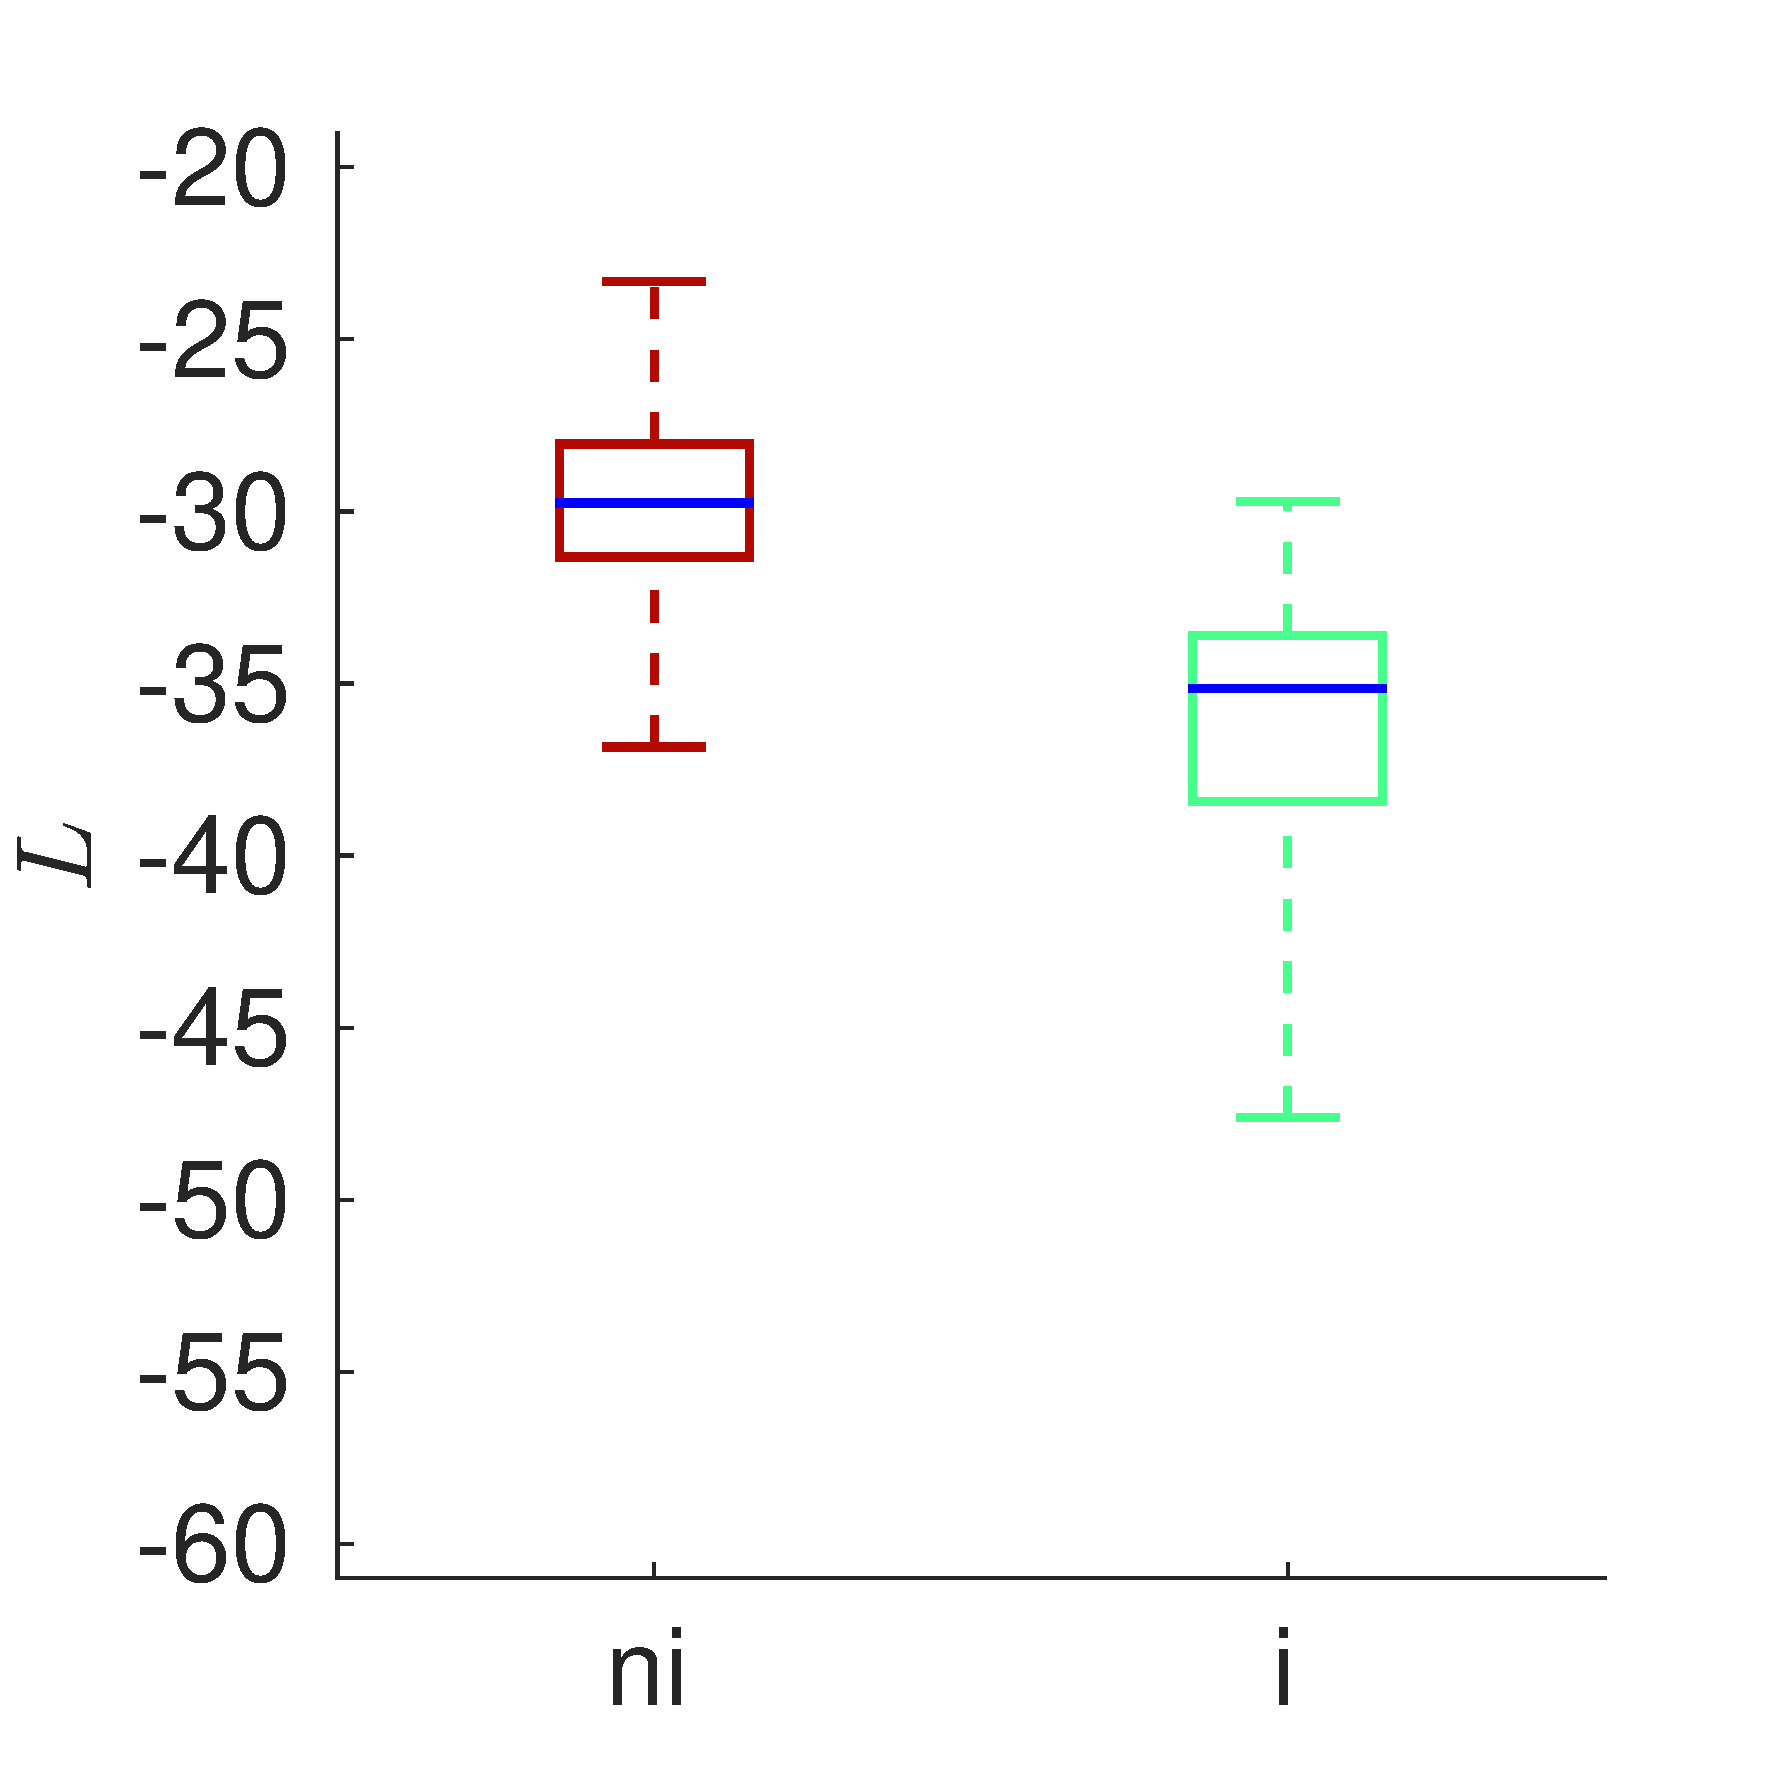
\includegraphics[width=.33\linewidth]{gfx/ch_5/xp_soundlevel_1}\label{fig:soundlevela}}
        \subfloat[]
        {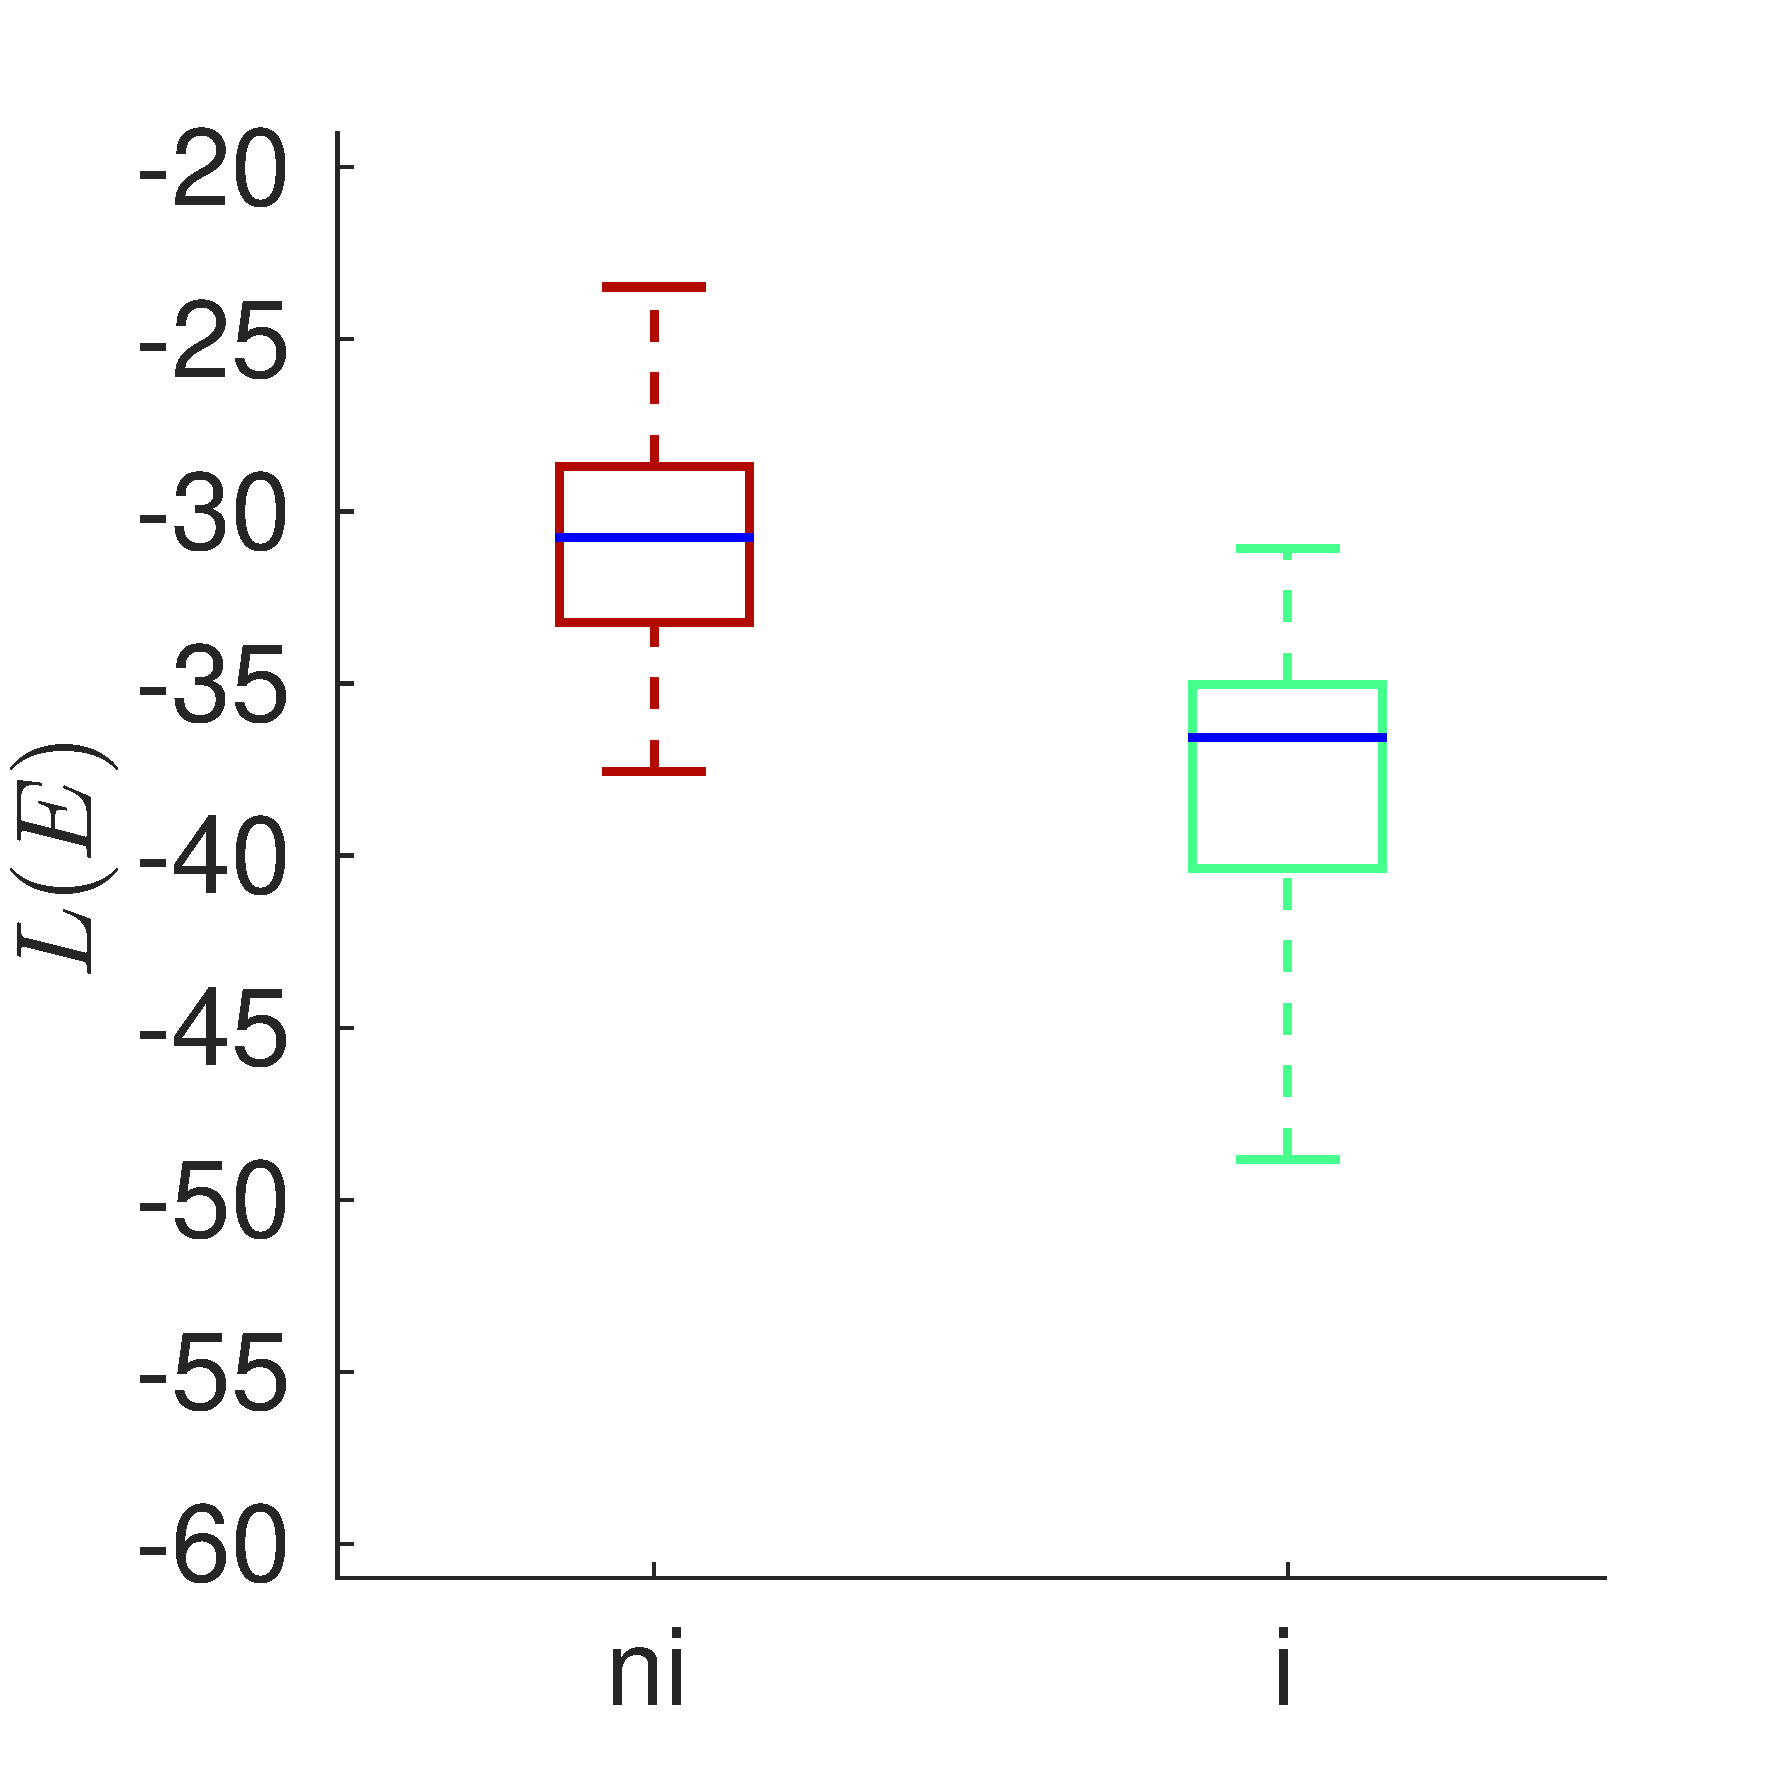
\includegraphics[width=.33\linewidth]{gfx/ch_5/xp_soundlevel_3}\label{fig:soundlevelb}}
        \subfloat[]
        {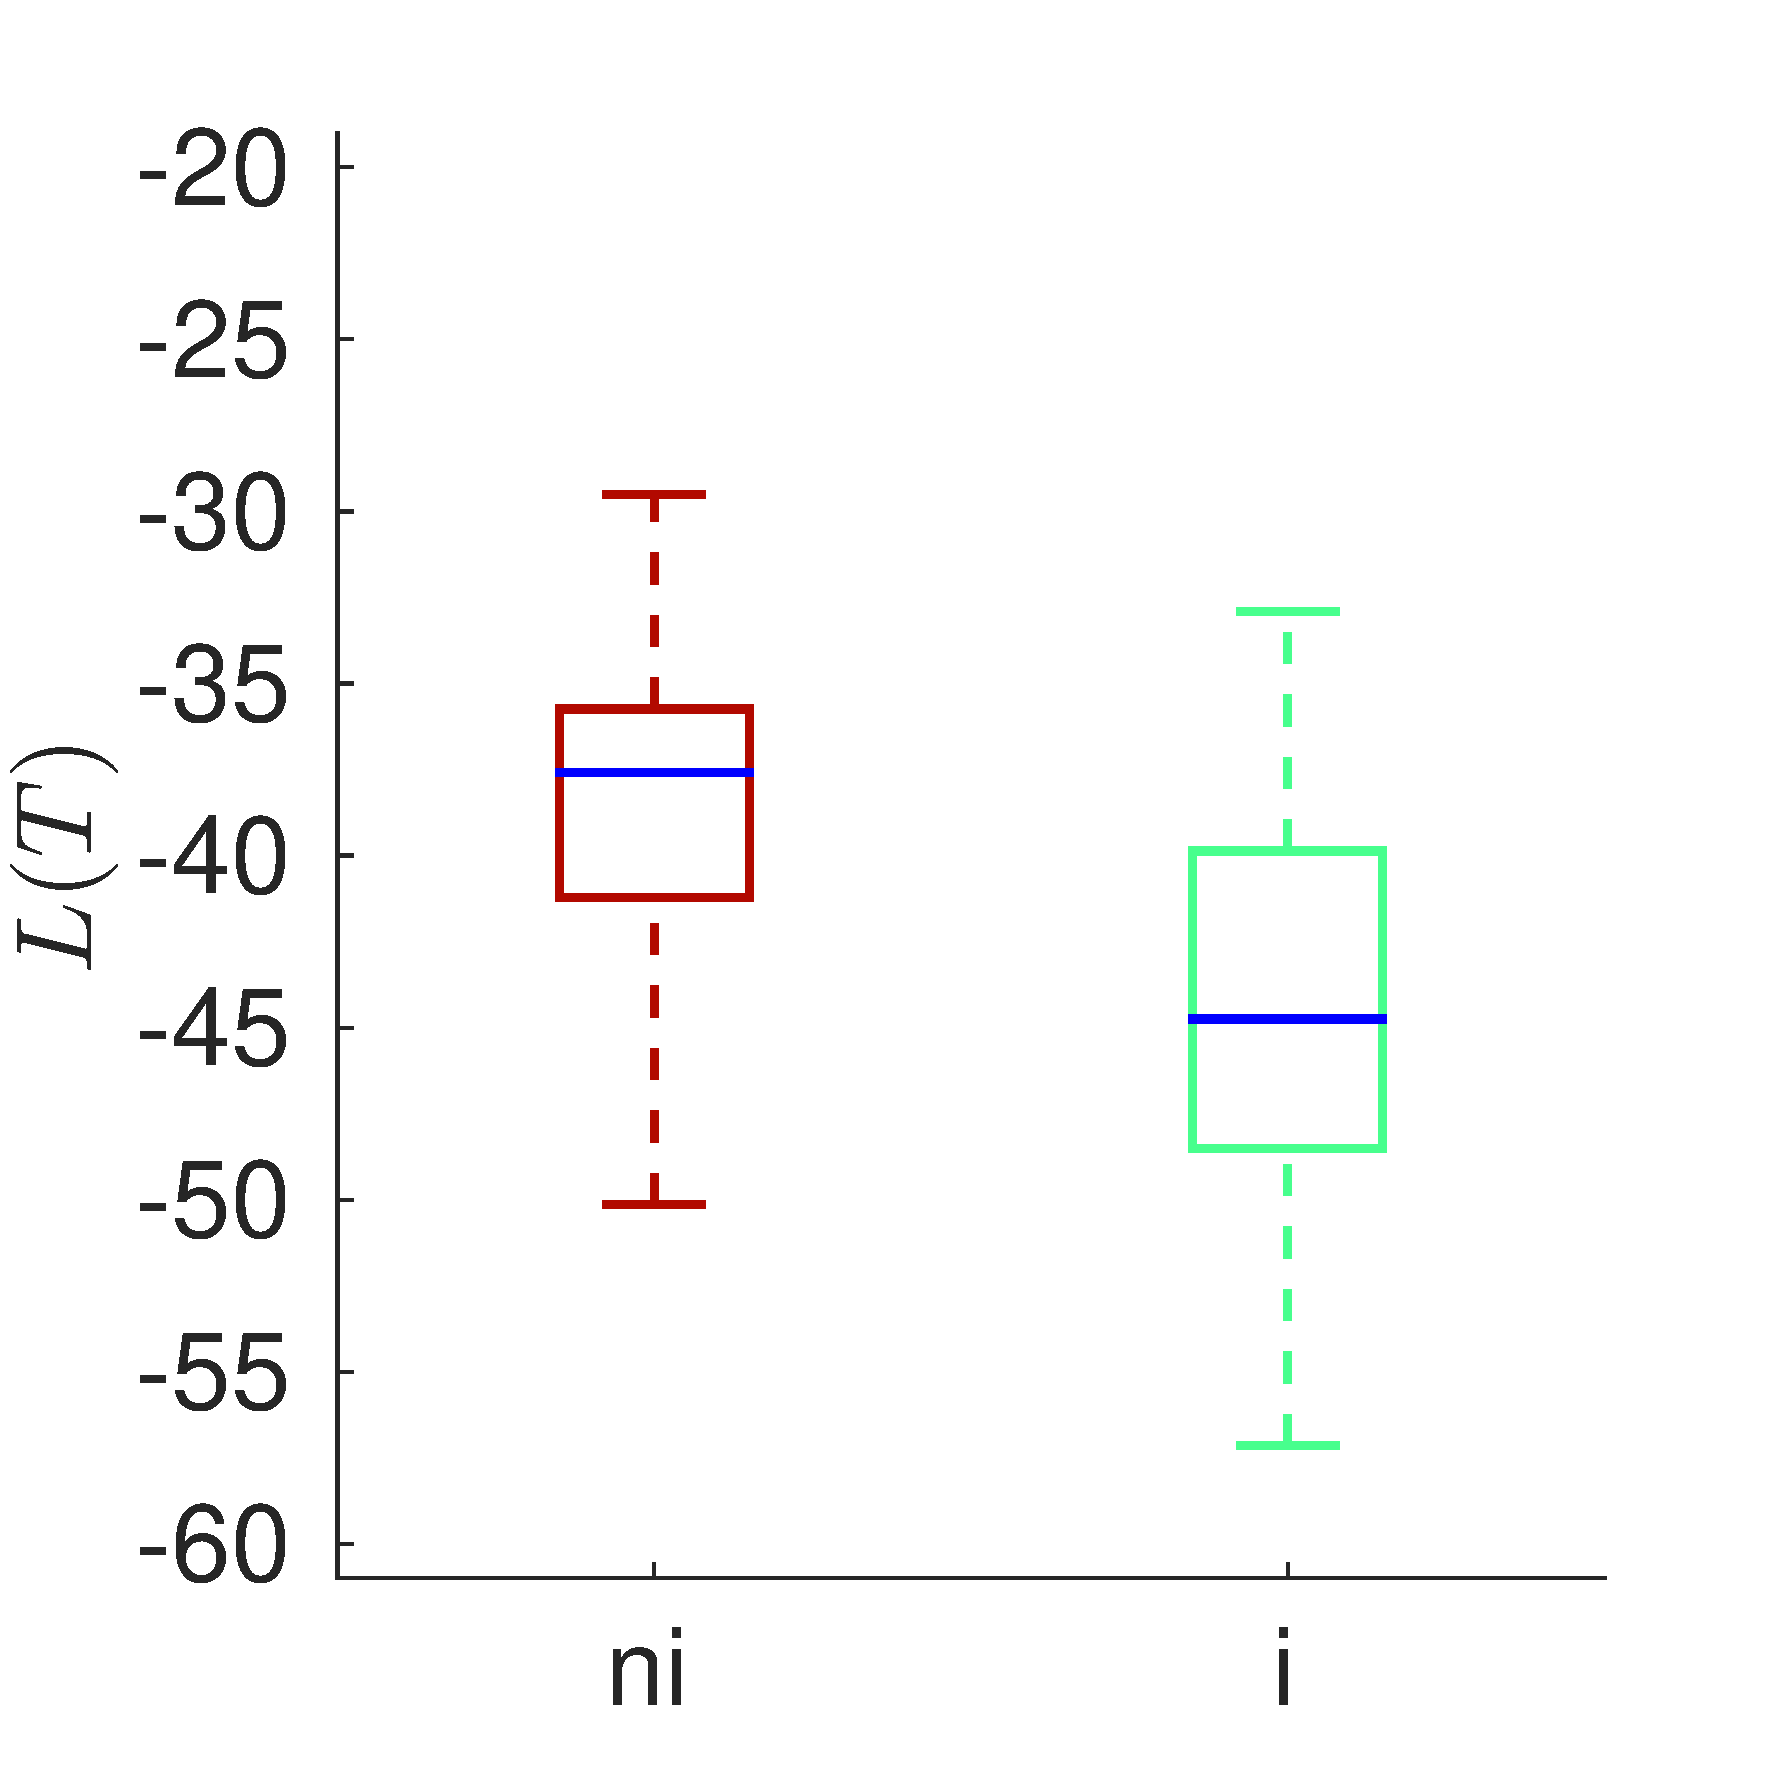
\includegraphics[width=.33\linewidth]{gfx/ch_5/xp_soundlevel_5}\label{fig:soundlevelc}}\par
        \subfloat[]
        {\includegraphics[width=.33\linewidth]{gfx/ch_5/xp_soundlevel_2}\label{fig:soundleveld}}
        \subfloat[]
        {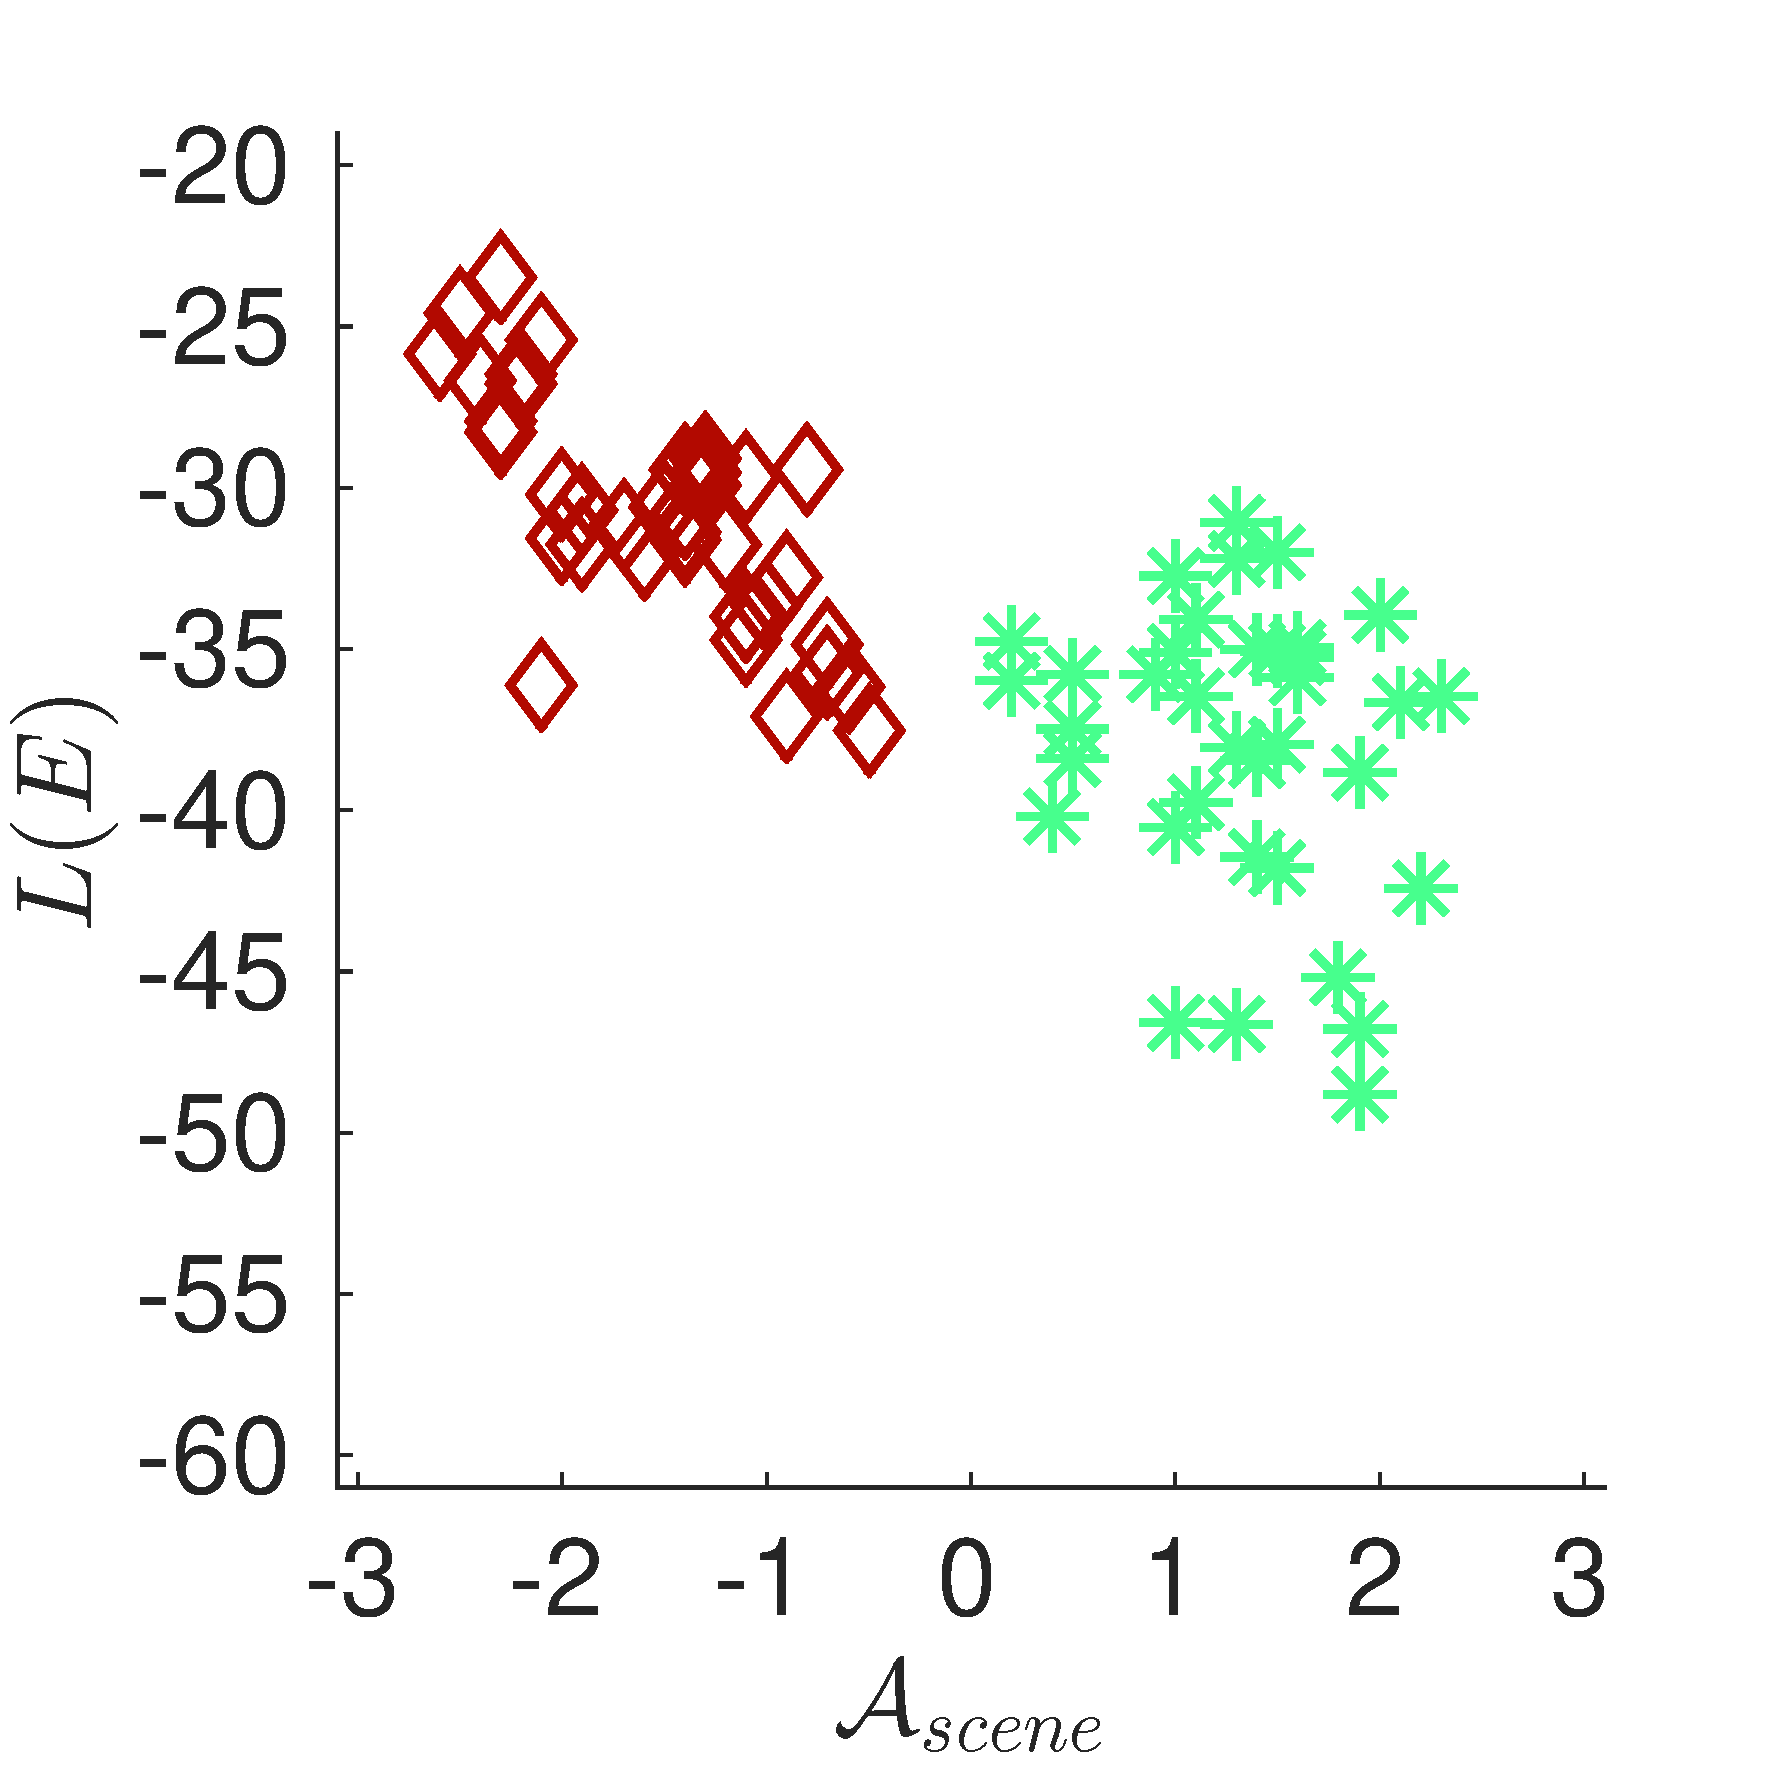
\includegraphics[width=.33\linewidth]{gfx/ch_5/xp_soundlevel_4}\label{fig:soundlevele}}
        \subfloat[]
        {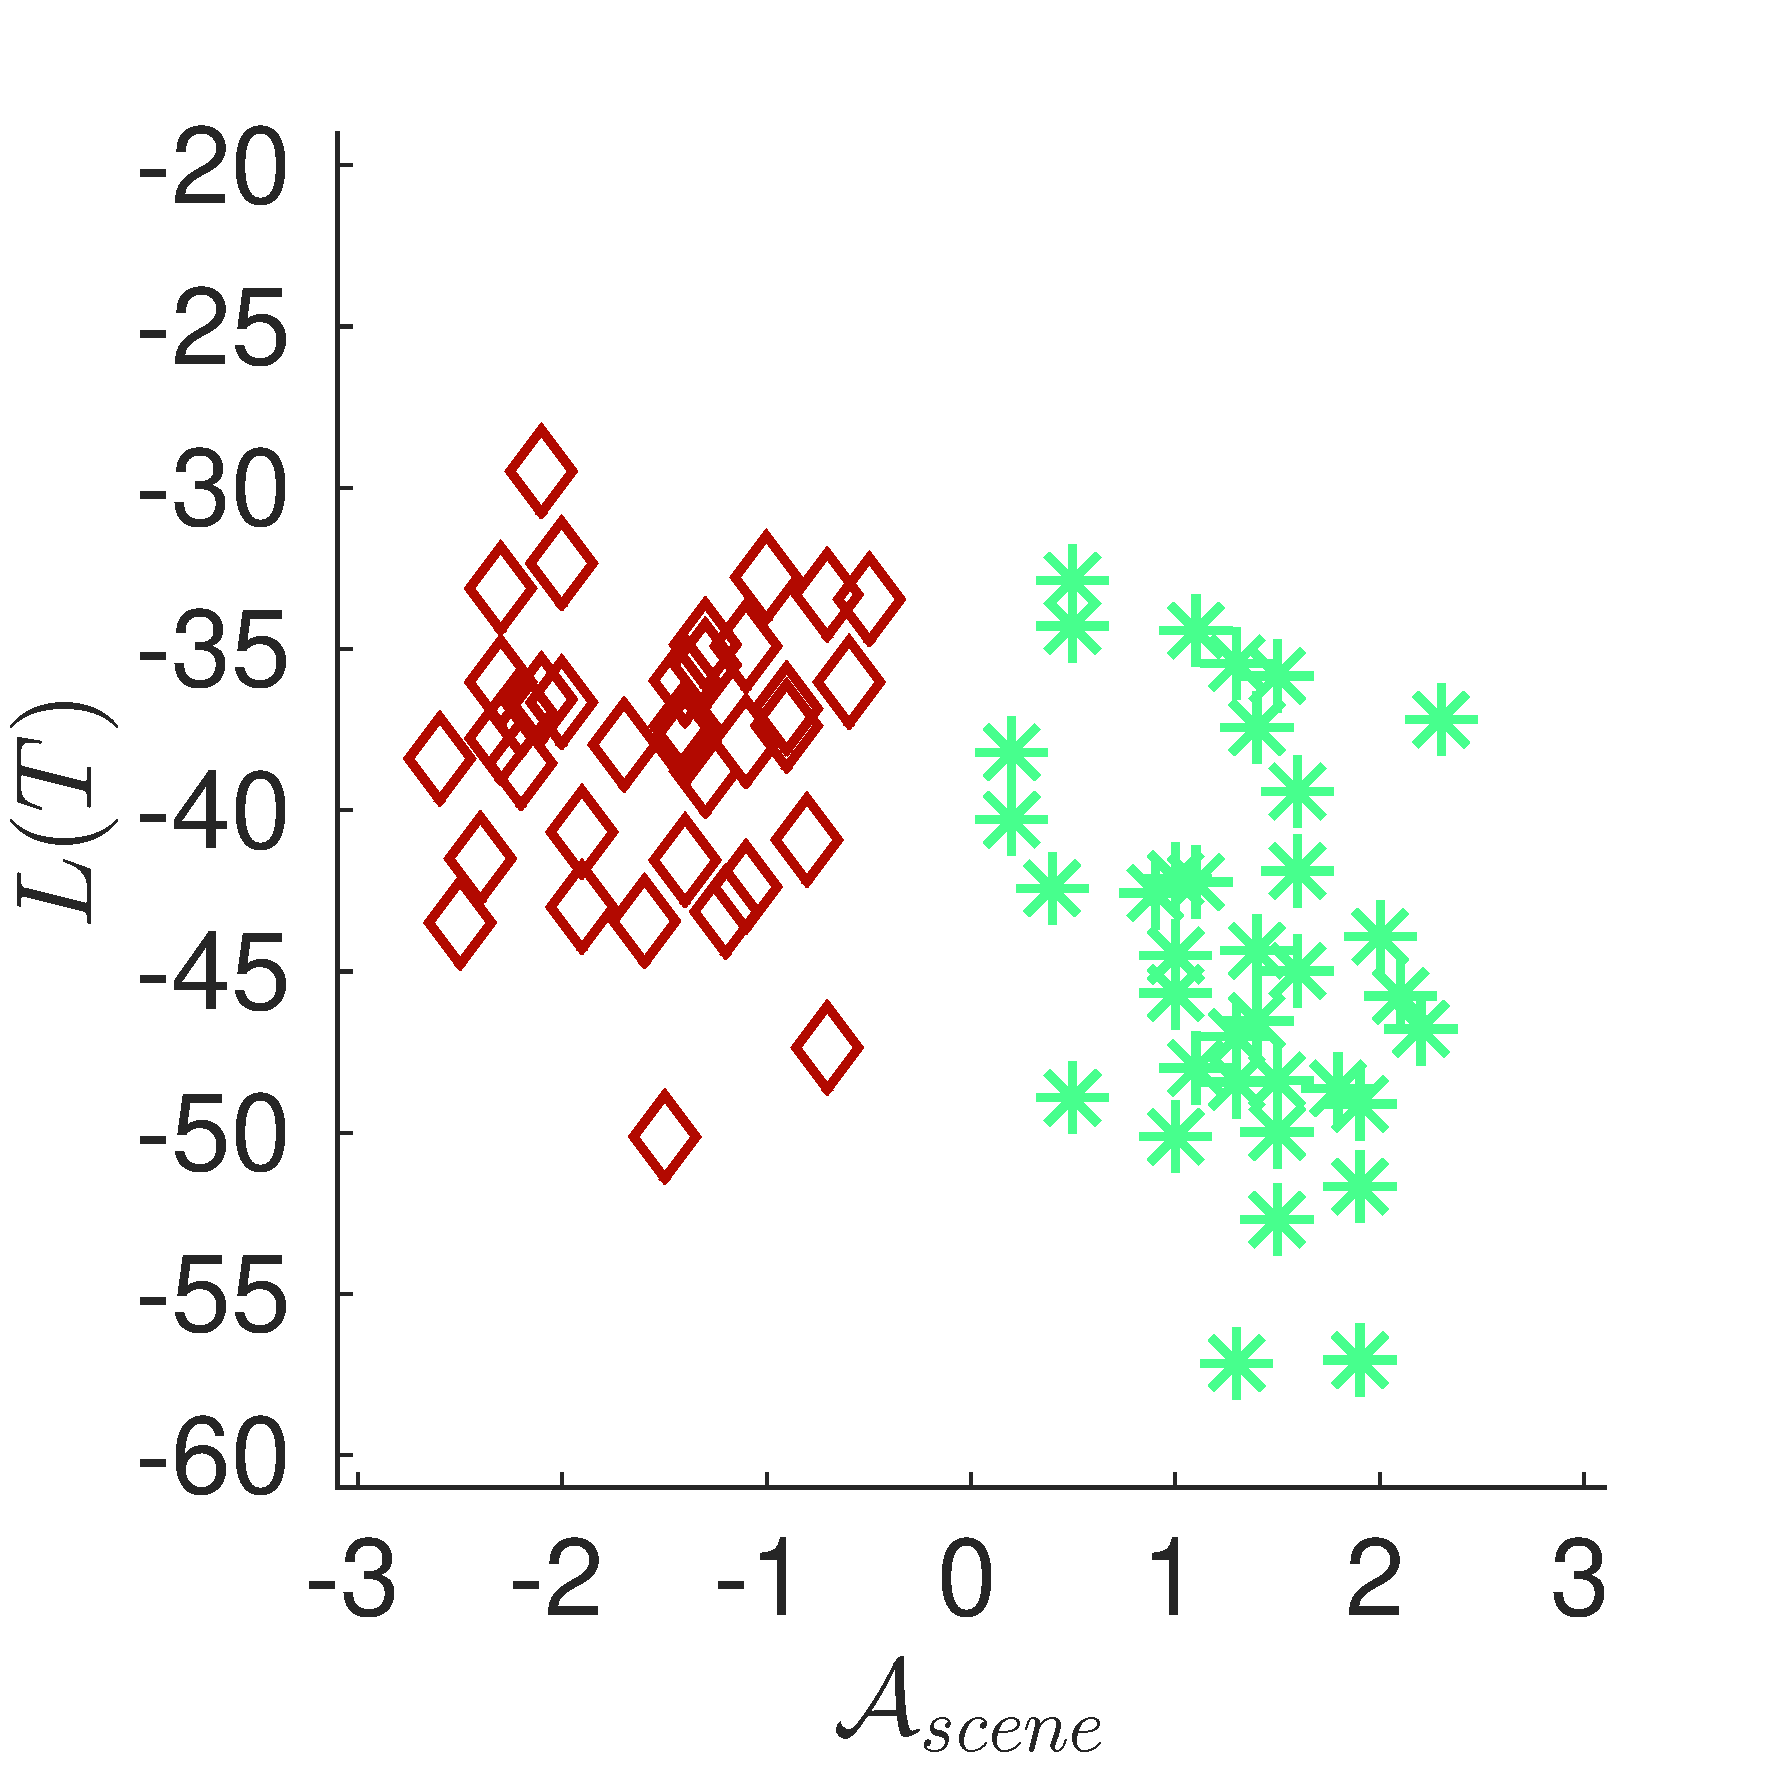
\includegraphics[width=.33\linewidth]{gfx/ch_5/xp_soundlevel_6}\label{fig:soundlevelf}}
       \caption{Dispersions des descripteurs structurels $L$ (a, d), $L(E)$ (b, e) et $L(T)$ (c, f), en fonction du type de scènes (a, b, c) et de l'agrément perçu $\mathcal{A}_{scene}$ de l'expérience 1.b (d, e, f).}
\end{figure}

\subsubsection*{Influence des descripteurs structurels sur l'agrément perçu}

Dans cette partie, nous analysons les relations fines qui peuvent exister entre les descripteurs structurels, d'une part, et l'agrément perçu, d'autre part. Contrairement à la section précédente, où la qualité affective des scènes est représentée de manière binaire (i \vs~ni), nous considérons ici l'agrément moyen $\mathcal{A}_{scene}$ comme descripteur perceptif. Il s'agit d'étudier l'existence de potentielles corrélations entre les descripteurs structurels et $\mathcal{A}_{scene}$. Les coefficients de corrélations linéaires calculés entre $\mathcal{A}_{scene}$ \vs~$L$, $L(E)$, $L(T)$ sont présentés dans le tableau~\ref{tab:corrStructA}. Les relations entre $\mathcal{A}_{scene}$ et les descripteurs structurels sont illustrées par les figures~\ref{fig:soundleveld},~\ref{fig:soundlevele} et ~\ref{fig:soundlevelf}.

Concernant $L$, on observe une forte corrélation négative ($r=-0.77$, $p<0.01$) avec $\mathcal{A}_{scene}$, indiquant que plus le niveau sonore est élevé, plus la scène est désagréable. Cependant, la figure~\ref{fig:soundleveld} suggère que cette relation ne s'opère pas de la même manière pour les i- et ni-scènes. En effet, la corrélation entre $L$ et $\mathcal{A}_{scene}$, pour les ni-scènes, reste élevée ($r=-0.78$, $p<0.01$), mais est inexistante pour les i-scènes.

Ce résultat, considérant l'ensemble des scènes, s'explique par le fait que les i-scènes ont tendance à être moins fortes que les ni-scènes, donnant ainsi l'illusion de prolonger la corrélation négative observée pour les ni-scènes.

Nous en concluons que $L$:

\begin{itemize}
\item permet bien de faire la distinction entre les i- et ni-scènes,
\item permet de finement caractériser l'agrément perçu des ni-scènes,
\item n'est pas un indicateur pertinent de l'agrément perçu pour des environnements a priori agréables.
\end{itemize}

Les mêmes constats sont faits concernant $L(E)$ (\cf~Figure~\ref{fig:soundlevele}). Pour $L(T)$ (\cf~Figure~\ref{fig:soundlevelf}), la corrélation modérée observée sur les scènes considérées dans leur globalité n'apparaît plus sur les i-scènes et ni-scènes considérées de façon séparée (i-scènes: $r=-0.33$, $p=0.05$, ni-scènes: $r=-0.00$, $p=0.99$). On peut penser que la corrélation négative émergeant au niveau l'ensemble est un artefact résultant du fait que le niveau des textures des i-scènes a tendance à être plus bas que celui des ni-scènes. Ainsi, si les événements sonores conservent une certaine capacité de prédiction de l'agrément pour les ni-scènes, le niveau des textures n'apporte, lui, que peu d'informations, quel que soit l'environnement.

En résumé, en présence d'un environnement désagréable, les niveaux sonores, en particulier ceux des événements, ont un impact négatif sur l'agrément. En présence d'un environnement agréable, en revanche, aucun des descripteurs structurels considérés ici ne semble influer sur la perception de l'agrément.

Ces premiers résultats pourraient montrer qu'il existe deux modes de perception, mobilisant chacun des descripteurs indépendants, modes qui s'activent en fonction de la nature de l'environnement (i ou ni).

Le fait que $L$ ne permet pas de caractériser l'agrément des i-scènes peut nous amener à penser que toutes les sources sonores ne contribuent pas de manière égale à la perception de l'agrément, mais que seules le niveau de certaines d'entre elles a une réelle influence. Afin d'approfondir ce point, nous analysons, dans la section suivante, les scènes d'un point de vue sémantique, \ie~en nous intéressant à la nature des sources qui les composent.


\begin{table}[t]
\centering
\begin{tabular}{l c c c}
               & i-scènes                   & ni-scènes    \\
\hline
$L$            & -0.32 ($p=0.06$)           & \textbf{-0.78} ($p<0.01$)\\
$L(E)$         & -0.20 ($p=0.24$)           & \textbf{-0.75} ($p<0.01$)\\
$L(T)$         & -0.33 ($p=0.05$)           &  -0.00 ($p=0.99$) \\
\hline
\end{tabular}
\vspace{0.5mm}
\caption{Coefficients de corrélation linéaire calculés entre l'agrément perçu moyen $\mathcal{A}_{scene}$ de l'expérience 1.b et les descripteurs structurels.}
\label{tab:corrStructA}
\end{table}

\subsubsection*{Analyse des descripteurs sémantiques}

Nous analysons la composition des scènes en comptant le nombre de sujets ayant utilisé une classe de sons pour simuler un type d'environnement. Les résultats sont présentés à la figure~\ref{fig:soundsourcea} pour les événements, et à la figure~\ref{fig:soundsourceb} pour les textures. Par souci d'espace, nous choisissons un niveau d'abstraction intermédiaire entre les niveaux 0 et 1, noté $0+$, pour représenter les classes (\cf~Figure~\ref{fig:taxonomie}).

Nous observons une différence notable dans le choix des classes entre les i- et ni-scènes. La répartition des classes est très proche de celle obtenue dans une étude similaire sur les environnements sonores urbains idéaux \cite{guastavino2006ideal}, \ie~les classes suggérant la présence humaine et la nature sont très présentes dans les i-scènes, a contrario, les classes désignant des sons mécaniques et/ou de travaux sont principalement utilisées pour les ni-scènes.

Ces résultats confirment un fait déjà observé: la nature sémantique des sources sonores joue un rôle prédominant dans l'appréciation de l'environnement \cite{raimbault2005urban,dubois2006cognitive}.

Nous notons quelques différences avec \cite{guastavino2006ideal}: les résultats obtenus par Guastavino montrent que les sons de \emph{transports publics} sont caractéristiques des environnements sonores urbains idéaux. Les auteurs attribuent cela au fait que la perception de l'agrément est, entre autre, soumise à un contexte socio-culturel. Dans notre représentation du monde, les sons de transports publics sont positivement connotés, et ont ainsi tendance à être mieux acceptés que les sons de véhicules privés.

Dans une certaine mesure, nos résultats contredisent ce fait. La figure~\ref{fig:soundsourcea} montre, en effet, que les classes d'événements de \emph{transports publics} (\emph{bus} et \emph{train}, \cf~Figure~\ref{fig:soundsourcec}) ont été utilisées par les sujets, pour des i-scènes, dans $28\%$ des cas, et pour des ni-scènes, dans $42\%$ des cas. Les résultats ne remettent pas en question le fait que les sons de \emph{transports publics} soient bien acceptés: $25\%$ des sujets ont utilisé la classe \emph{bus} pour les i-scènes, un chiffre comparable à celui de la classe \emph{Vélo}, et bien supérieur à celui de toute autre classe de véhicules privés. Cependant les classes \emph{transports publics} sont également bien présentes dans les ni-scènes, plus que les classes \emph{voiture} ou \emph{camion} par exemple. La classe \emph{transports publics} ne peut donc pas être considérée comme typique d'un environnement sonore urbain idéal.

Cette différence peut s'expliquer par la nature des deux protocoles expérimentaux utilisés. Comme nous l'avons fait, Guastavino demande à ses sujets de décrire un environnement. Mais ces derniers travaillent de mémoire, alors que nos propres sujets disposent de supports sonores. Le fait que nos sujets soient confrontés à la réalité acoustique des sons, pour recréer leurs environnements, peut avoir pour effet de diminuer l'impact du contexte socio-culturel. D'autres études utilisant des sons comme stimuli montrent que la classe \emph{bus} peut avoir un effet négatif sur l'appréciation de l'environnement \cite{lavandier2006contribution}.

\begin{figure}[t]
        \myfloatalign
        \subfloat[]
        {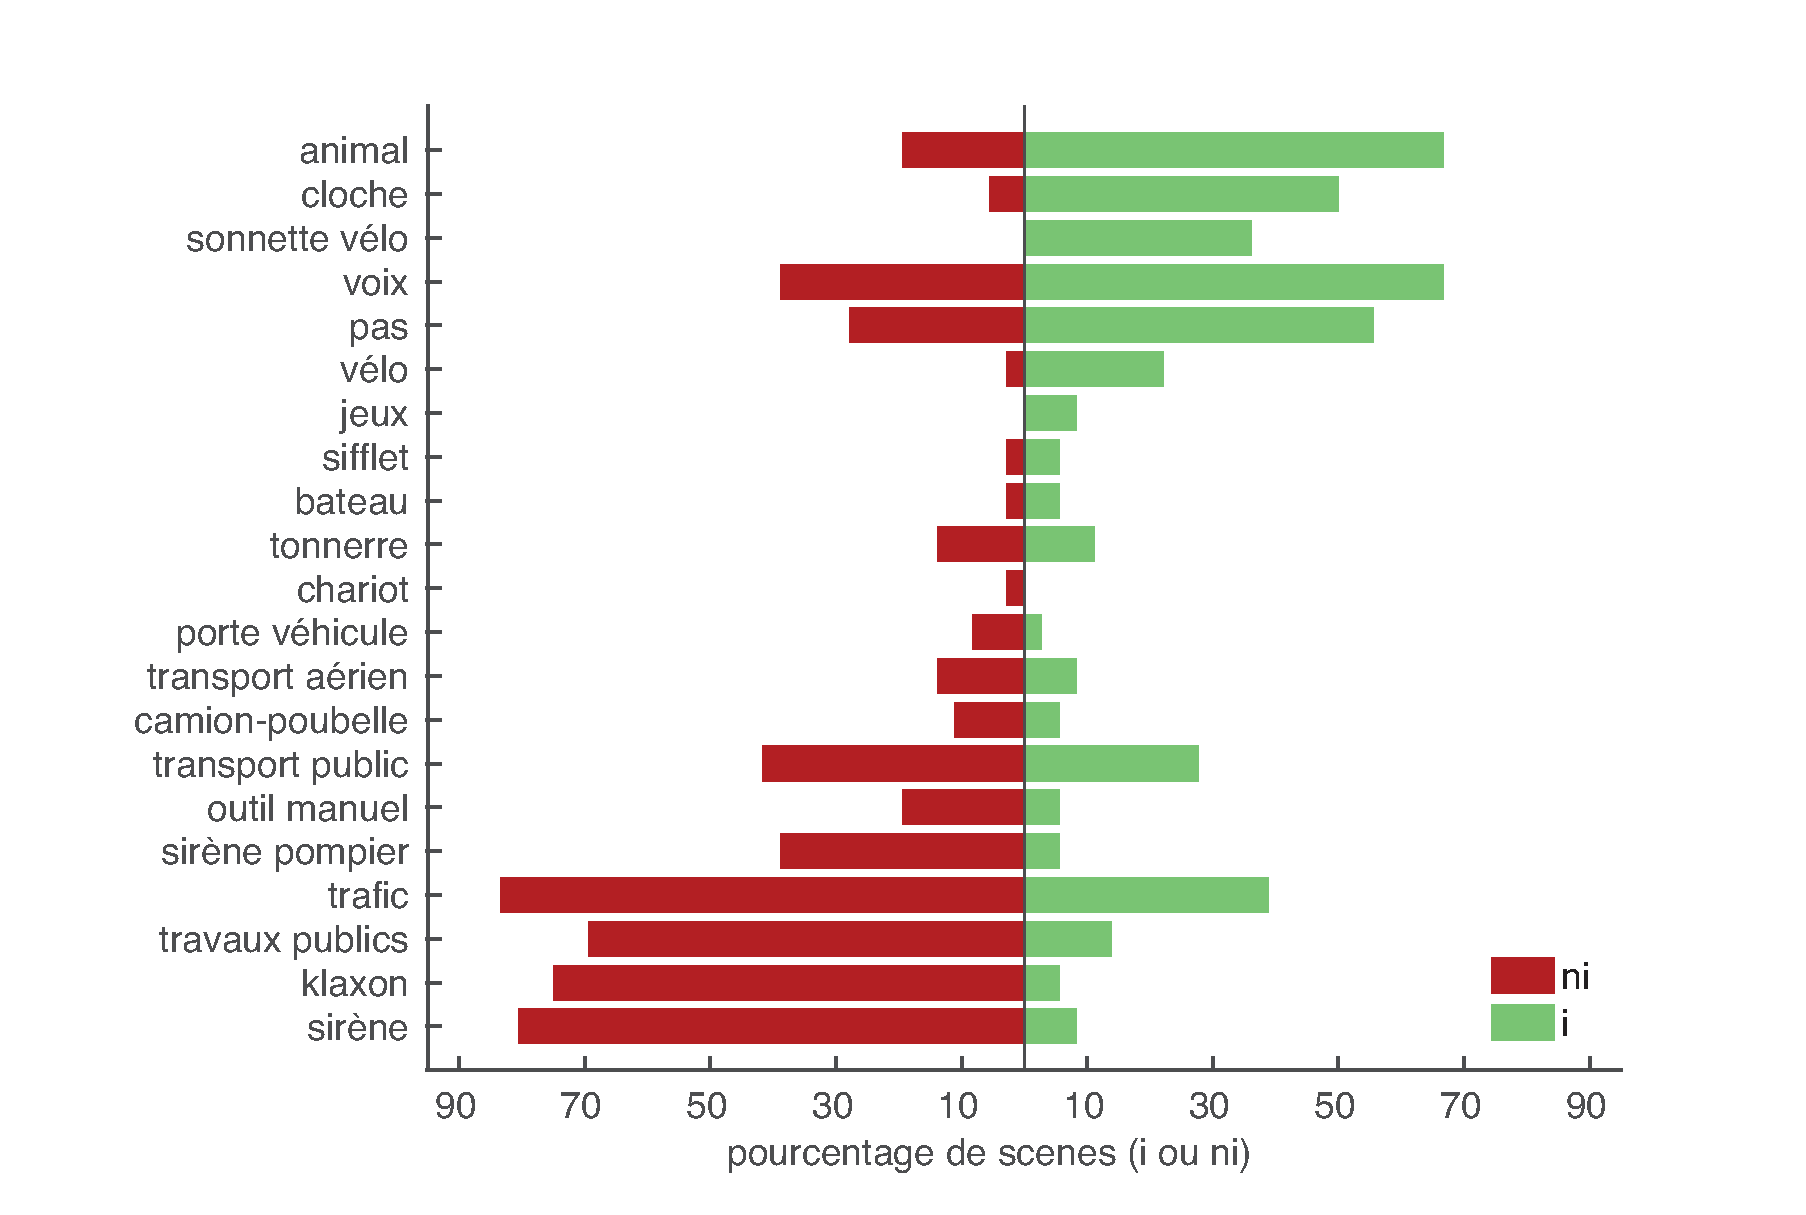
\includegraphics[width=1\linewidth]{gfx/ch_5/xp1_class_1_cam}\label{fig:soundsourcea}} \par
        \subfloat[]
        {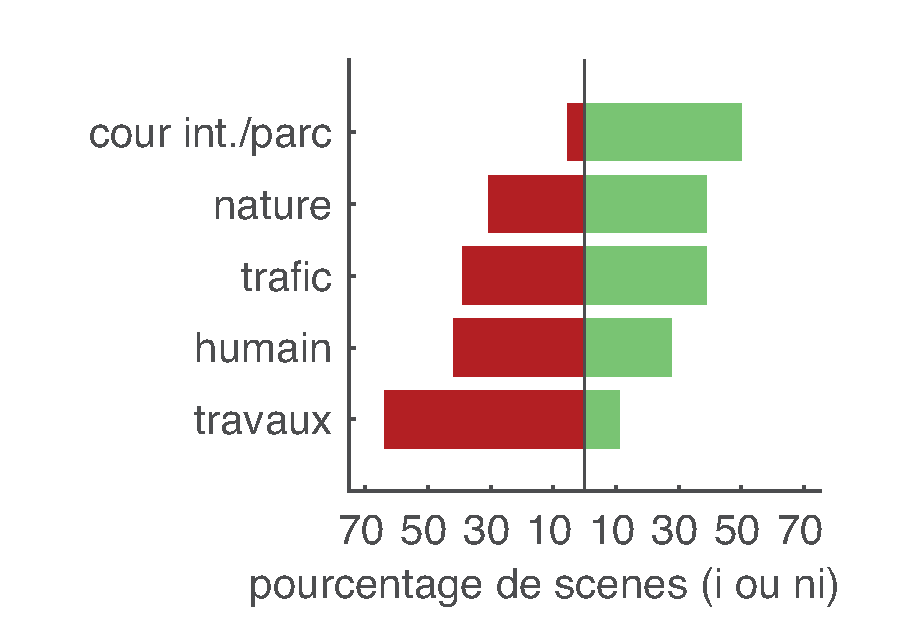
\includegraphics[width=.4\linewidth]{gfx/ch_5/xp1_class_2_cam}\label{fig:soundsourceb}}
        \subfloat[]
        {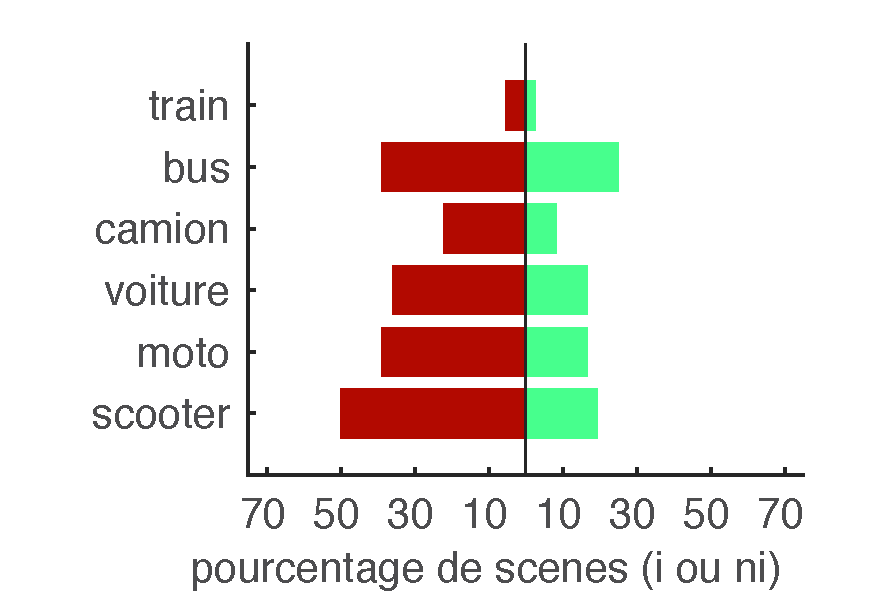
\includegraphics[width=.4\linewidth]{gfx/ch_5/xp1_class_3_cam}\label{fig:soundsourcec}}
       \caption{Pourcentage de scènes simulées (i ou ni) comportant une classe de son particulière: (a) classes d'événements du niveau d'abstraction $0+$, (b) classes de textures du niveau d'abstraction $0$, (c) sous classes d'événements du niveau d'abstraction $1$ appartenant aux classes \emph{trafic} et \emph{transport public} du niveau d'abstraction $0$.}\label{fig:soundsource}
\end{figure}

\subsubsection*{Marqueurs sonores}

Nous avons mis en évidence que, qualitativement, la composition des sources sonores des scènes diffère selon les types d'environnement (i ou ni). Nous essayons de voir maintenant si, parmi ces classes, certaines sont typiques d'un environnement en particulier. Pour ce faire, nous utilisons le V-test (\cf~Section~\ref{sec:xp1_dataAna}), en considérant séparément chaque niveau d'abstraction. Les résultats sont présentés dans le tableau~\ref{tab:markers}.

Concernant les événements sonores, 9 marqueurs sont identifiés sur l'ensemble des niveaux d'abstraction. Comme la figure~\ref{fig:soundsource} le laissait présager, les classes relatives à la présence humaine (\emph{pas homme béton}, \emph{sonnette vélo}), et à la nature (\emph{animaux, oiseaux}, \emph{chants d'oiseaux}) sont des marqueurs de i-scènes. Nous notons également la présence de la classe \emph{cloche} dans les marqueurs d'un environnement idéal. Ce fait est possiblement dû au \emph{background} socio-culturel des sujets, dans leur grande majorité, des citoyens européens. En effet, selon Schafer, un son reconnu par un individu comme faisant partie intégrante de son environnement est bien accepté. Les marqueurs de ni-scènes sont des classes faisant référence à des sons de travaux (\emph{travaux}), ou suggérant un trafic dense (\emph{klaxon}, \emph{sirène}).

Concernant les textures sonores, 5 marqueurs sont identifiés. Pour les i-scènes, il s'agit de classes faisant référence à des ambiances amorphes, calmes, (\emph{cour-intérieur} et \emph{parc}). Pour les ni-scènes, il s'agit, comme pour les événements, de classes faisant référence à des bruits de travaux (\emph{travaux} et \emph{véhicule de travaux}), ainsi que d'une classe faisant référence au trafic (\emph{carrefour}).

Bien que l'ensemble des marqueurs identifiés soient intuitifs, aucune des classes d'événements faisant directement référence aux bruits de véhicules motorisés n'est un marqueur, exception faite de la classe de textures \emph{carrefour}. Pour représenter un trafic désagréable, les sujets ont porté leurs choix sur les classes \emph{klaxon} et \emph{sirène}. On peut supposer que les sons isolés de véhicules sont compris comme faisant partie intégrante de l'environnement urbain, et ne sont donc pas particulièrement associés à un environnement désagréable.

\begin{table}[t]
 \setlength{\tabcolsep}{0.2pt}
 \centering
  {\renewcommand{\arraystretch}{0.9}
\begin{tabular}{c c c c}
Niveau        & \multicolumn{2}{c}{Marqueurs sonores événements} \\
d'abstraction & i-scènes & ni-scènes \\
\hline
0  &                          & travaux (3.78)  \\
\hline
  & cloche  (4.5)             & klaxon  (3.9) \\
1 & sonnette vélo  (4.3)      & sirène (3.9)\\
  & animal (4.2)              &       \\
   \hline
  & oiseau        (4.8)       & klaxon  (4.0)\\
2 & cloche  (4.4)             & sirène (4.0)\\
  & sonnette vélo    (4.2)             &       \\
   \hline
  & chant oiseau (4.8)        & klaxon  (4.1)\\
3 & cloche   (4.3)            & sirène (4.0)\\
  & sonnette vélo     (4.2)   &       \\
  & pas chaussure  (3.6)      &  \\
  &                           & \\
  & \multicolumn{2}{c}{Marqueurs sonores textures}      \\
  & i-scènes & ni-scènes \\
\hline
0 &     cour int./parc (4.1) &  travaux (3.9)  \\
\hline
1 &     parc (3.65)          &  carrefour (3.6)  \\
  &                          &  travaux véhicule (3.3)  \\
\hline
2 &     parc (3.64)          &  carrefour (3.56)  \\
\hline
\end{tabular}
}
\vspace{0.5mm}
\caption{Classes d'événements et de textures identifiées comme étant des marqueurs sonores. Dans chaque cellule, les marqueurs sont ordonnés par ordre décroissant de valeur $V$.}
\label{tab:markers}
\end{table}

\subsubsection*{Espaces de représentation induits par les descripteurs sémantiques}

Dans cette partie, nous évaluons la capacité d'une représentation sémantique à séparer les deux types d'environnement. Pour ce faire, nous calculons une précision au rang 5 ($p@5$) sur l'espace induit par les descripteurs sémantiques $S$, et ce pour chaque niveau d'abstraction (\cf~Section~\ref{sec:xp1_dataAna}). Les vecteurs $S$ sont construits en utilisant toutes les classes ($ET$), les classes d'événements ($E$), les classes de textures ($T$), les classes d'événements ne considérant que les marqueurs sonores ($E_m$), les classes d'événements ne considérant pas les marqueurs sonores $E_{w/o,m}$. Nous ne considérons pas les classes de marqueurs de textures, ces dernières étant trop peu nombreuses. Pour les mêmes raisons nous ne considérons pas les classes de marqueurs d'événements du niveau d'abstraction $0$. Les résultats sont affichés sur la figure~\ref{fig:pa5}.

En ce qui concerne $ET$, la $p@5$ est de $76\%$ pour le niveau d'abstraction 0, et reste supérieure à $86\%$ à partir du niveau d'abstraction 1. Ces résultats confirment qu'il est possible de clairement distinguer les deux types d'environnement en se basant seulement sur la présence ou l'absence des classes de sons. Nous notons également que, plus le niveau d'abstraction est élevé, plus la capacité de séparer les environnements est importante. En d'autres termes, plus nous sommes précis dans notre description de la composition des scènes, plus nous sommes à même d'établir une distinction claire entre les i- et ni-scènes.

En considérant séparément $E$ et $T$, il apparaît 1) que la $p@5$ obtenue avec $E$ est similaire à celle obtenue avec $ET$, 2) que la $p@5$ obtenue avec $T$ est systématiquement inférieure d'environ $10$ à $15\%$ à celle de $E$. Ces résultats indiquent que l'information sémantique permettant de séparer les deux environnements est principalement portée par les événements. Ces résultats font, par ailleurs, écho aux travaux de  \cite{maffiolo_caracterisation_1999}, qui montrent que nous analysons de manière descriptive (en identifiant les sources) les scènes événementielles, \ie~composées d'événements sonores (\cf~Section~\ref{sec:simscene_sampleDataSet}).

Enfin, il apparaît que la $p@5$ obtenue avec $E_{m}$ est égale, voire supérieure à celles obtenues avec $E$ et $ET$, et ce bien qu'une information partielle soit utilisée dans ce cas pour décrire les scènes. La dimension des vecteurs de description $S$ pour $E_m$ est en effet inférieure à la dimension des vecteurs $S$ pour $E$, qui est elle même inférieure à celle obtenue dans le cas où toutes les classes sont utilisées ($ET$). De plus, dans le cas où les marqueurs ne sont pas pris en compte pour la description ($E_{w/o,m}$), les résultats chutent, passant même en dessous de ceux obtenus en ne considérant que les textures. Cela confirme que la majorité de l'information sémantique permettant de faire la distinction entre i-scènes et ni-scènes est incluse dans les marqueurs.

En résumé, nous déduisons de cette analyse les points suivants:

\begin{enumerate}
\item contrairement à ce que nous avions constaté avec les descripteurs structurels, une description sémantique de la composition des scènes, en terme de présence/absence de sources sonores, permet de bien distinguer les deux types d'environnement (i ou ni);
\item l'information sémantique est majoritairement portée par les classes d'événements sonores;
\item parmi les classes d'événements, seule une partie, \ie~les marqueurs sonores, est nécessaire pour faire la distinction entre les i- et ni-scènes.
\end{enumerate}

Maintenant que nous avons isolé les classes typiques des i- et ni-scènes, et vérifié que la distinction entre ces environnements dépendait de la présence de ces classes, il reste à voir si une description structurelle des scènes, basée uniquement sur ces marqueurs sonores, permet de caractériser l'agrément perçu, mieux qu'une description structurelle globale.

\begin{figure}[t]
        \myfloatalign
        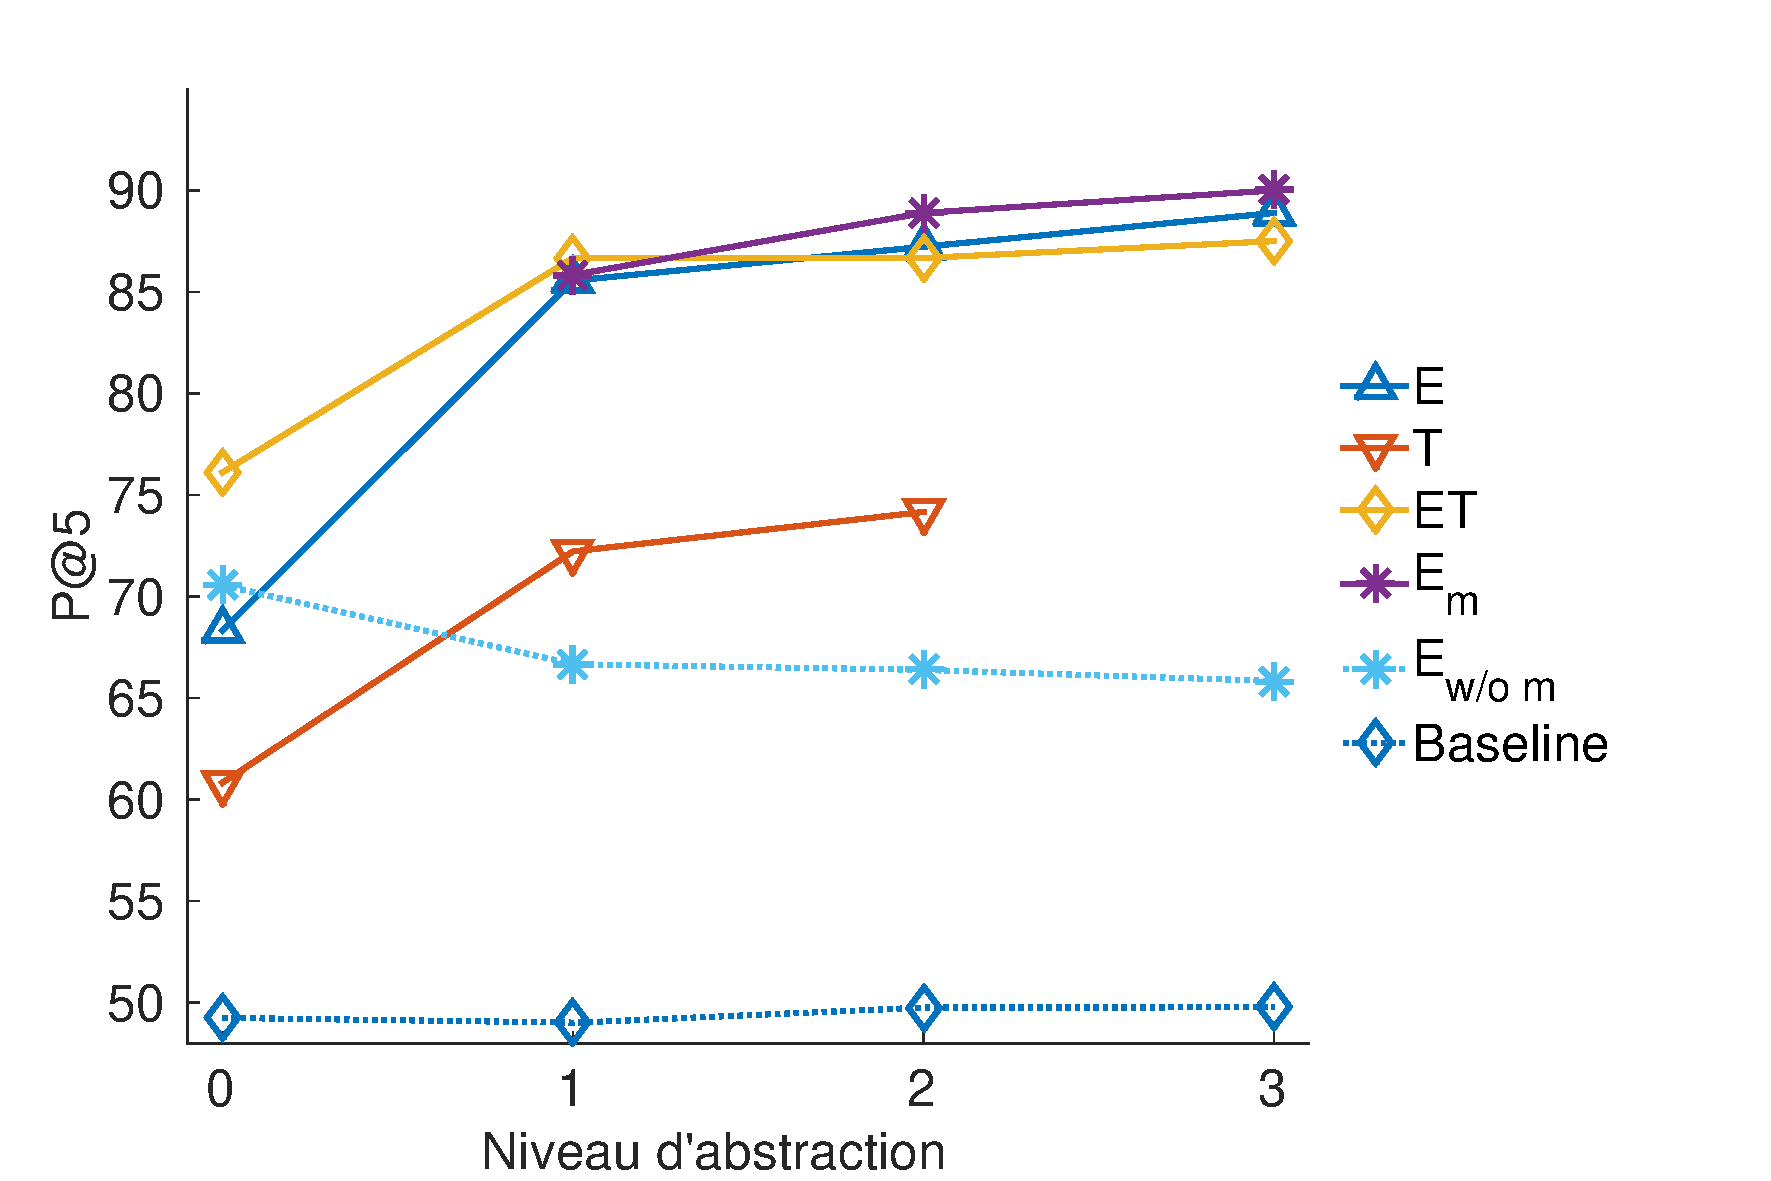
\includegraphics[width=\linewidth]{gfx/ch_5/pa5_1}
       \caption{$P@5$ obtenues en considérant la matrice de dissimilarité résultant des distances par paires de Hamming calculées entre les vecteurs des descripteurs sémantiques des scènes. Les vecteurs sont construits en utilisant toutes les classes ($ET$), les classes d'événements ($E$), les classes de textures ($T$), les classes d'événements ne considérant que les marqueurs sonores ($E_m$), les classes d'événements ne considérant pas les marqueurs sonores $E_{w/o,m}$.}\label{fig:pa5}
\end{figure}

\subsubsection*{Influence des marqueurs sonores sur l'agrément perçu}

Nous évaluons les corrélations entre $\mathcal{A}_{scene}$ et les descripteurs structurels. Pour cette section, les descripteurs structurels sont calculés en tenant compte des marqueurs sonores précédemment identifiés. Nous définissons $X_m$ le descripteur $X$ calculé en ne prenant en compte que les sons des marqueurs. A l'inverse, nous définissons $X_b$ ($b$: pour «~bruit~») le descripteur $X$ calculé en prenant en compte toutes les classes de sons, excepté les marqueurs. Lorsque le descripteur caractérise une i-scène (idem pour une ni-scène), nous ne considérons, pour le calcul, que les marqueurs identifiés pour les i-scènes (ou pour les ni-scènes), que nous nommons i-marqueurs (ou ni-marqueurs). Les résultats sont affichés sur le tableau~\ref{tab:corrMarkers}.

Concernant les niveaux sonores (\cf~Figures~\ref{fig:soundlevelMarkera} et~\ref{fig:soundlevelMarkerd}), les mêmes tendances sont observées entre $L_m$, $L(E)_m$ et $L(T)_m$, d'une part, et $L$, $L(E)$ et $L(T)$, d'autre part. Que l'on considère uniquement les marqueurs, ou l'ensemble des classes, il s'avère que :

\begin{enumerate}
\item il existe une différence significative entre les niveaux des i- et ni-scènes ($L_m$, $L(E)_m$ et $L(T)_m$: $p<0.01$);
\item le niveau sonore des scènes est majoritairement porté par les événements sonores, comparé aux textures sonores;
\item le niveau sonore des événements a une influence sur la perception de l'agrément pour les ni-scènes, mais pas pour les i-scènes;
\item le niveau sonore des textures ne joue aucun rôle dans la perception de l'agrément.
\end{enumerate}

En conclusion, le niveau des ni-marqueurs a une influence négative sur l'agrément pour les ni-scènes. En revanche le niveau des i-marqueurs n’impacte pas l'agrément perçu pour les i-scènes.

En considérant maintenant les classes non marqueurs (\cf~Figures~\ref{fig:soundlevelNoisea} et~\ref{fig:soundlevelNoised}), nous remarquons, sur les i-scènes, une corrélation négative modérée/faible pour $L_b$  ($r=-52$, $p<0.01$) et $L(E)_b$ ($r=-51$, $p<0.01$). C'est la première fois qu'un indicateur objectif nous permet de préciser l'agrément des environnements agréables. Ceci nous amène à conclure que le niveau des classes de sons n'étant pas typiques d'un environnement agréable a un impact négatif sur l'agrément.

Par ailleurs, alors que $L(T)$ ne présentait pas de corrélation pour les ni-scènes, une corrélation négative forte est observée pour $L(T)_b$ ($r-0.73$, $p<0.01$). Ce fait indique que les niveaux des classes de textures n'étant pas des marqueurs n'affectent pas l'agrément perçu de la même manière pour les i- et ni-scènes. Les niveaux semblent avoir un effet négatif pour les ni-scènes, alors que pour les i-scènes, aucun effet n'est relevé.

Pour finir, nous considérons un dernier groupe de descripteurs, nommément $L_m-L_b$, $L(E)_m-L(E)_b$ et $L(T)_m-L(T)_b$ (\cf~Figures~\ref{fig:soundlevelMarkerDiffa} et~\ref{fig:soundlevelMarkerDiffd}). Ces descripteurs expriment la différence entre les niveaux des marqueurs, et ceux des autres classes de sons. Ils traduisent l'émergence des marqueurs par rapport à la mixture sonore.

Pour les i-scènes, une corrélation modérée et positive est observée pour $L_m-L_b$ ($r=0.67$, $p<0.01$) et $L(E)_m-L(E)_b$ ($r=0.66$, $p<0.01$). Pour les ni-scènes, aucune corrélation n'est observée. Dans le cas des i-scènes, ce n'est donc pas le niveau absolu des marqueurs qui importe, mais leur niveau relatif, par rapport aux autres sons qui composent la scène. On observe donc pour les environnements idéaux un double mécanisme perceptif:

\begin{itemize}
\item plus le niveau absolu des sons n'étant pas des i-marqueurs est élevé, plus l'agrément est faible,
\item plus le niveau relatif des i-marqueurs, par rapport aux autres sons, est élevé, plus l'agrément est élevé.
\end{itemize}

Pour les ni-scènes, le fait que nous observions des corrélations pour $L_m$ et $L(E)_m$, et aucune pour $L_m-L_b$ et $L(E)_m-L(E)_b$, montre que c'est bien le niveau absolu qui importe.

\begin{table}[t]
\setlength{\tabcolsep}{3pt}
\centering
{\renewcommand{\arraystretch}{1}
\centering
\begin{tabular}{l r r}
                  &   i-scenes                  & ni-scenes \\
\hline
$L_m$              & 0.03  ($p=0.88$)           & \textbf{-0.75} ($p<0.01$) \\
$L(E)_m$           & 0.08  ($p=0.66$)           & \textbf{-0.71} ($p<0.01$) \\
$L(T)_m$           & -0.11 ($p=0.66$)           & -0.17 ($p=0.37$) \\
$L_b$              & \textbf{-0.52} ($p<0.01$)  & -0.32 ($p=0.06$) \\
$L(E)_b$           & \textbf{-0.51} ($p<0.01$)  & -0.30 ($p=0.07$) \\
$L(T)_b$           & -0.32 ($p=0.05$)           & \textbf{-0.73} ($p<0.01$) \\
$L_m-L_b$          & \textbf{0.67} ($p<0.01$)   & -0.31 ($p=0.07$) \\
$L(E)_m-L(E)_b$    & \textbf{0.66} ($p<0.01$)   & -0.28 ($p=0.10$) \\
$L(T)_m-L(T)_b$    & 0.16 ($p=0.54$)            & 0.21 ($p=0.28$) \\
\hline
\end{tabular}
}
\vspace{0.5mm}
\caption{Coefficients de corrélation linéaire calculés entre l'agrément perçu moyen $\mathcal{A}_{scene}$ de l'expérience 1.b et les descripteurs structurels relatifs à la présence des marqueurs sonores.}
\label{tab:corrMarkers}
\end{table}

\begin{figure}[t]
        \myfloatalign
        \subfloat[]
        {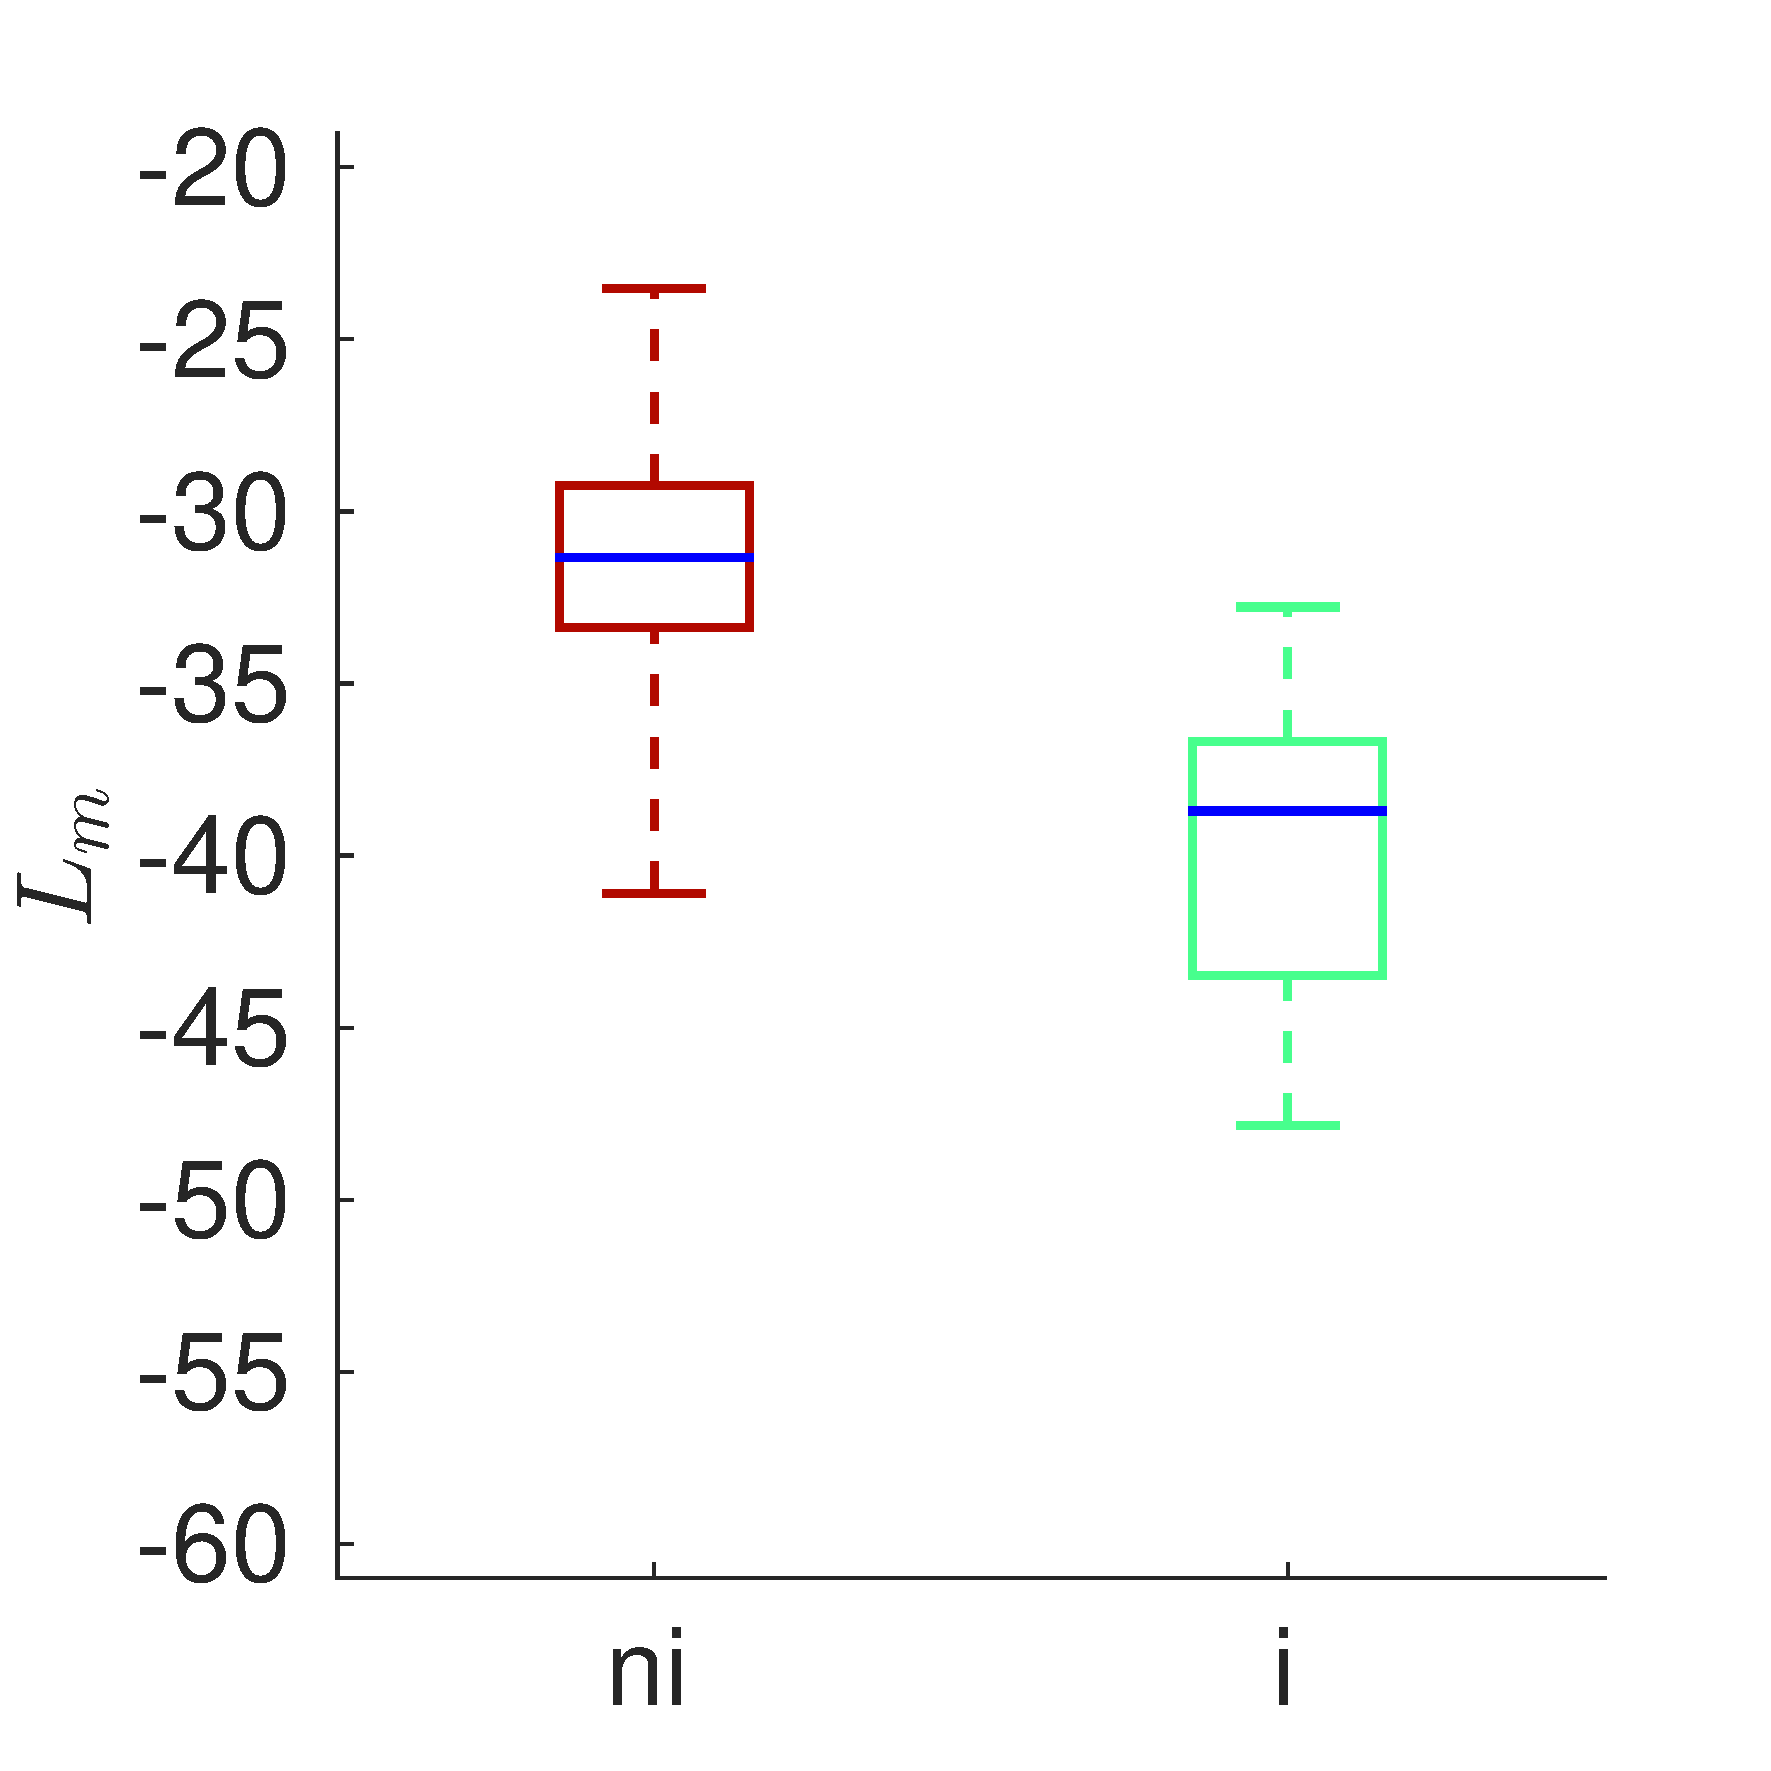
\includegraphics[width=.33\linewidth]{gfx/ch_5/xp_soundlevel_7}\label{fig:soundlevelMarkera}}
        \subfloat[]
        {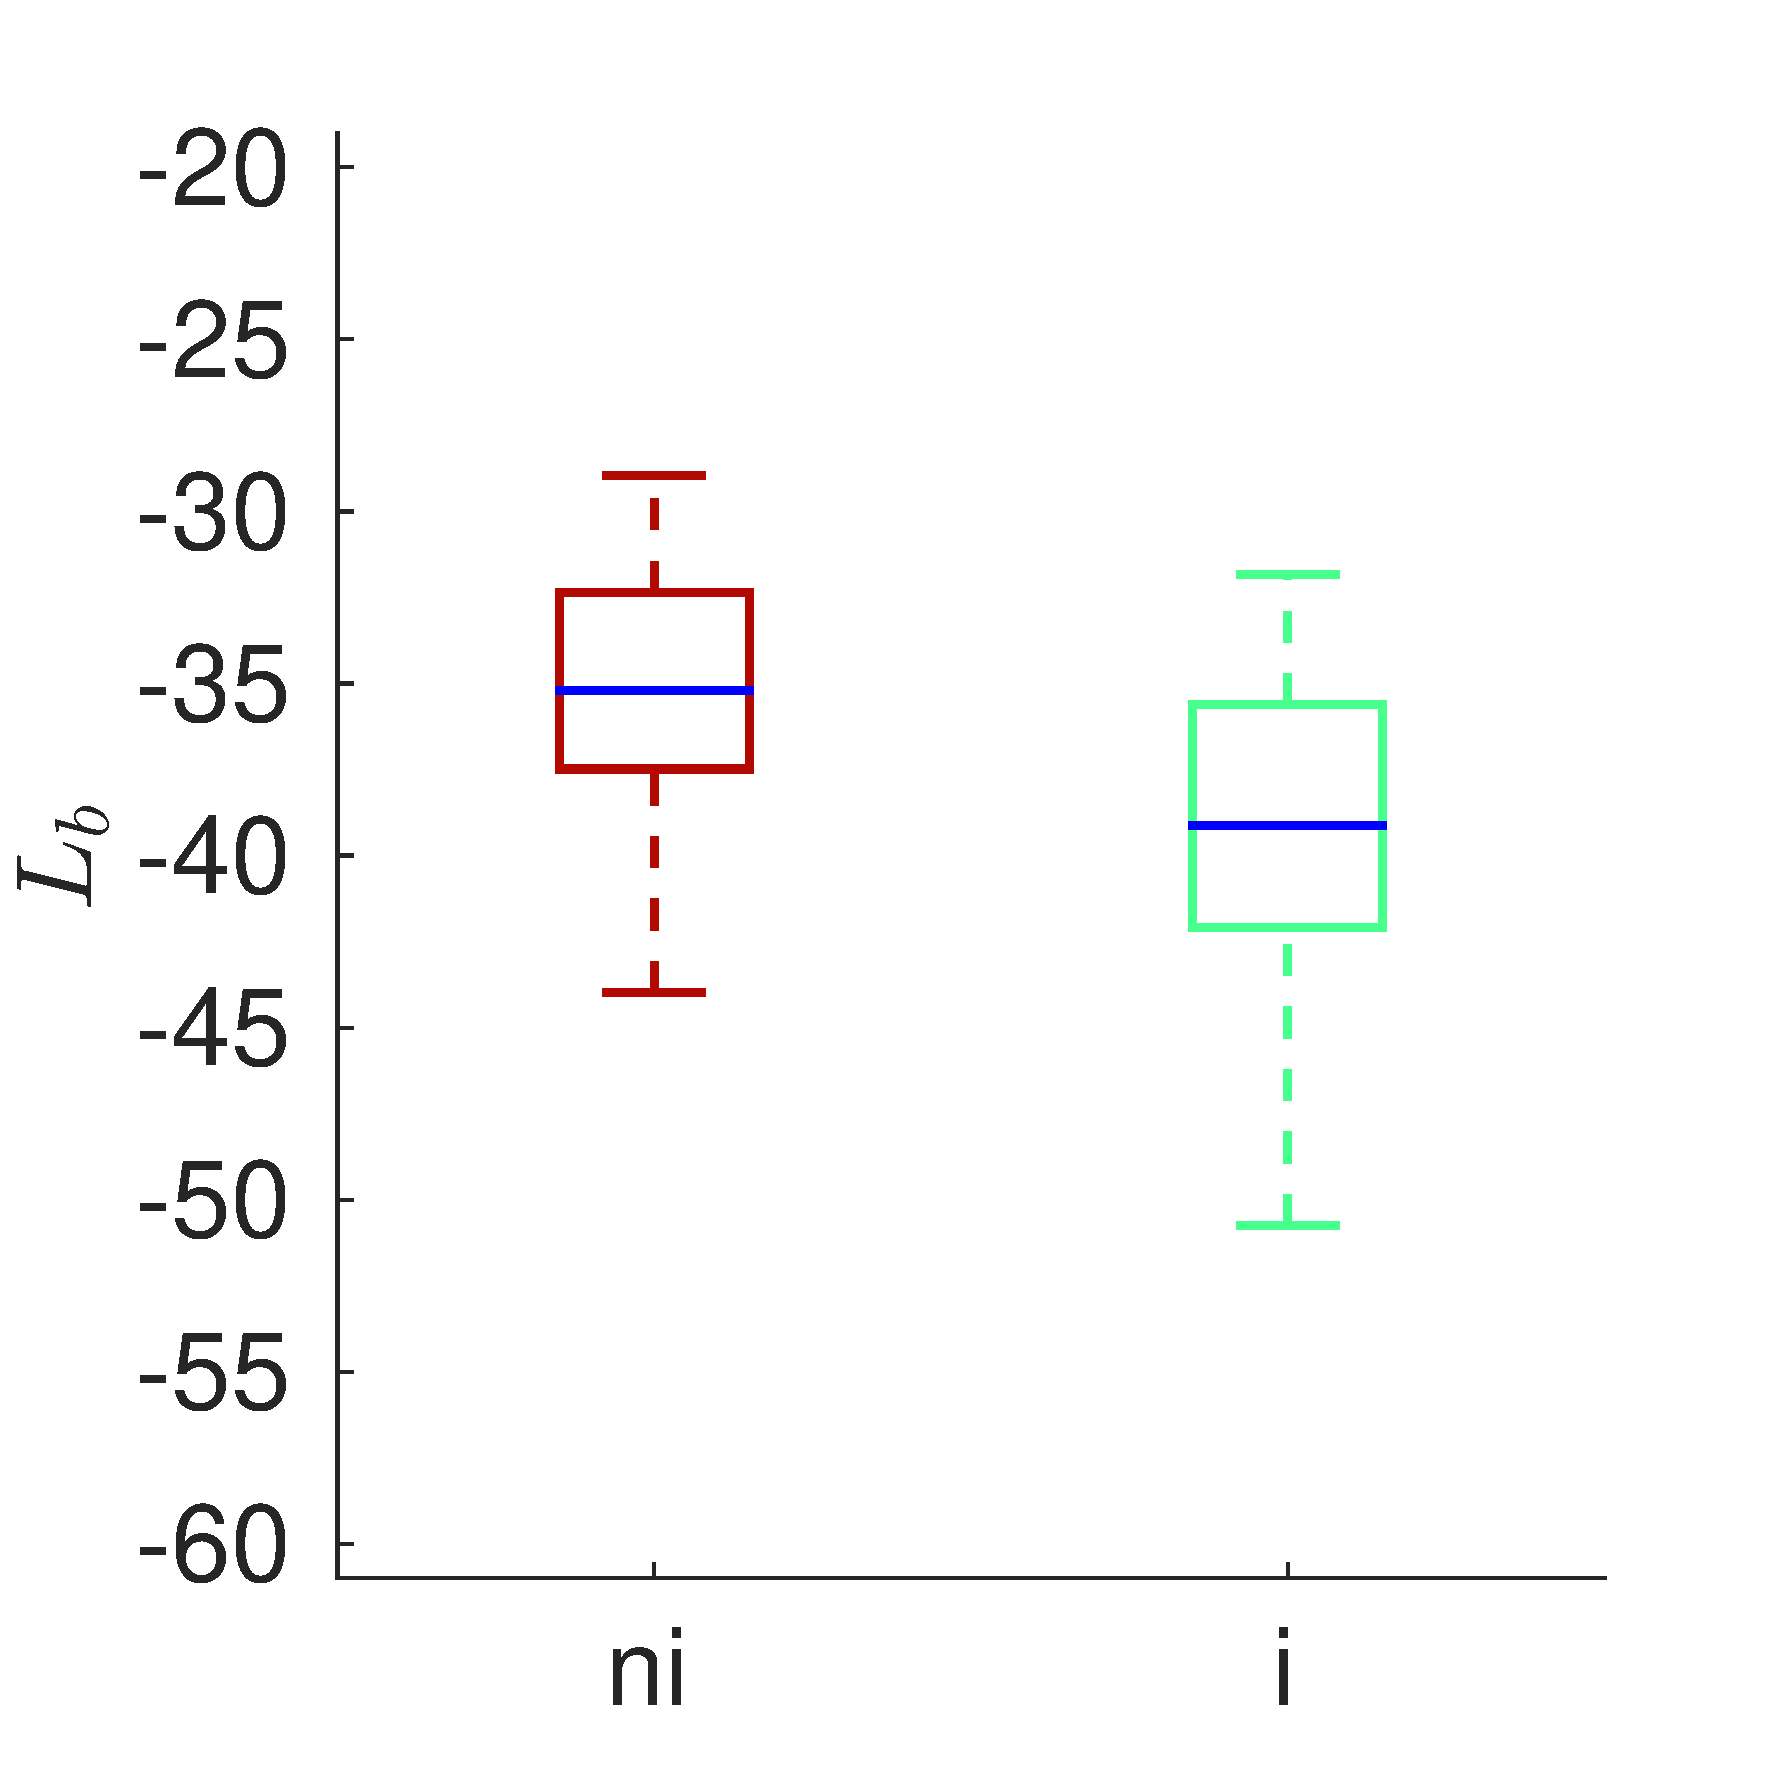
\includegraphics[width=.33\linewidth]{gfx/ch_5/xp_soundlevel_9}\label{fig:soundlevelNoisea}}
        \subfloat[]
        {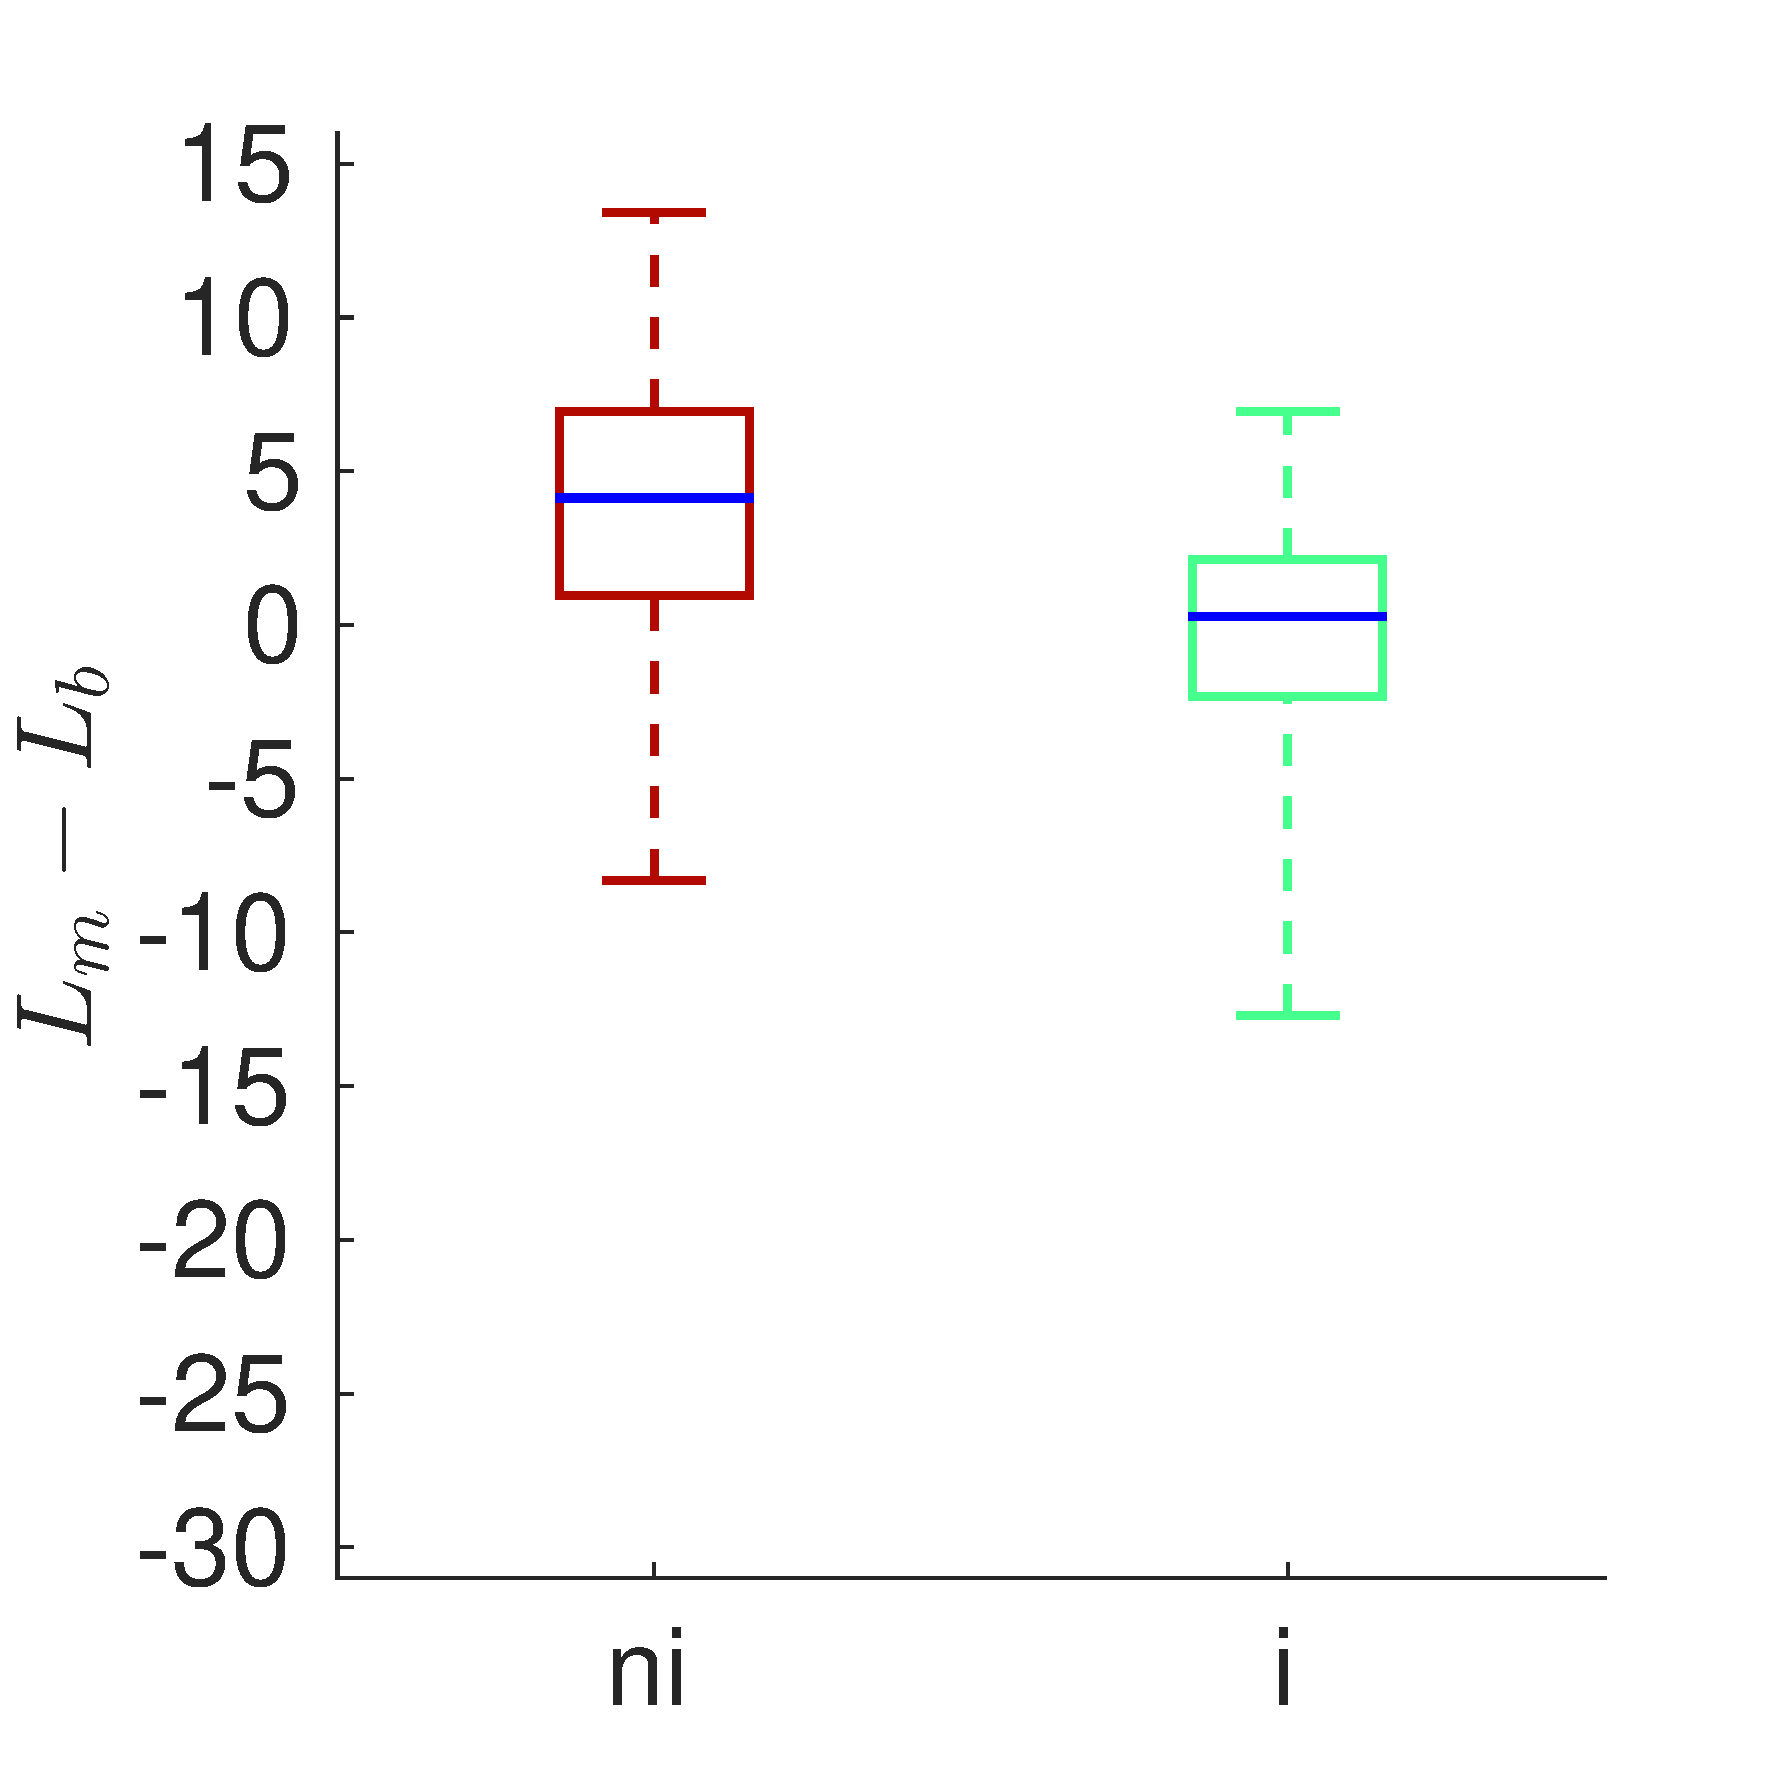
\includegraphics[width=.33\linewidth]{gfx/ch_5/xp_soundlevel_19}\label{fig:soundlevelMarkerDiffa}}\par
        \subfloat[]
        {\includegraphics[width=.33\linewidth]{gfx/ch_5/xp_soundlevel_8}\label{fig:soundlevelMarkerd}}
        \subfloat[]
        {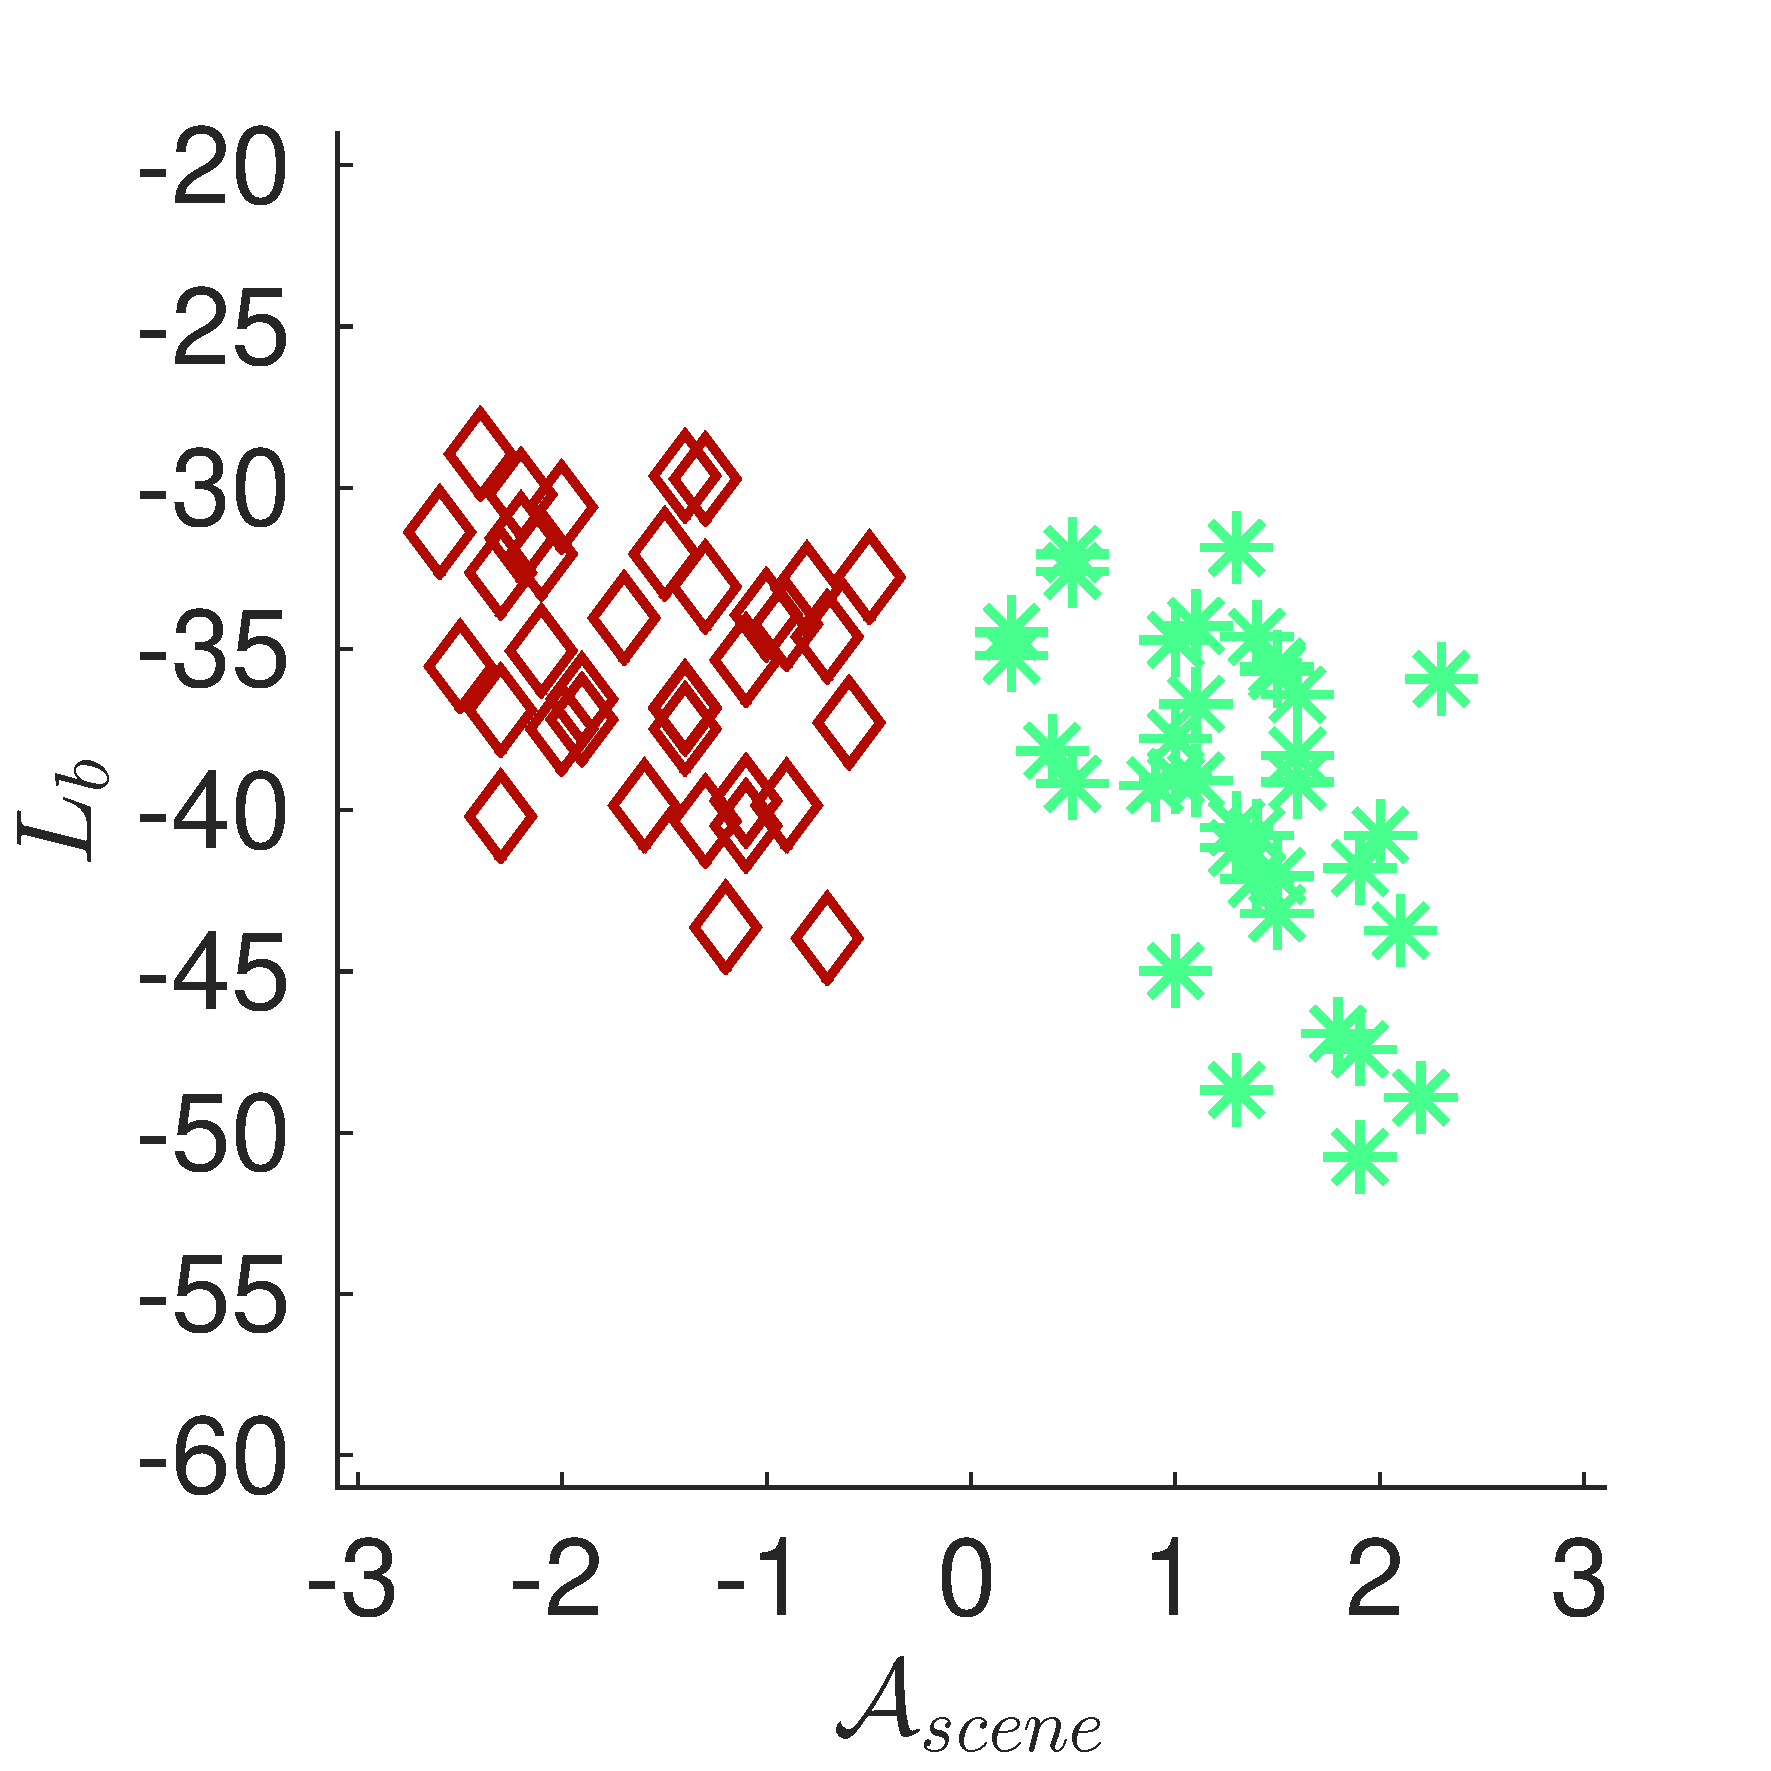
\includegraphics[width=.33\linewidth]{gfx/ch_5/xp_soundlevel_10}\label{fig:soundlevelNoised}}
        \subfloat[]
        {\includegraphics[width=.33\linewidth]{gfx/ch_5/xp_soundlevel_20}\label{fig:soundlevelMarkerDiffd}}
        \caption{Dispersions des descripteurs structurels de niveaux sonores relatifs à la présence des marqueurs $L_m$ (a, d), $L(E)_m$ (b, e) et $L(T)_m$ (c, f), en fonction du type de scènes (a, b, c) et de l'agrément perçu $\mathcal{A}_{scene}$ de l'expérience 1.b (d, e, f).}\label{fig:soundlevelMarker}
\end{figure}

\subsection{Discussions}

De cette analyse, nous retenons les points suivants:

\begin{itemize}
\item \emph{distinguer les i- et ni-scènes}: les descripteurs sémantiques, ainsi que les descripteurs structurels globaux ($L$, $L(E)$ et $L(T)$), permettent de faire la distinction entre les i-scènes et les ni-scènes. La description sémantique semble être plus performante;
\item \emph{événements ou textures}: que ce soit pour les descripteurs sémantiques ou structurels, ce sont majoritairement les événements qui permettent de distinguer les deux types d'environnement, les textures n'apportant, au mieux, qu'une information limitée;
\item \emph{prédire l'agrément}: si l'on considère les corrélations entre les descripteurs structurels et l'agrément, il semble que la manière de percevoir la qualité de l'environnement diffère en fonction de la nature de ce dernier (i ou ni). Il n'apparaît pas envisageable de considérer un même jeu de descripteurs pour prédire, à la fois, l'agrément des i-scènes, et l'agrément des ni-scènes :

\begin{itemize}

\item \emph{pour les ni-scènes}, ce sont le niveau global ($L$ et $L(E)$), ou le niveau des marqueurs sonores ($L_m$ et $L(E)_{m}$), qui impactent négativement l'agrément. On note ici que prendre en compte les contributions de différentes sources n'améliore pas la capacité de prédiction de l'agrément, par rapport à une analyse holistique de l'environnement.

\item \emph{pour les i-scènes}, par contre, prédire l'agrément requiert d'étudier, de manière séparée, les caractéristiques des marqueurs sonores, et celles de l'ensemble des autres sons. Ainsi, le niveau des marqueurs pris relativement au bruit ($L(E)_m-L(E)_b$ et $L_m-L_b$) est positivement corrélé à l'agrément, alors que le niveau du bruit ($L_b$ et $L(E)_b$) est, lui, négativement corrélé.
\end{itemize}
\end{itemize}

Le fait que l'agrément des i-scènes ne se corrèle pas avec des descripteurs physiques holistiques, contrairement à l'agrément des ni-scènes, a récemment été déjà observé \cite{gozalo2015relationship}.

L'existence de deux modes de perception, mobilisant différents types de descripteurs, et dépendant de la nature (dans notre cas hédonique) des stimuli, est un phénomène qui se rapproche de celui observé pour la perception des textures (\cf~Section~\ref{sec:simscene_sampleDataSet}). Le cerveau adapte sa manière de traiter l'information (résumé statistique pour les textures, description fine pour les événements) suite à une prise de décision antérieure quant à la nature du stimulus (à savoir «~est-ce un événement ou une texture ?~»). De la même manière, les indicateurs actifs dans le jugement de l'agrément dépendent, eux aussi, d'une identification préalable de la nature hédonique globale de l'environnement (idéale ou non idéale).

%%%%%%%%%%%%%%%%%%%%%%%%%%%%%%%%%%%%%%%%%%%%%%%%%%%%%%%%%%%%%%%%%%%%%%%
%%%%%%%%%%%%%%%%%%%%%%%%%%% XP 2 %%%%%%%%%%%%%%%%%%%%%%%%%%%%%%%%%%%%%%
%%%%%%%%%%%%%%%%%%%%%%%%%%%%%%%%%%%%%%%%%%%%%%%%%%%%%%%%%%%%%%%%%%%%%%%

\section{Expérience 2 : modification de la composition sémantique}
\label{sec:xp3}

\subsection{Objectif}

L'expérience précédente a montré que, parmi les classes de sons peuplant le monde sonore, celles regroupant les marqueurs sont caractéristiques de certains types d'environnement. Ces marqueurs sonores semblent avoir un impact particulier sur la perception de leurs environnements. C'est ce dernier point qui est étudié dans cette expérience.

Afin de vérifier que l'agrément des scènes idéales et non-idéales dépend de la présence des marqueurs, les scènes sonores précédemment simulées sont régénérées, sans les classes de marqueurs. Pour les i-scènes, les i-marqueurs sont retirés. Pour les ni-scènes, les ni-marqueurs. Une épreuve d'évaluation de l'agrément, dont le protocole se rapproche de celui de l'expérience 1.b, est alors conduite.

L'objectif est de vérifier si l'absence des marqueurs a un impact sur l'agrément perçu. Deux hypothèses sont formulées:

\begin{itemize}
\item \emph{pour les ni-scènes} nous faisons l'hypothèse que l'absence des ni-marqueurs va \textbf{augmenter} la valeur de l'agrément perçu;
\item \emph{pour les i-scènes} nous faisons l'hypothèse que l'absence des i-marqueurs va \textbf{diminuer} la valeur de l'agrément perçu.
\end{itemize}

Si la première hypothèse est intuitive, la deuxième l'est moins. En effet, il n’apparaît pas évident que la suppression des i-marqueurs, bien que s'agissant de sons positivement connotés, diminue la qualité globale d'un environnement. Cette suppression aura, de surcroît, pour effet de diminuer le niveau sonore global de la scène.

Néanmoins, comme nous l'avons vu, le niveau global n'est qu'un indicateur partiel de l'agrément pour les environnements sonores idéaux. Qui plus est, cet indicateur, lorsque qu'il décrit le niveau des i-marqueurs, impacte de manière positive la qualité de la scène. L'hypothèse mérite donc d'être vérifiée.

\subsection{Planification de l'expérience 2}

\subsubsection*{Stimuli}

La banque de données de stimuli compte 144 séquences de 30 secondes. Ces 144 séquences comprennent:

\begin{itemize}
\item \emph{72 am-scènes}: les 72 scènes précédemment simulées, avec les classes de marqueurs (am). Nous notons i/am-scènes, les 36 scènes idéales avec marqueurs, et ni/am-scènes les 36 scènes non-idéales avec marqueurs;
\item \emph{72 sm-scènes}: les 72 scènes précédemment simulées, régénérées sans les classes de marqueurs (sm). Nous notons i/sm-scènes, les 36 scènes idéales sans marqueurs, et ni/sm-scènes les 36 scènes non-idéales sans marqueurs.
\end{itemize}

Nonobstant l'absence des marqueurs, les am- et sm-scènes sont en tout point semblables.

Nombre de am-scènes sont composées, en majorité, de samples de marqueurs. Afin de ne pas dénaturer abusivement ces scènes, en créant notamment des temps de «~vide~», \ie~ne comprenant aucun sample, nous ne supprimons que les marqueurs des classes d'événements du premier niveau d'abstraction (\cf~Tableau~\ref{tab:markers}). Ces classes sont:

\begin{itemize}
\item \emph{cloche}, \emph{sonnette de vélo}, \emph{animaux} pour les i/sm-scènes;
\item \emph{sirène}, \emph{klaxon} pour les ni/sm-scènes.
\end{itemize}

Il est important de noter ici que tous les i- et ni-marqueurs ne sont donc pas supprimés dans les sm-scènes.

\subsubsection*{Procédure}

Les sujets évaluent les 144 scènes. L'évaluation s'effectue sur une échelle sémantique bipolaire de 11 points allant de -5 (non-idéale/très désagréable) à +5 (idéale/très agréable). Avant de noter une scène, les sujets doivent obligatoirement en écouter les 20 premières secondes. Après la notation, ils sont libres de passer à la scène suivante.

Pour chaque sujet, les scènes sont présentées dans un ordre aléatoire. Les 10 premières scènes permettent au sujet de calibrer ses notes. Elles sont obligatoirement composées de 5 i/am-scènes et de 5 ni/am-scènes. Ces 10 premières scènes sont rejouées à la fin de l'expérience, et seules les notes données à la deuxième occurrence sont prises en compte.

L'expérience est prévue pour durer 1 heure. Les sujets ne connaissent pas la nature des scènes.

\subsubsection*{Dispositif expérimental}

Tous les sujets passent l'expérience sur des machines identiques. L'audio est diffusé en monophonie, par le biais de casques audio semi-ouverts \emph{Beyer-Dynamic DT 990 Pro}. Toutes les scènes sonores ont été re-simulées sur la base des partitions obtenues lors de l'expérience de simulation. Le niveau sonore de sortie est identique pour tous les sujets.

Tous les sujets réalisent l'expérience simultanément, dans un environnement calme. Ils n'ont pas le droit de s'adresser la parole pendant l'expérience.

Un expérimentateur est présent durant la totalité de l'expérience, afin de contrôler le bon déroulement de cette dernière, et de répondre aux éventuelles questions des sujets.

\subsubsection*{Participants}

12 sujets (4 femmes) participent à l'expérience. Aucun d'entre eux n'a réalisé l'expérience de simulation, ni la première expérience d'évaluation. Les sujets sont âgés de 22 à 61 ans (moyenne: 29.5, écart-type: 14). Tous les sujets vivent dans un milieu urbain.

Tous les sujets ont réalisé l'expérience avec succès.

\subsection{Données et méthodes d'analyses}

Les données analysées sont les mêmes que pour la première expérience. Nous invitons le lecteur à se référer à la section~\ref{sec:xp1_dataAna} pour plus de détails.

Il s'agit ici de vérifier que la suppression des i- et ni-marqueurs impacte l'agrément perçu. Pour ce faire, nous utilisons l'analyse de variance. Nous considérons, comme variable dépendante, $\mathcal{A}_{sujet}$, et, comme variables indépendantes, le type d'environnement (i/ni), et la présence/absence de marqueurs (am/sm). Chaque sujet devant évaluer la totalité des stimuli, une ANOVA à mesures répétées à deux facteurs est utilisée afin vérifier s'il existe des différences significatives d'agrément perçu. Les deux variables indépendantes sont considérées comme des facteurs intra-sujet (\emph{within-subject}. Les facteurs n'étant composés que de deux niveaux chacun (type: i/ni; marqueur: am/sm), l'hypothèse de sphéricité n'a pas besoin d'être vérifiée. Les analyses \emph{post hoc} sont conduites en appliquant la procédure de Tukey-Kramer.

Tous les tests de significativité sont effectués avec un seuil critique $\alpha=0.05$.

\subsection{Résultats}

\subsubsection{Détection des valeurs extrêmes}

Considérons $\mathcal{A}_{sujet}$ pour les am-scènes. Il apparaît que les réponses d'un des sujets diffèrent des autres. Ce dernier a évalué positivement près de la moitié des ni/am-scènes (\cf~Annexe~\ref{app:xp2} : sujet 7). Le sujet a donné à 58\% des ni/am-scènes une note supérieure à 0, contre une moyenne de 11\% pour les autres sujets. De plus, le sujet a utilisé l'ambitus maximal (-5 à 5) pour noter à la fois les i/ et ni/am-scènes. Ces faits n'ayant pas été observés pour les autres sujets, que l'on considère les expériences 2 ou 1.b, le sujet 7 est éliminé de l'analyse.

\subsubsection{Influence de la présence des marqueurs sur l'agrément perçu}


Dans cette section nous étudions comment les sujets ont perçu les différents types de scènes, nommément: i/am-, ni/am-, i/sm- et ni/sm-scène. L'ANOVA à mesures répétées pratiquée sur $\mathcal{A}_{sujet}$ montre un effet significatif du type d'environnement (i/ni: $F[1,10]=175$, $p<0.01$), de la présence/absence des marqueurs (am/sm: $F[1,10]=7$, $p<0.05$), ainsi que de l'interaction entre les deux facteurs ($F[1,10]=67$, $p<0.01$).

L'analyse \emph{post hoc} montre, quant à elle, des différences significatives entre tous les groupes d'observations, notamment entre les i/am- et i/sm-scenes ($p<0.05$) et les ni/am- et ni/sm-scenes ($p<0.01$).

Ces résultats indiquent que la suppression des événements a effectivement modifié la perception des scènes par les sujets. Nos deux hypothèses sont ainsi vérifiées:

\begin{itemize}
\item la suppression des ni-marqueurs a amélioré les qualités perçues des ni-scènes;
\item la suppression des i-marqueurs a diminué les qualités perçues des i-scènes.
\end{itemize}

L'interaction significative montre que l'effet du type d'environnement influe sur l'effet de l'absence/présence des marqueurs. En effet la moyenne des écarts entre am- et sm-scènes est plus importante pour les ni-scènes ($1.1$) que pour les i-scènes ($0.5$).

\subsection{Discussions}

Cette expérience fait apparaître que la présence, dans une scène, des marqueurs relevés à l'expérience 1 impacte bien l'agrément perçu. La suppression des ni-marqueurs a un effet bénéfique sur le ressenti, tandis que, plus surprenant, la suppression des i-marqueurs dégrade légèrement la qualité. Ce dernier point est d'autant plus marquant que, du fait de la suppression des marqueurs, le niveau des i/am-scènes est supérieur à celui des i/sm-scènes.

Les i-marqueurs ont donc bien un effet bénéfique sur la perception d'un environnement. Le fait que leur suppression diminue $\mathcal{A}_{scene}$ montre clairement qu'il est possible d'améliorer la qualité sonore d'un lieu en ajoutant des sons bien acceptés comme \emph{oiseau}. Ces conclusions vont dans le sens de l'approche positive introduite par Schafer \cite{schafer1977tuning}.


%%%%%%%%%%%%%%%%%%%%%%%%%%%%%%%%%%%%%%%%%%%%%%%%%%%%%%%%%%%%
%%%%%%%%    DISCUSSION AND PERSPECTIVES   %%%%%%%%%%%%%%%%%%
%%%%%%%%%%%%%%%%%%%%%%%%%%%%%%%%%%%%%%%%%%%%%%%%%%%%%%%%%%%%


\section{Conclusions et perspectives}

Les expériences ont montré que la majorité des descripteurs utilisés, qu'ils soient sémantiques ou structurels, permettent de faire la distinction entre une scène idéale et une scène non-idéale.

Cependant, nous observons que les caractéristiques physiques corrélées à l'agrément diffèrent clairement suivant la nature hédonique des scènes. Dans le cas des scènes idéales, c'est avant tout l'émergence de marqueurs sonores qui détermine la qualité perçue, alors que dans le cas des scènes non-idéales, c'est le niveau sonore global qui influe sur l'agrément.

Ces résultats tendent à confirmer que la perception des qualités d'une scène dépend avant tout des sources sonores qui la composent, les caractéristiques structurelles mobilisées dans le processus perceptif semblant varier d'une source à l'autre, et d'un type d'environnement à l'autre. Ce fait montre qu'il est illusoire d'envisager qu'un descripteur physique holistique puisse rendre compte, de manière pertinente, des qualités affectives de tous types d'environnement.

Cet état de fait peut potentiellement influer sur les stratégies à adopter pour améliorer la qualité de l’environnement sonore:

\begin{itemize}
\item dans le cadre de scènes non-idéales, il s'agit de diminuer le niveau sonore, soit de manière globale, soit en agissant sur certaines sources (\emph{sirène}, \emph{klaxon});
\item dans le cadre de scènes idéales, il s'agit 1) d'identifier les sons agréables, \ie~les marqueurs sonores, 2) de baisser le niveau des autres sons, 3) voire, en restant dans la limite du raisonnable, d'augmenter le niveau des marqueurs par rapport aux autres sons.
\end{itemize}

Ces travaux nous permettent enfin de conjecturer quant à la nature des représentations mentales des concepts «~environnement sonore urbain agréable~» (EA) et «~environnement sonore urbain désagréable~» (ED).

Premièrement, le fait que les informations sémantiques (sources sonores présentes) et structurelles soient différentes pour les scènes idéales et non-idéales nous porte à croire que ces deux types d'informations caractérisent les concepts EA et ED.

Deuxièmement, le fait que la suppression des marqueurs sonores modifie l'agrément perçu nous porte à croire que le concept abstrait lié à l'agrément (\eg. scène agréable) dépend de l'activation d'un réseau de concepts concrets liés aux sources (dans notre cas \emph{oiseau}, \emph{cloche} et \emph{sonnette vélo}).

Troisièmement, le fait que les descripteurs structurels corrélés à l'agrément diffèrent en fonction du type de scènes nous porte à croire que les caractéristiques structurelles permettant de distinguer deux instances d'un même concept abstrait lié à l'agrément ne sont pas les mêmes pour EA et ED.

Au terme de notre étude, nous pensons que la simulation est un outil dont le développement pourrait permettre aux décideurs en matière d'urbanisme d'interroger toute une communauté sur ses représentations propres des environnements sonores auxquels elle est exposée, et, pourquoi pas, sur les représentations des environnements sonores auxquels elle voudrait être exposée.

Dans la continuité des travaux réalisés, il conviendrait de multiplier les expériences de simulation, en faisant varier les qualités affectives (calme, confortable, gênante, \etc), mais aussi en spécifiant des lieux particuliers (parc, place, rue, \etc), afin d'élaborer des corpus entiers de scènes cognitivement renseignées de paysages sonores.

Il serait par ailleurs intéressant d'utiliser la simulation afin d'étudier plus avant les effets provoqués par la modification volontaire d'une caractéristique d'une scène, comme lors de la suppression des marqueurs sonores pratiquée dans l'expérience 2.

Enfin, l'on pourrait encore étudier l'influence des contextes socio-culturels sur la perception. Dans les faits, si le son de cloche est le plus souvent un marqueur d'environnement de qualité pour un occidental, cela ne se vérifie pas nécessairement auprès de sujets de culture orientale, moyen-orientale ou autre.

Outre les possibilités déjà évoquées, la simulation présente encore dans ce cas deux avantages:

\begin{itemize}
\item le simulateur peut être déployé à large échelle via internet;
\item les scènes simulées peuvent être analysées sans avoir à tenir compte des différentes langues maternelles des sujets, la nature sémantique des classes de sons utilisées étant connue \emph{a priori} par l'expérimentateur et sans avoir besoin d'analyser la scène sonore pour idientifier les sources, leurs présences dans la scène étant directement exploitable.
\end{itemize}

Bien évidemment, ces approches nécessitent d'accroître la taille des banques de sons isolés disponibles, un effort conséquent, mais nécessaire, qui contribuera grandement aux nombreux domaines de recherche ayant trait aux scènes sonores.

\section*{\normalsize Acknowledgements}
\setlength{\parindent}{0.7cm}
Research project partly funded by ANR-11-JS03-005-01. The authors would like to thank the students of the Ecole Centrale de Nantes for their willing participation.


%%%%%%%%%%%%%%%%%%%%%%%%%%%%%%%%%%%%%%%%%%%%%%%%%%%%%%%%%%%%
%%%%%%%%%%%%%%%%    Bibliography    %%%%%%%%%%%%%%%%%%%%%%%%
%%%%%%%%%%%%%%%%%%%%%%%%%%%%%%%%%%%%%%%%%%%%%%%%%%%%%%%%%%%%

\References{}{Bibliography}{actalit}

%%%%%%%%%%%%%%%%%%%%%%%%%%%%%%%%%%%%%%%%%%%%%%%%%%%%%%%%%%%%
%%%%%%%%%%%%%%%%%%%    APPENDICES   %%%%%%%%%%%%%%%%%%%%%%%%
%%%%%%%%%%%%%%%%%%%%%%%%%%%%%%%%%%%%%%%%%%%%%%%%%%%%%%%%%%%%

\onecolumn

\appendix
\section{Taxonomies des classes de sons}
\label{app:taxonomie}

\begin{figure}[h]
        \myfloatalign
        \subfloat[]
        {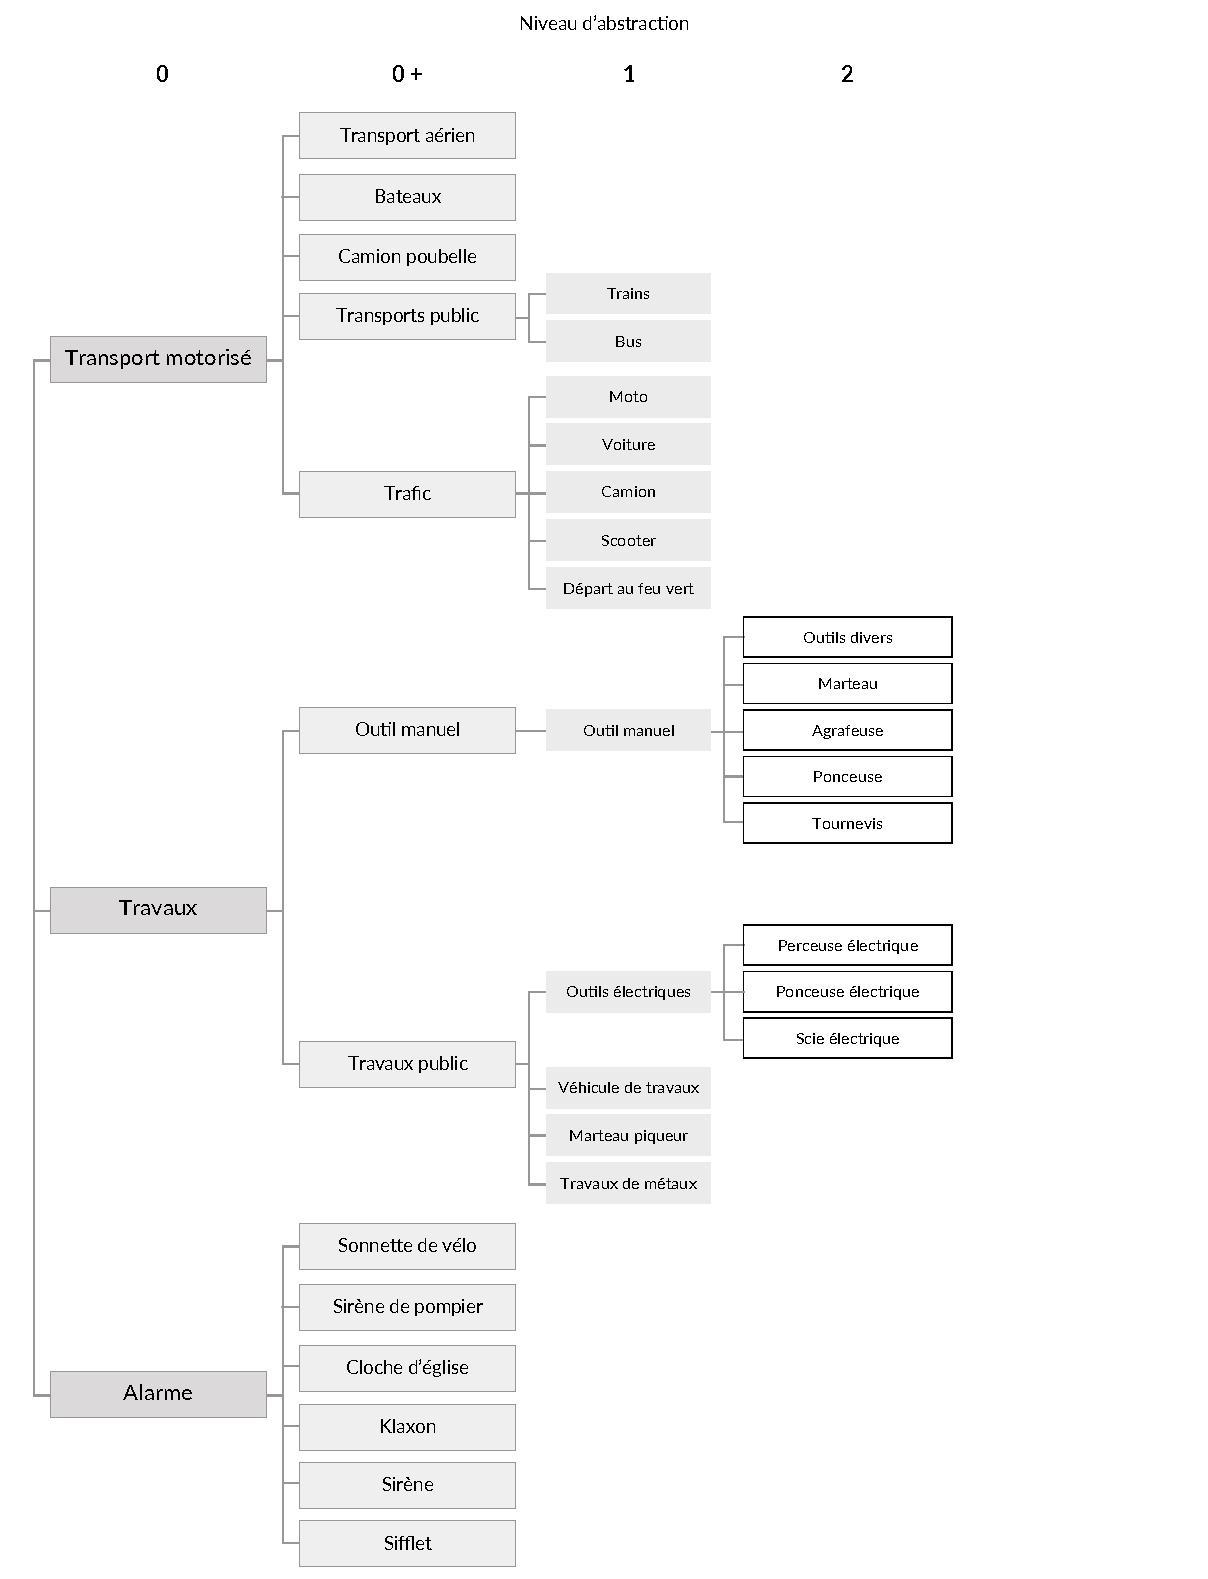
\includegraphics[width=.5\columnwidth]{gfx/ch_5/event_1}\label{fig:taxonomieEventa}}
        \subfloat[]
        {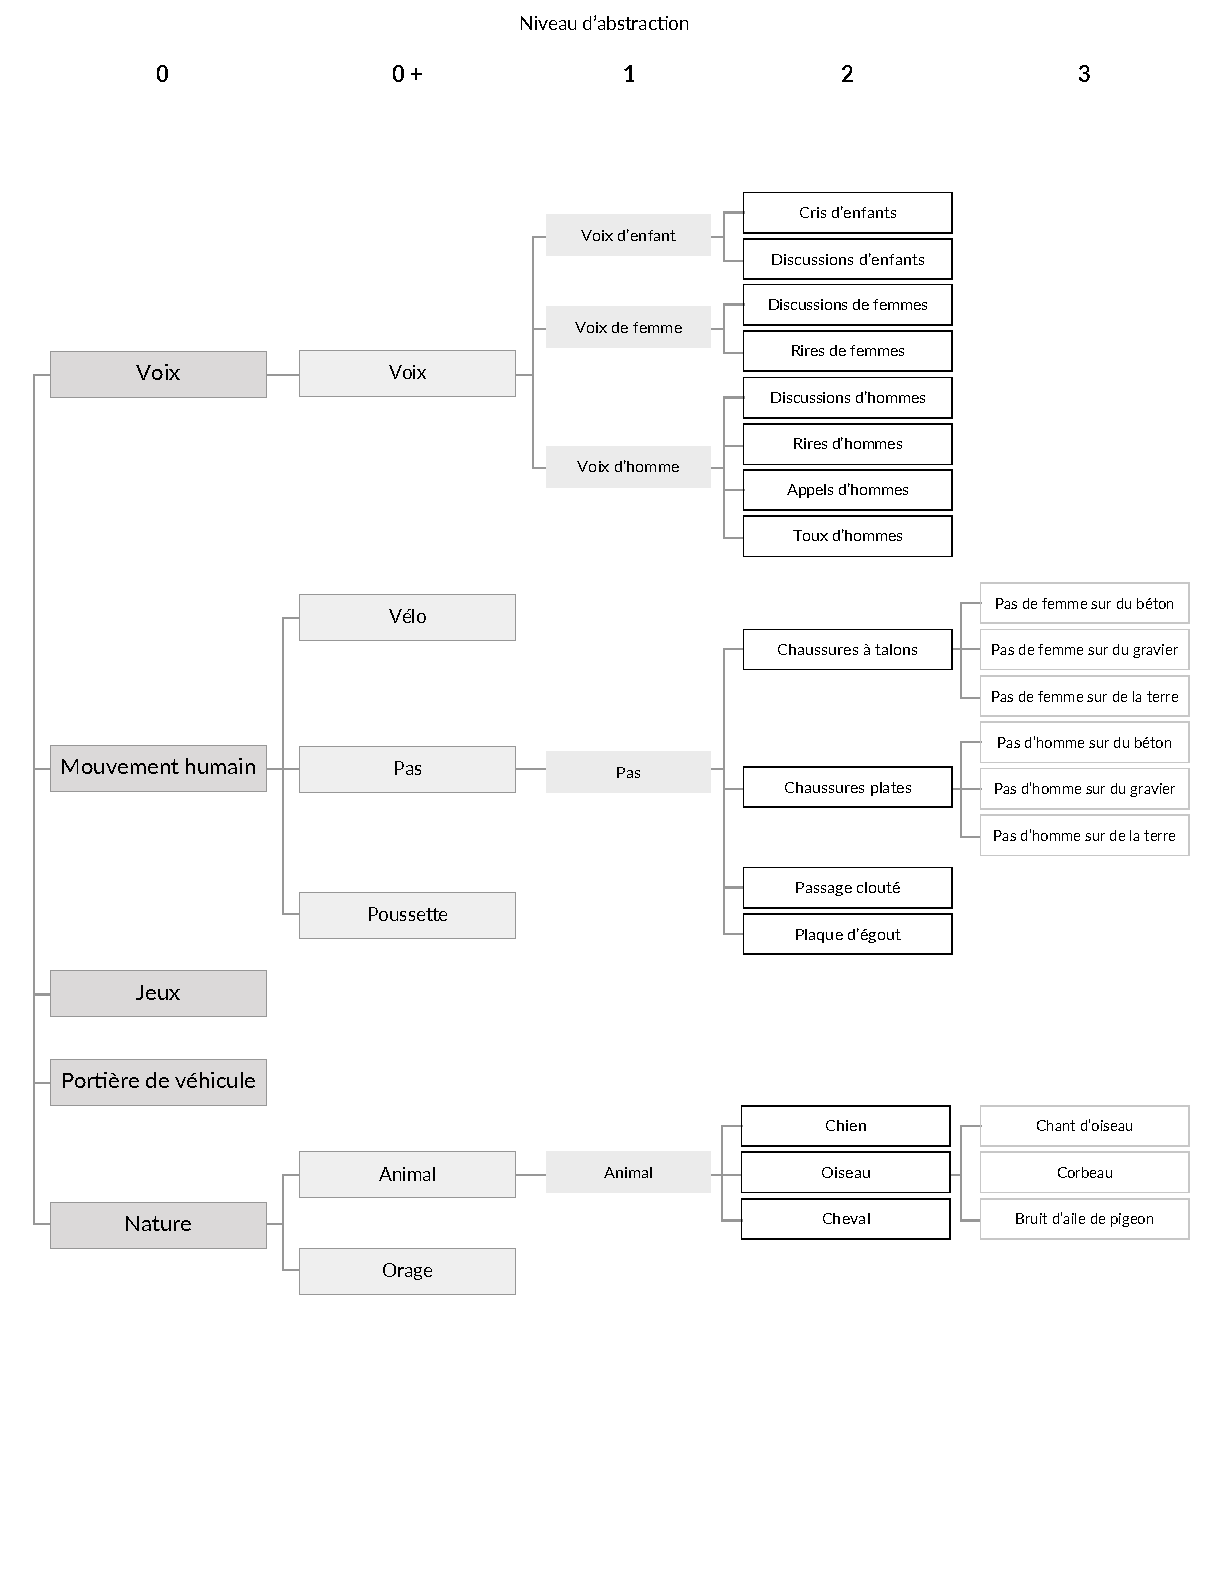
\includegraphics[width=.5\columnwidth]{gfx/ch_5/event_2}\label{fig:taxonomieEventb}}\par
        \subfloat[]
        {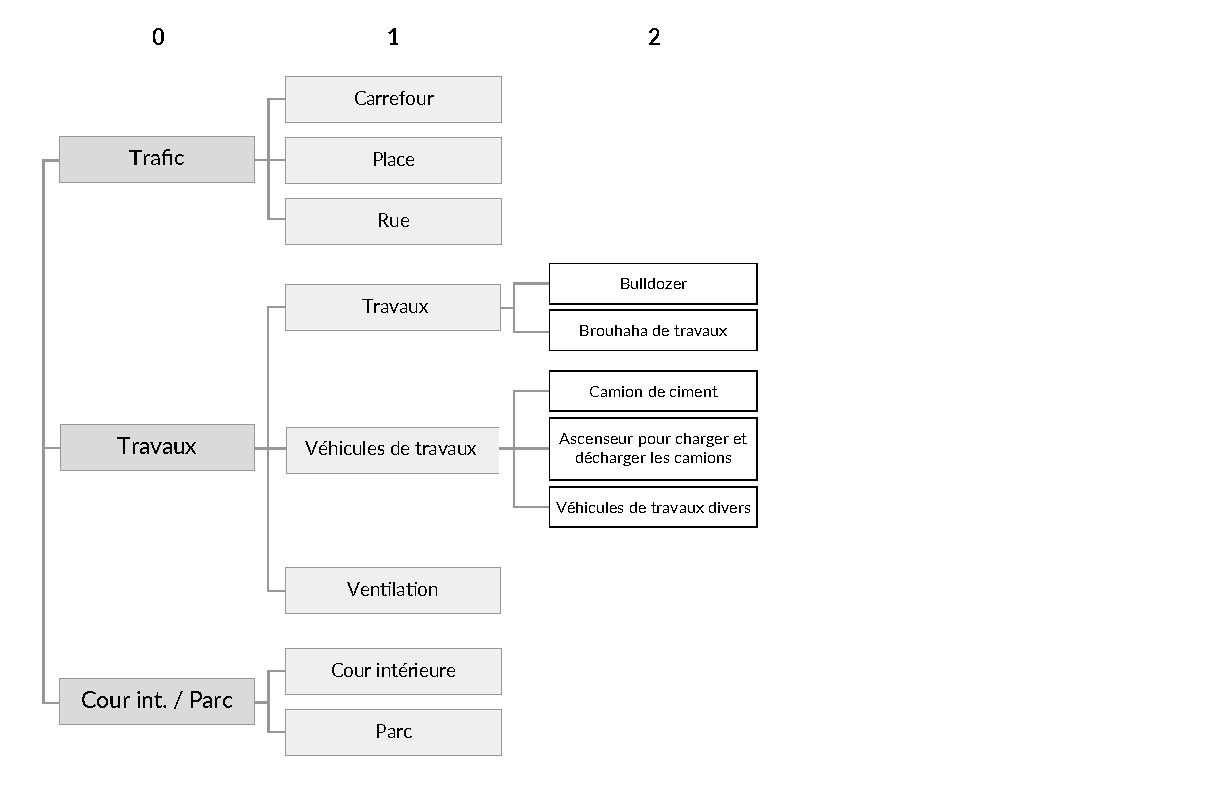
\includegraphics[width=.5\columnwidth]{gfx/ch_5/texture_1}\label{fig:taxonomieTexturea}}
        \subfloat[]
        {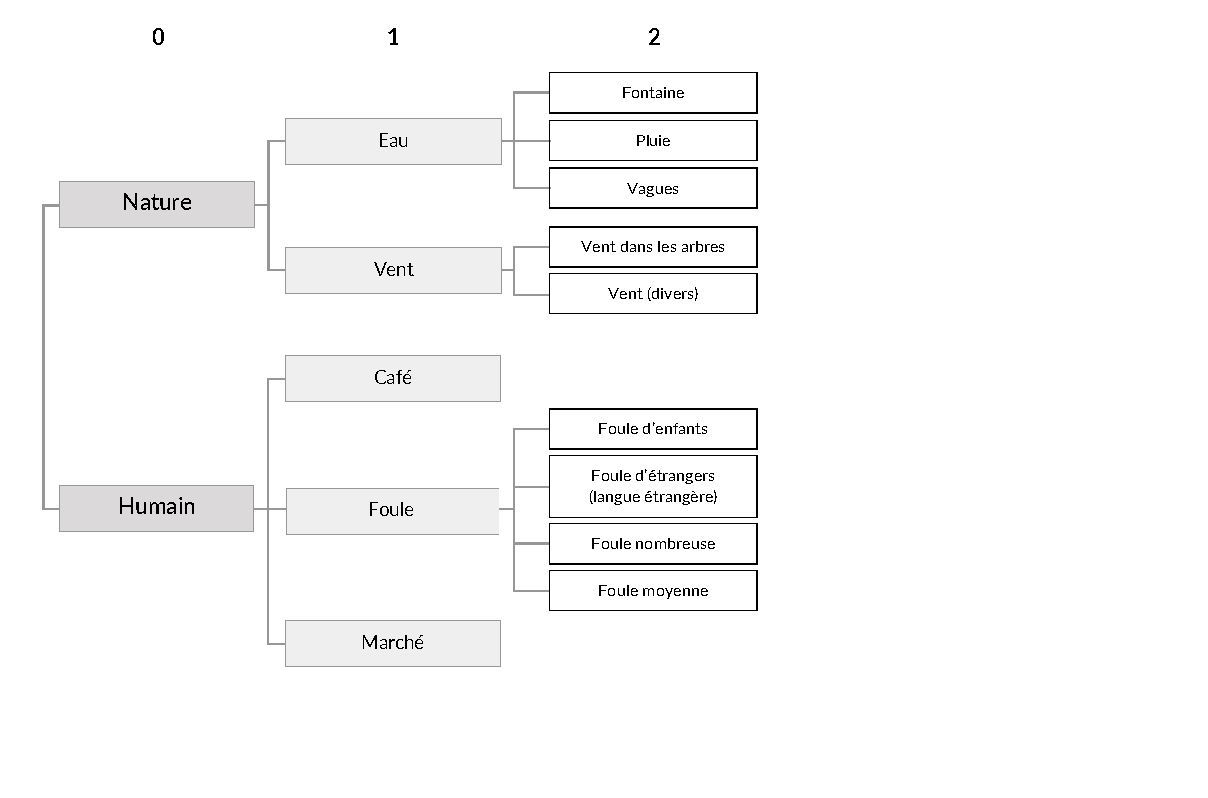
\includegraphics[width=.5\columnwidth]{gfx/ch_5/texture_2}\label{fig:taxonomieTextureb}}
       \caption{Taxonomies des classes de sons utilisées pour la simulation des environnements sonores urbains : (a,b) événements sonores et (c,d) textures sonores.}
       \label{fig:taxonomie}
\end{figure}

\newpage
\section{Dispersions des notes données par les sujets lors de l'expérience 2}
\label{app:xp2}

\begin{figure}[h]
        \myfloatalign
        \subfloat[sujet 1]
        {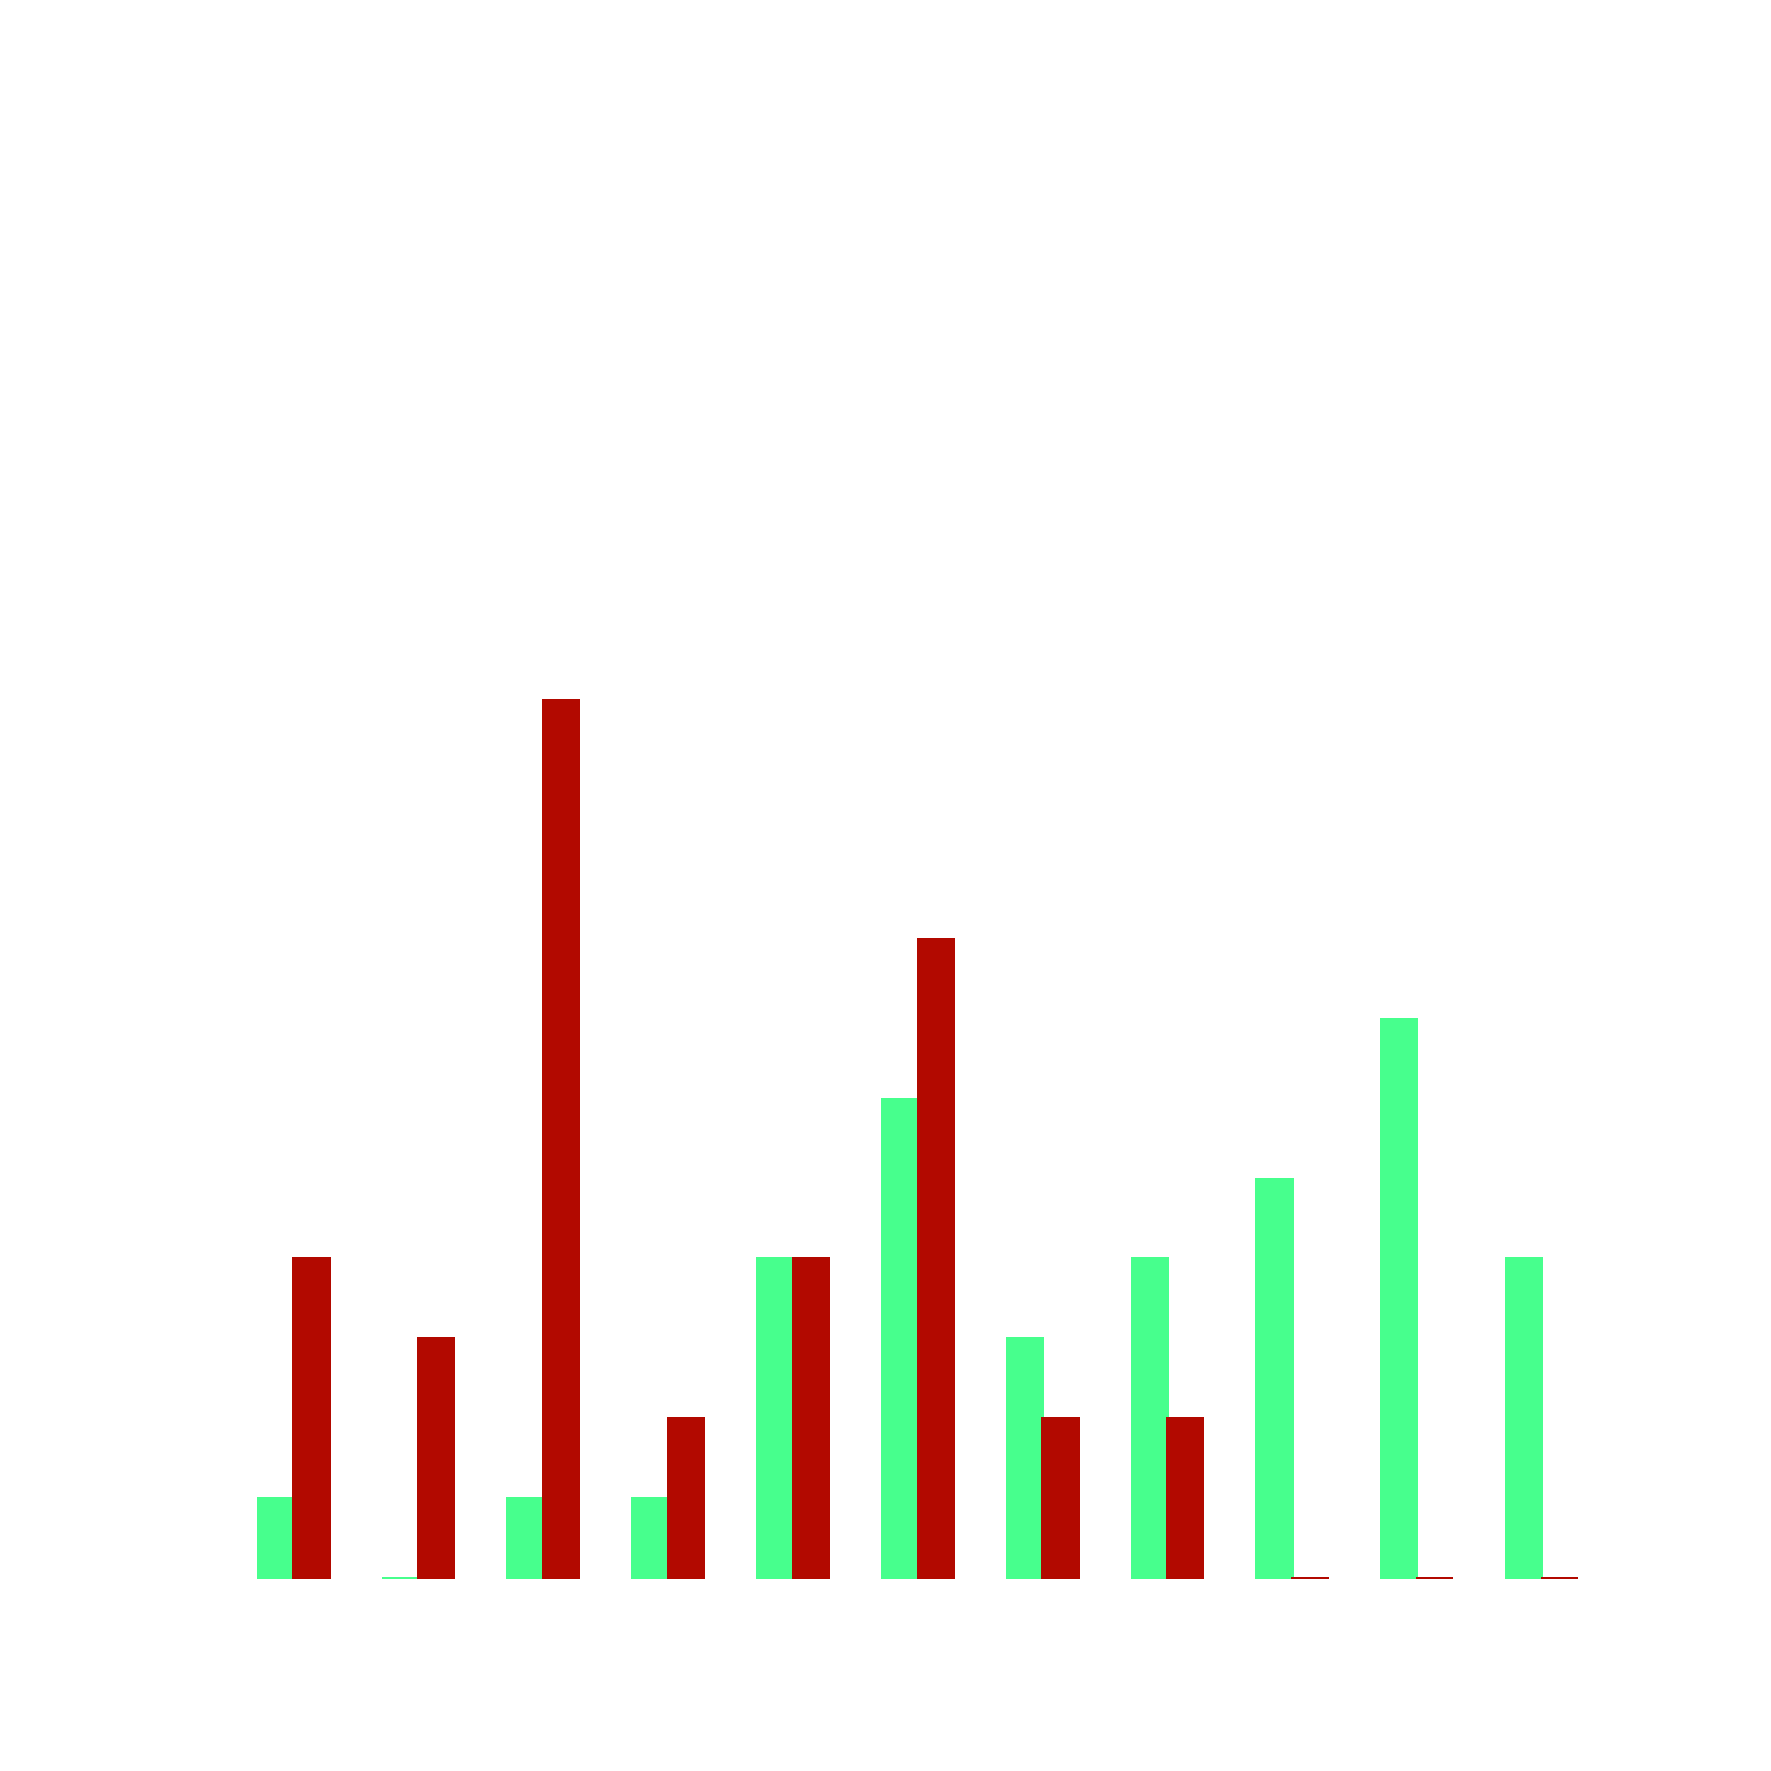
\includegraphics[width=.24\linewidth]{gfx/ch_5/xp4_note_1}\label{fig:xp4_note_1a}}
        \subfloat[sujet 2]
        {\includegraphics[width=.24\linewidth]{gfx/ch_5/xp4_note_2}\label{fig:xp4_note_1b}}
        \subfloat[sujet 3]
        {\includegraphics[width=.24\linewidth]{gfx/ch_5/xp4_note_3}\label{fig:xp4_note_1c}}
        \subfloat[sujet 4]
        {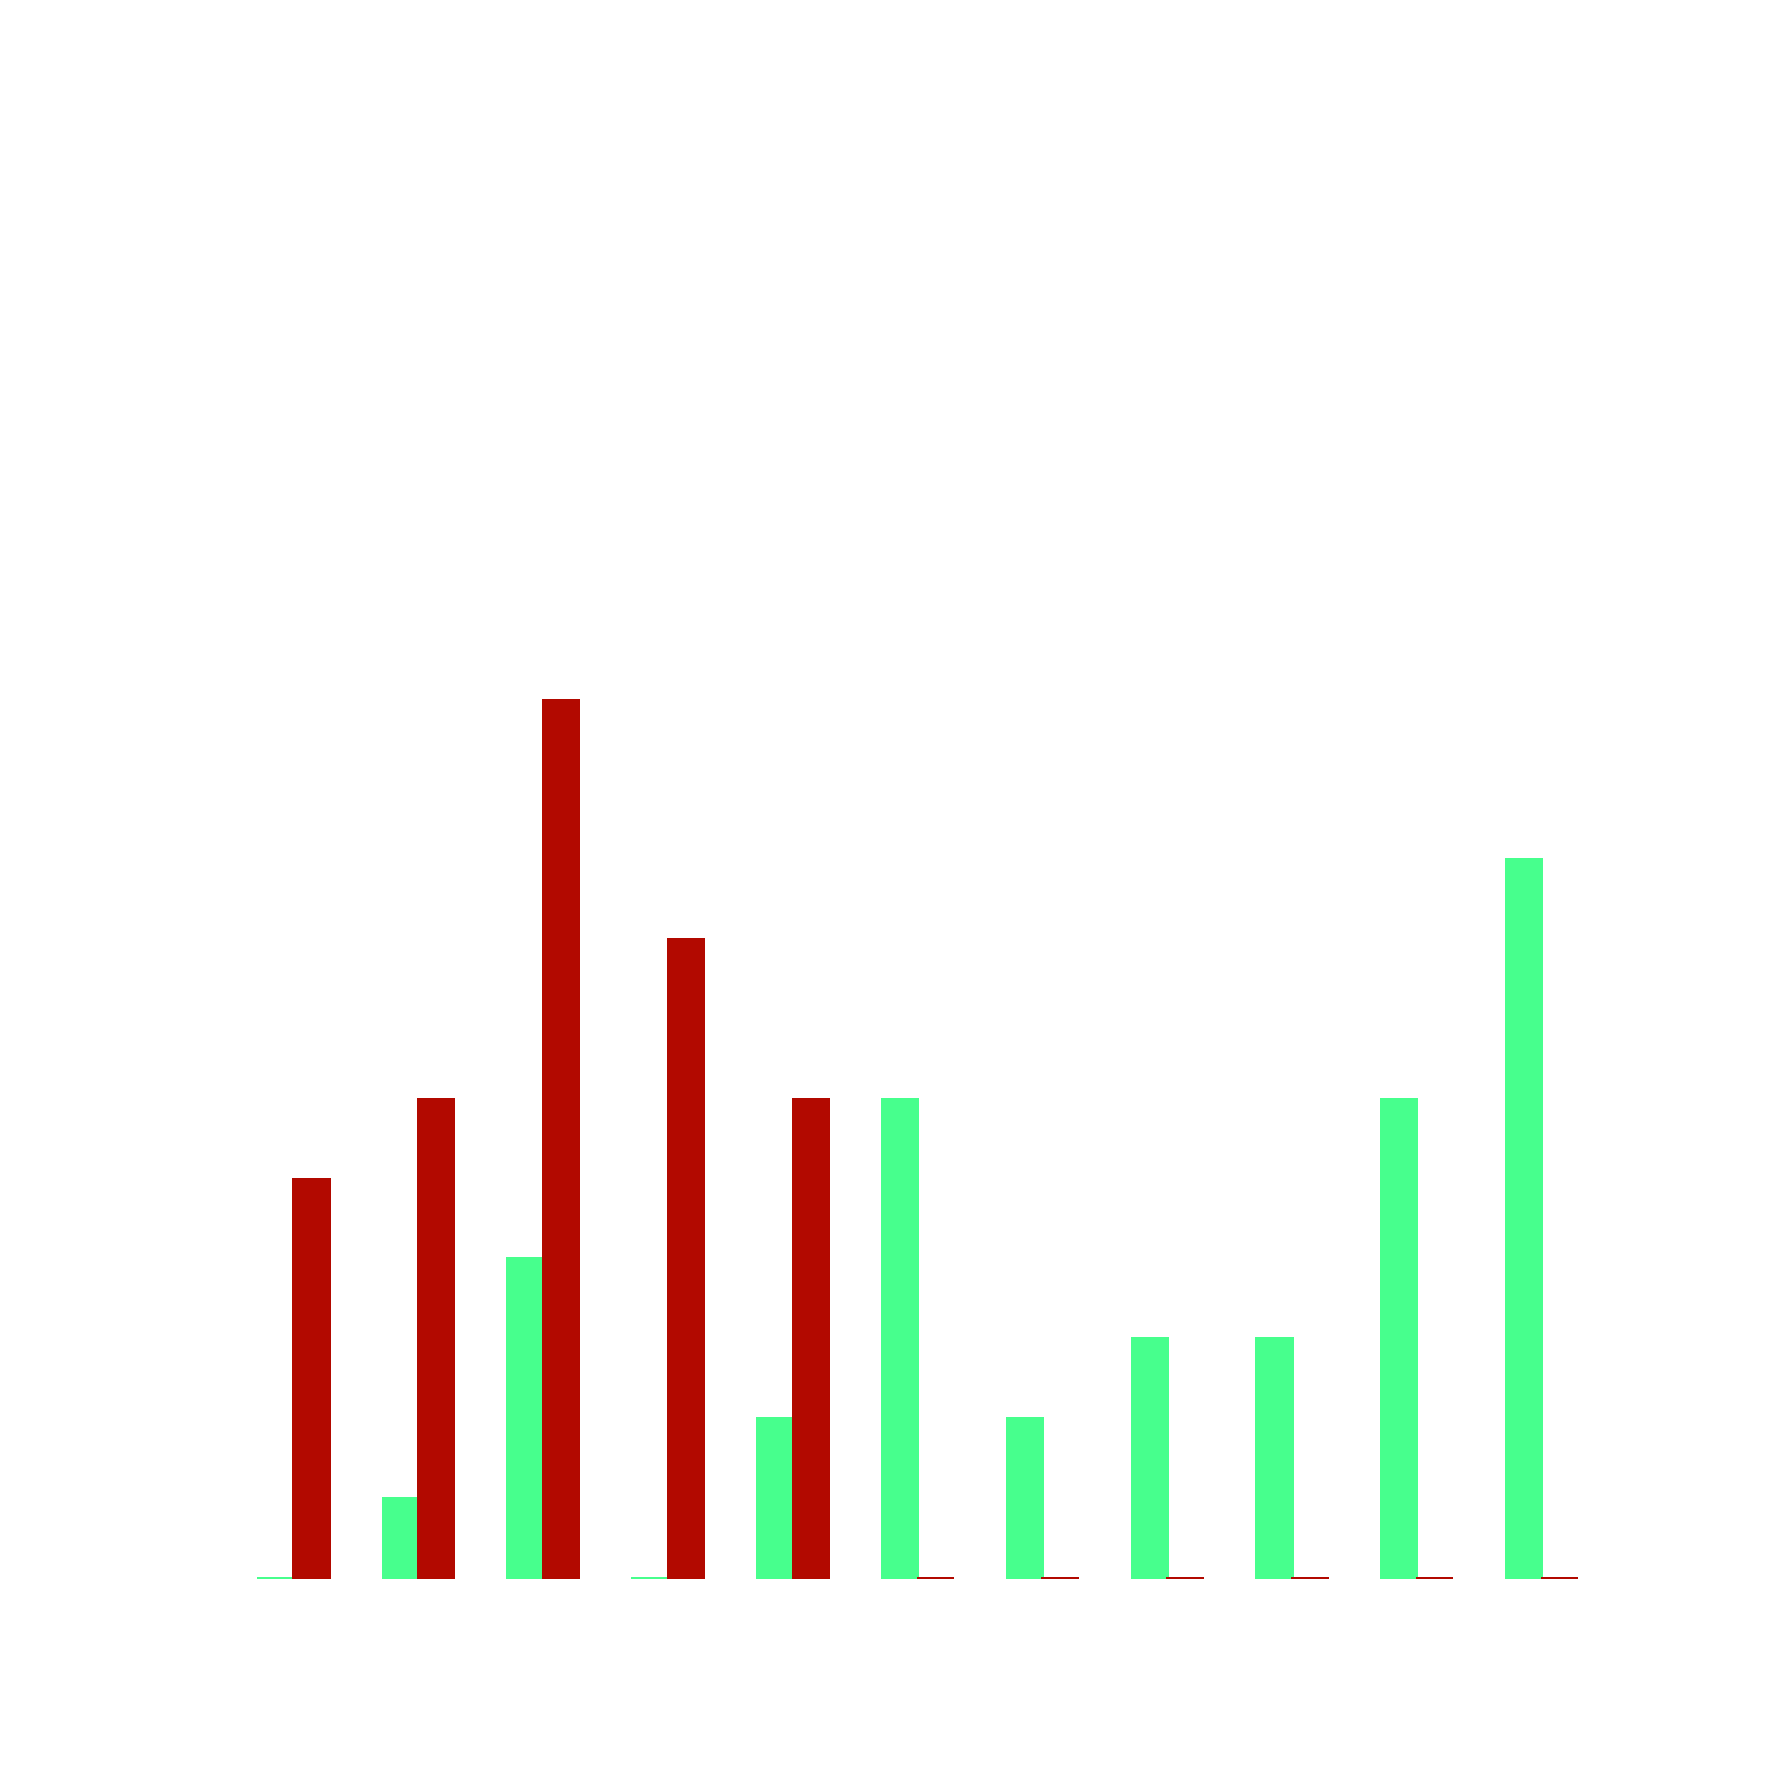
\includegraphics[width=.24\linewidth]{gfx/ch_5/xp4_note_4}\label{fig:xp4_note_1d}} \par
        \subfloat[sujet 5]
        {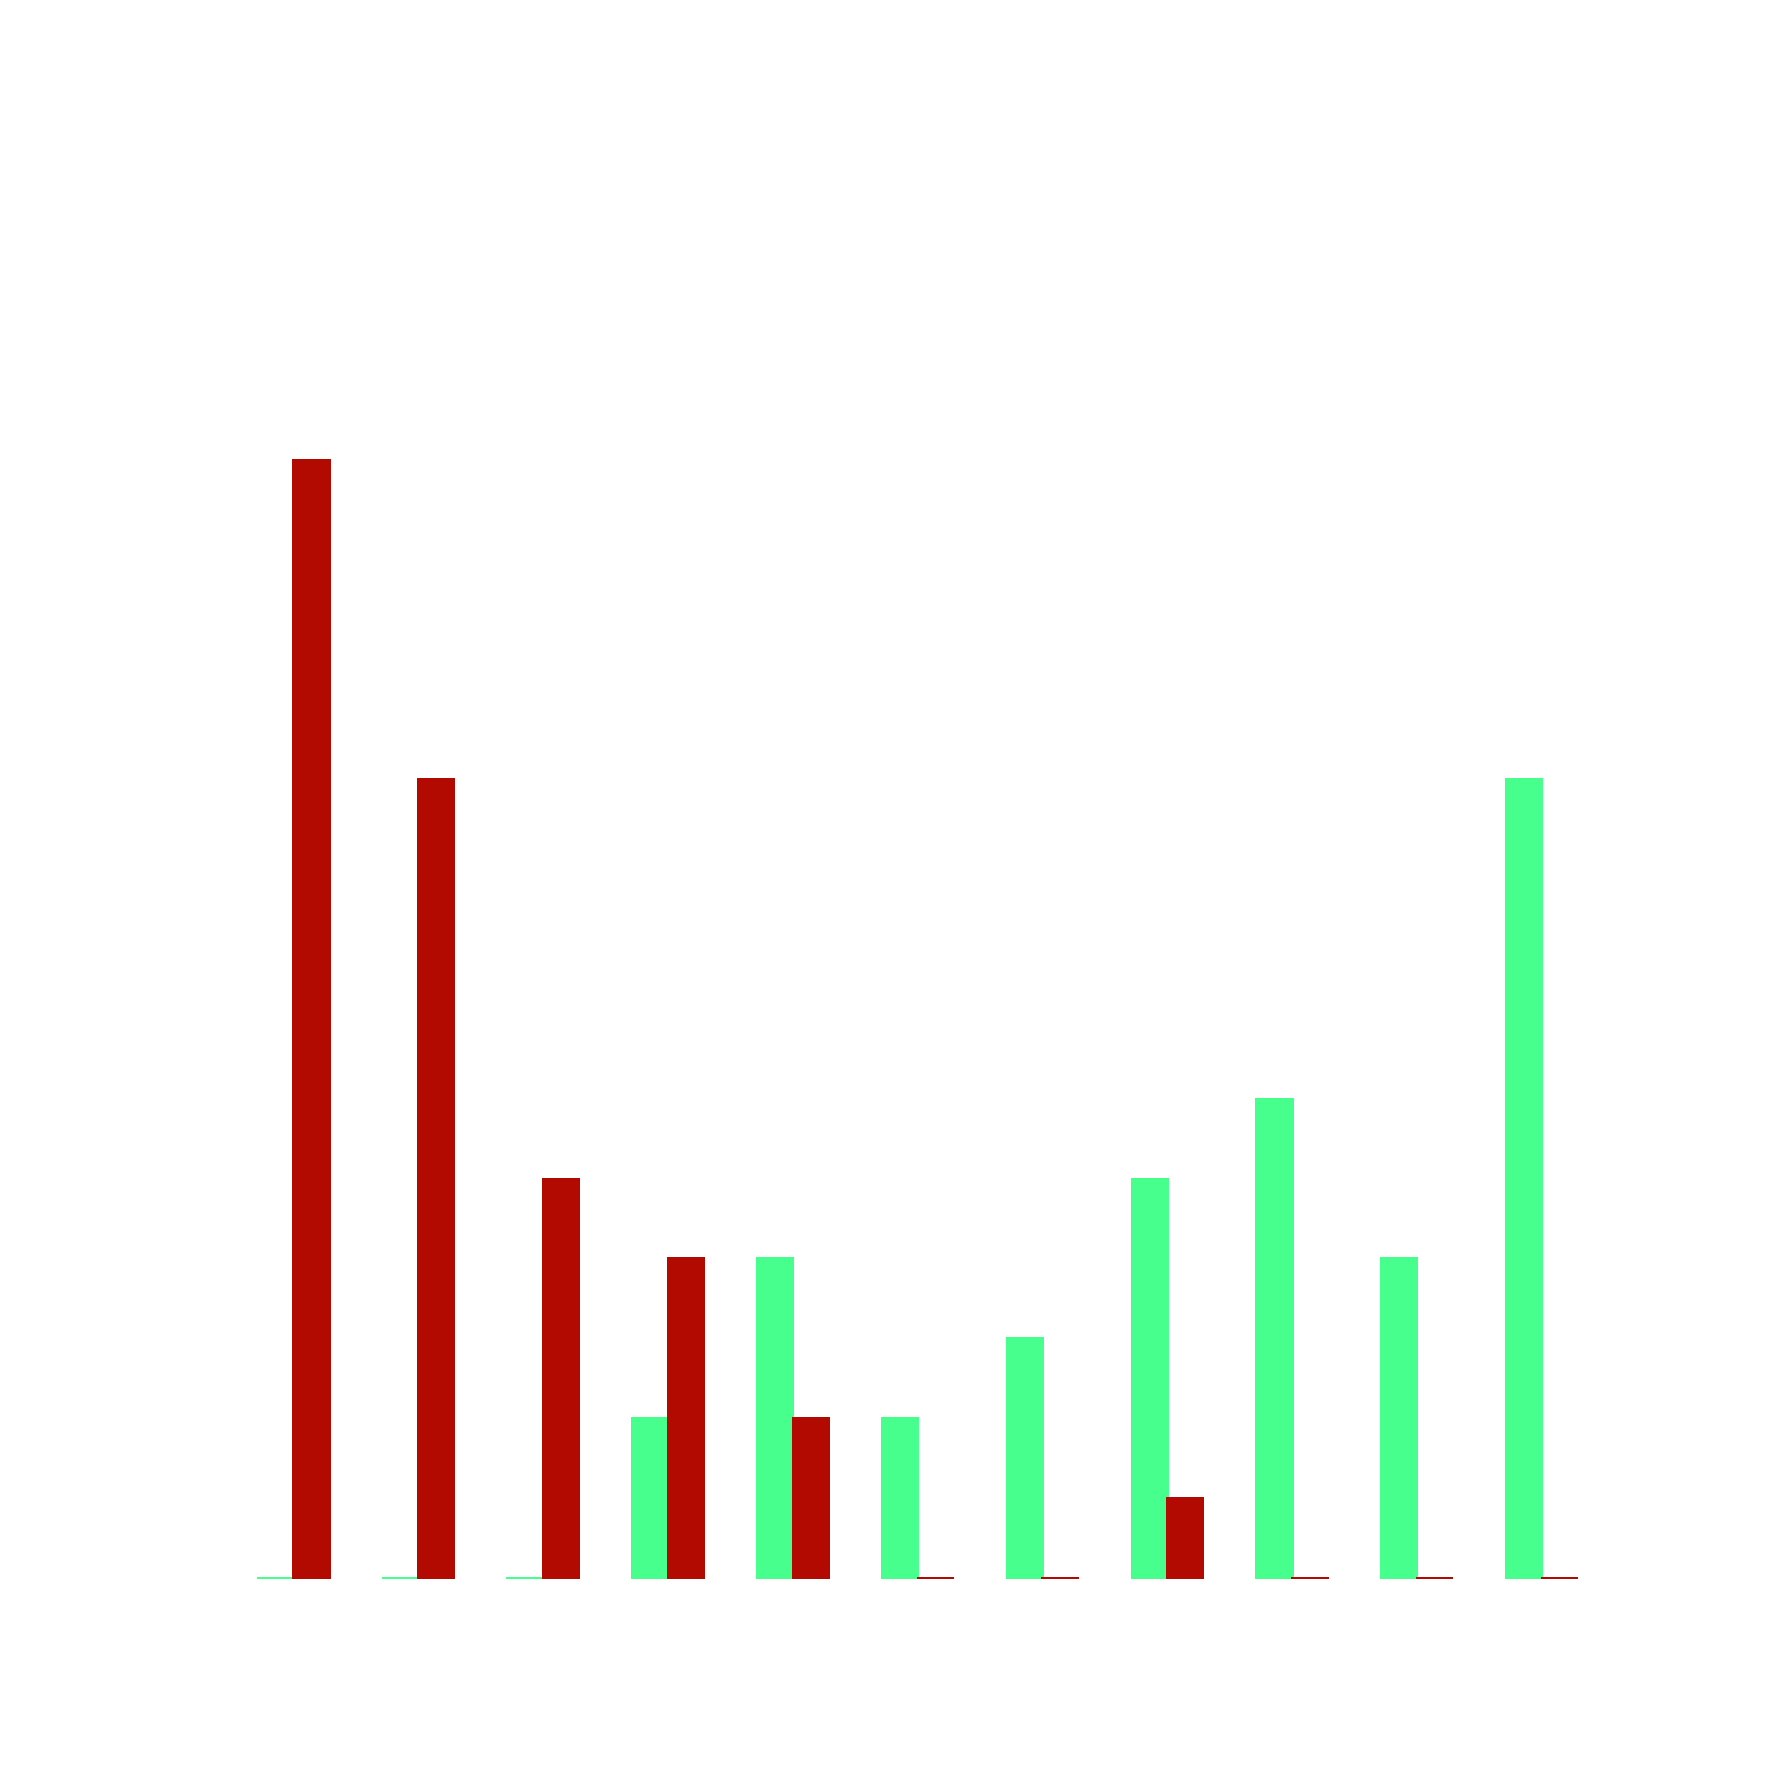
\includegraphics[width=.24\linewidth]{gfx/ch_5/xp4_note_5}\label{fig:xp4_note_1e}}
        \subfloat[sujet 6]
        {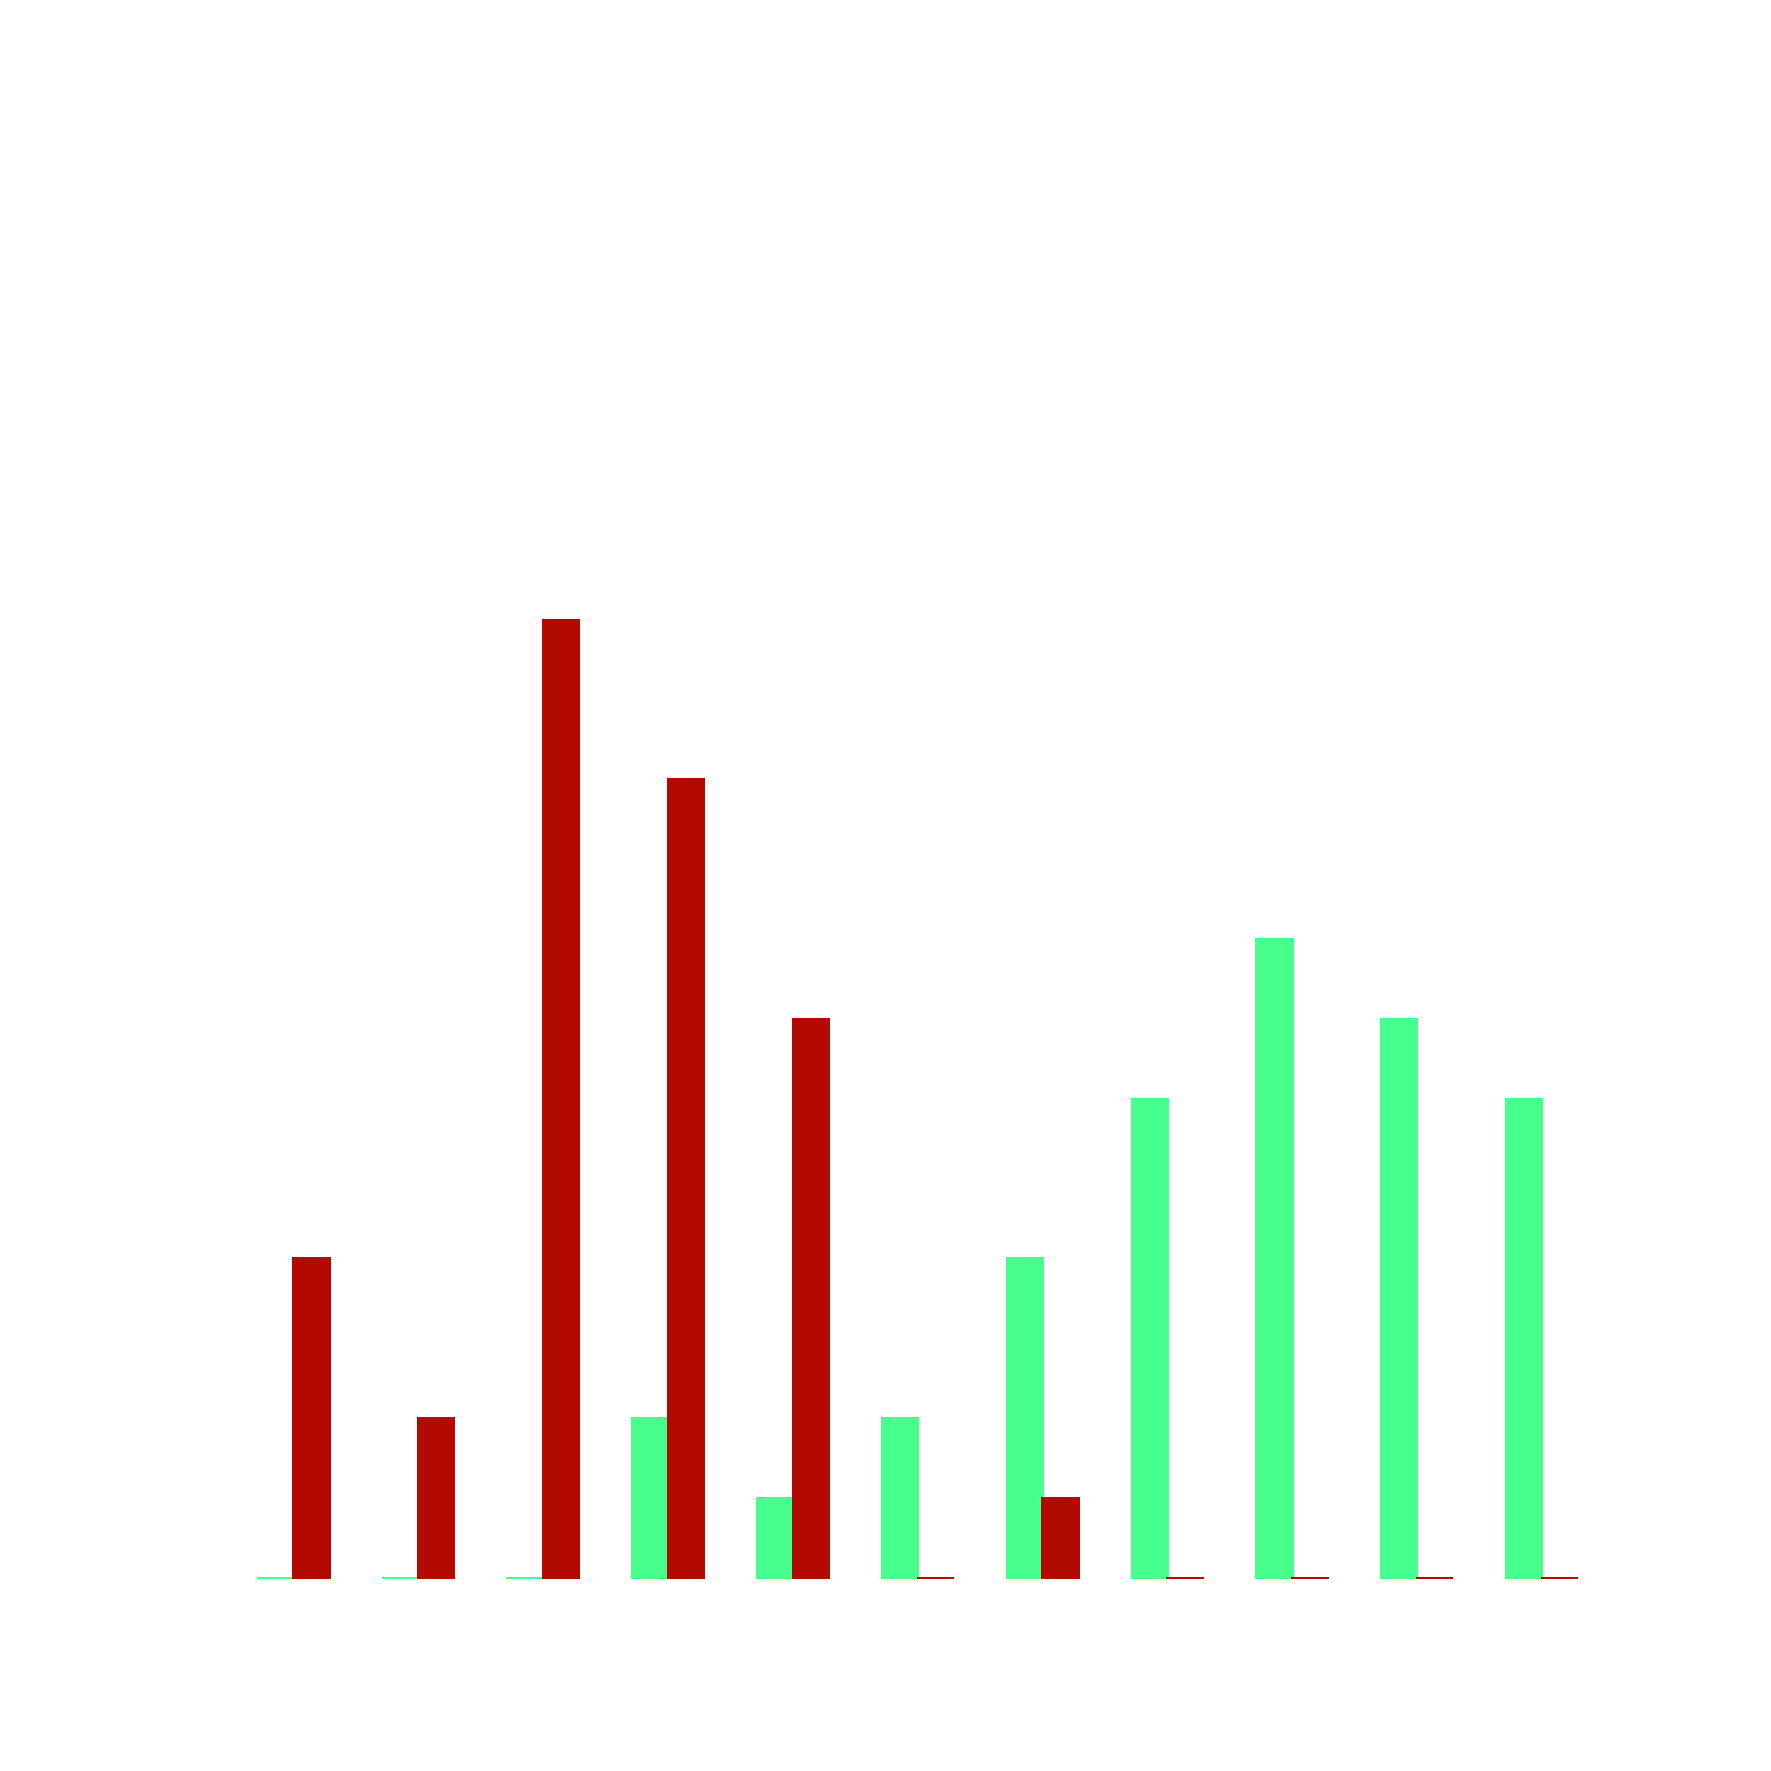
\includegraphics[width=.24\linewidth]{gfx/ch_5/xp4_note_6}\label{fig:xp4_note_1f}}
        \subfloat[sujet 7]
        {\includegraphics[width=.24\linewidth]{gfx/ch_5/xp4_note_7}\label{fig:xp4_note_1g}}
        \subfloat[sujet 8]
        {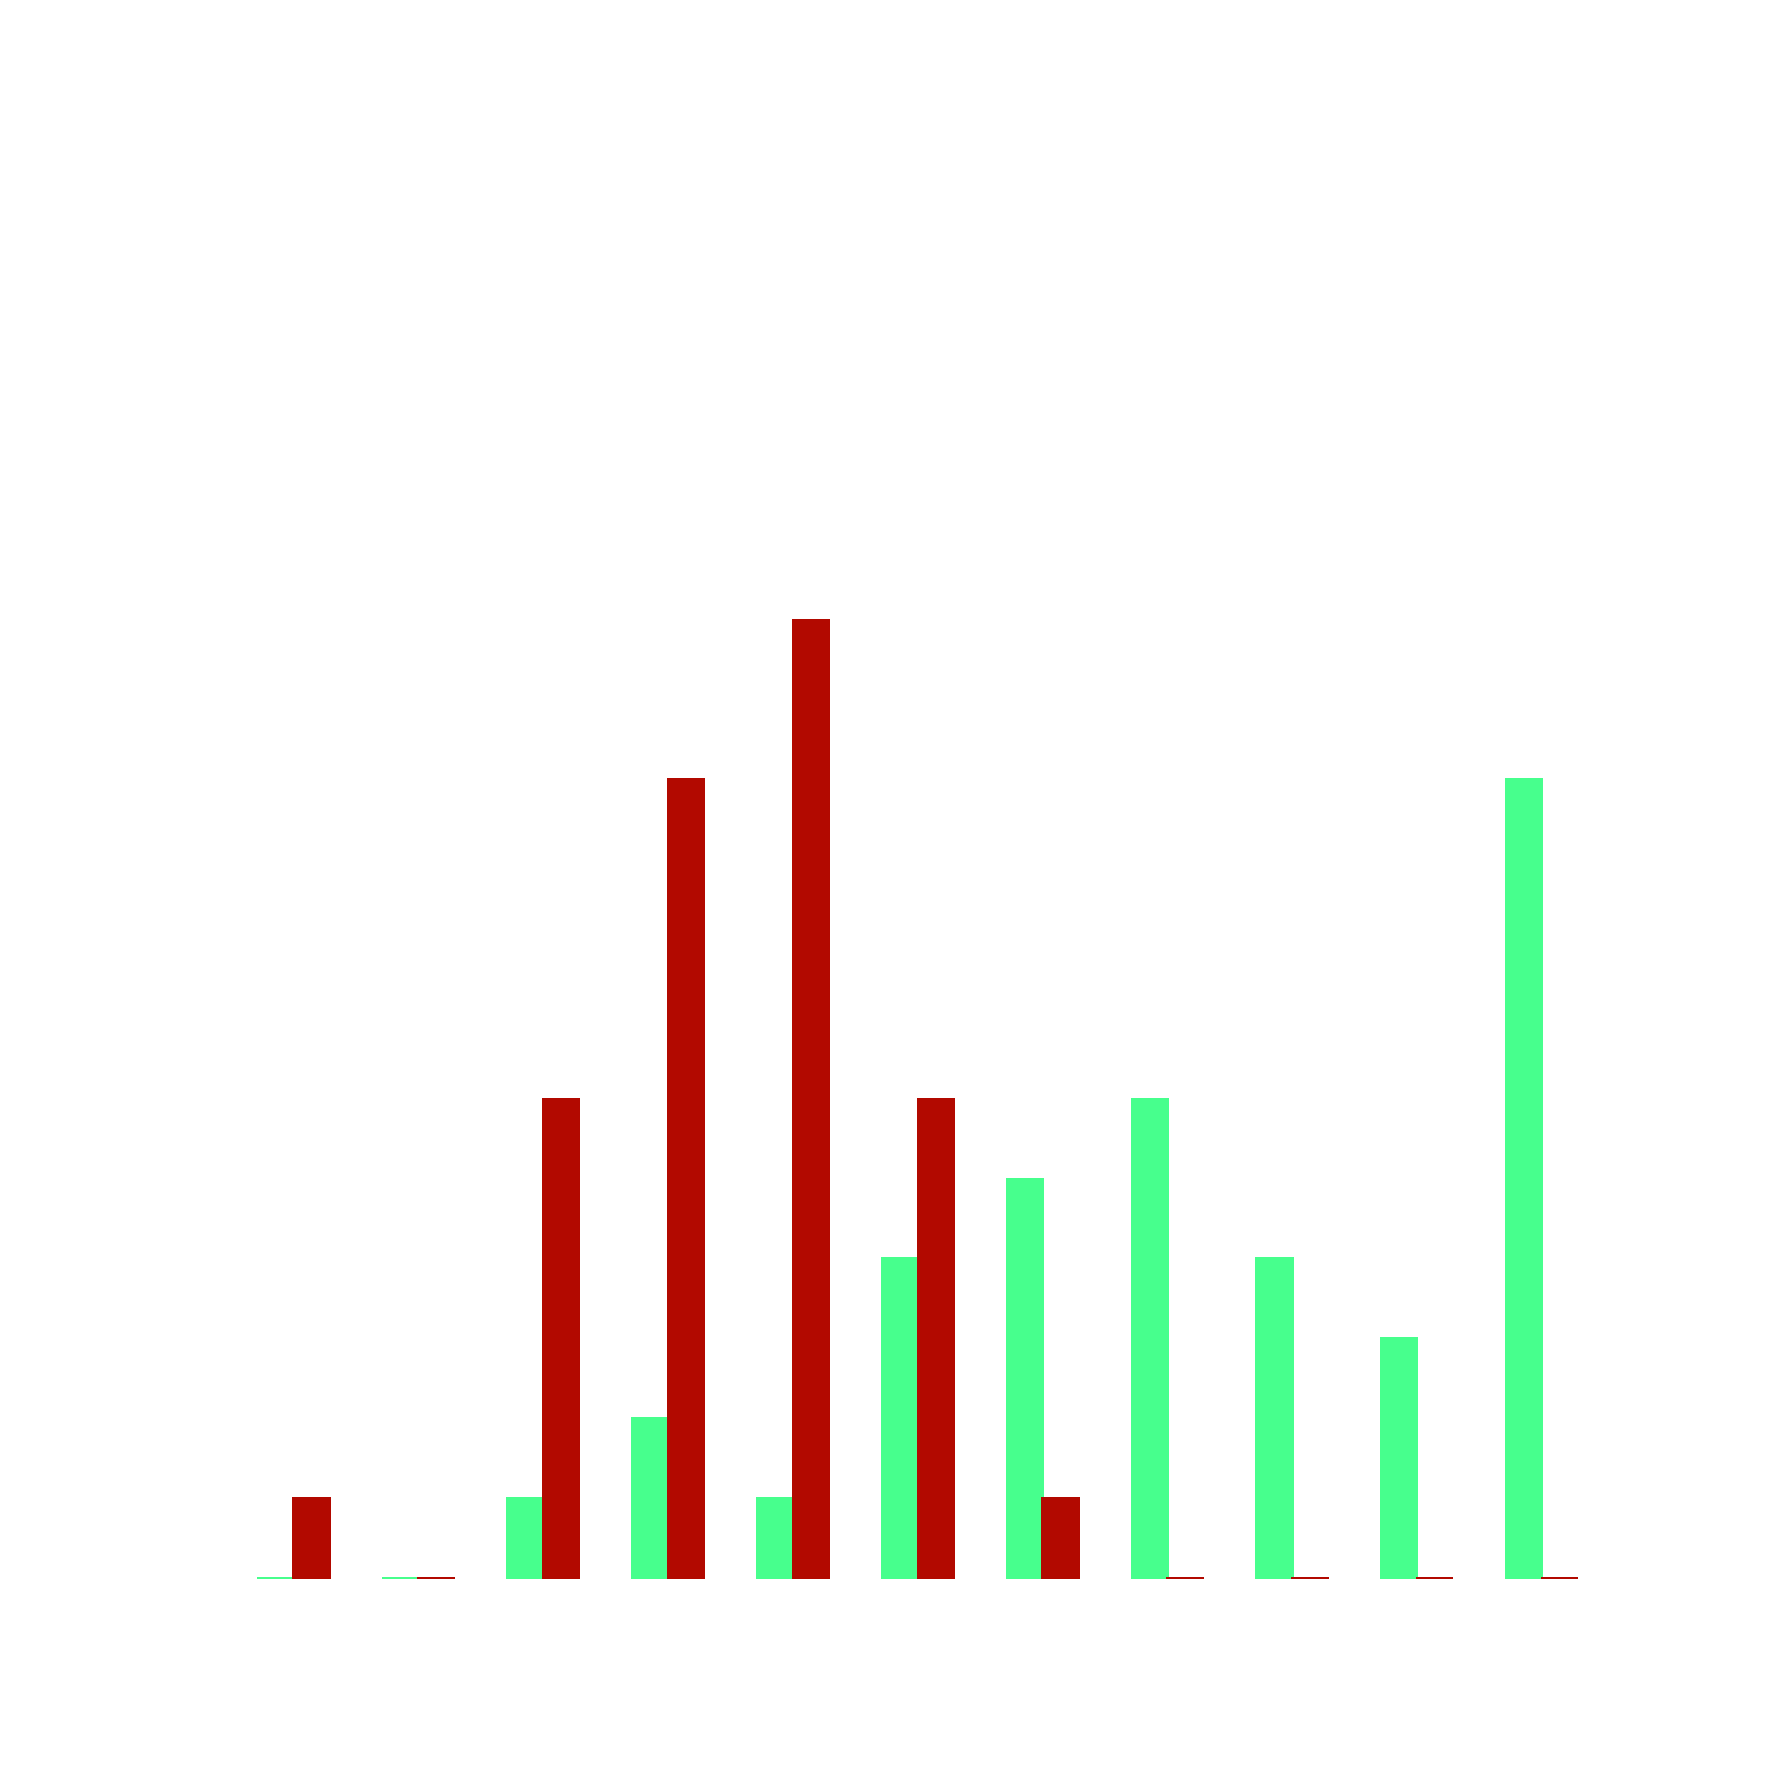
\includegraphics[width=.24\linewidth]{gfx/ch_5/xp4_note_8}\label{fig:xp4_note_1h}} \par
        \subfloat[sujet 9]
        {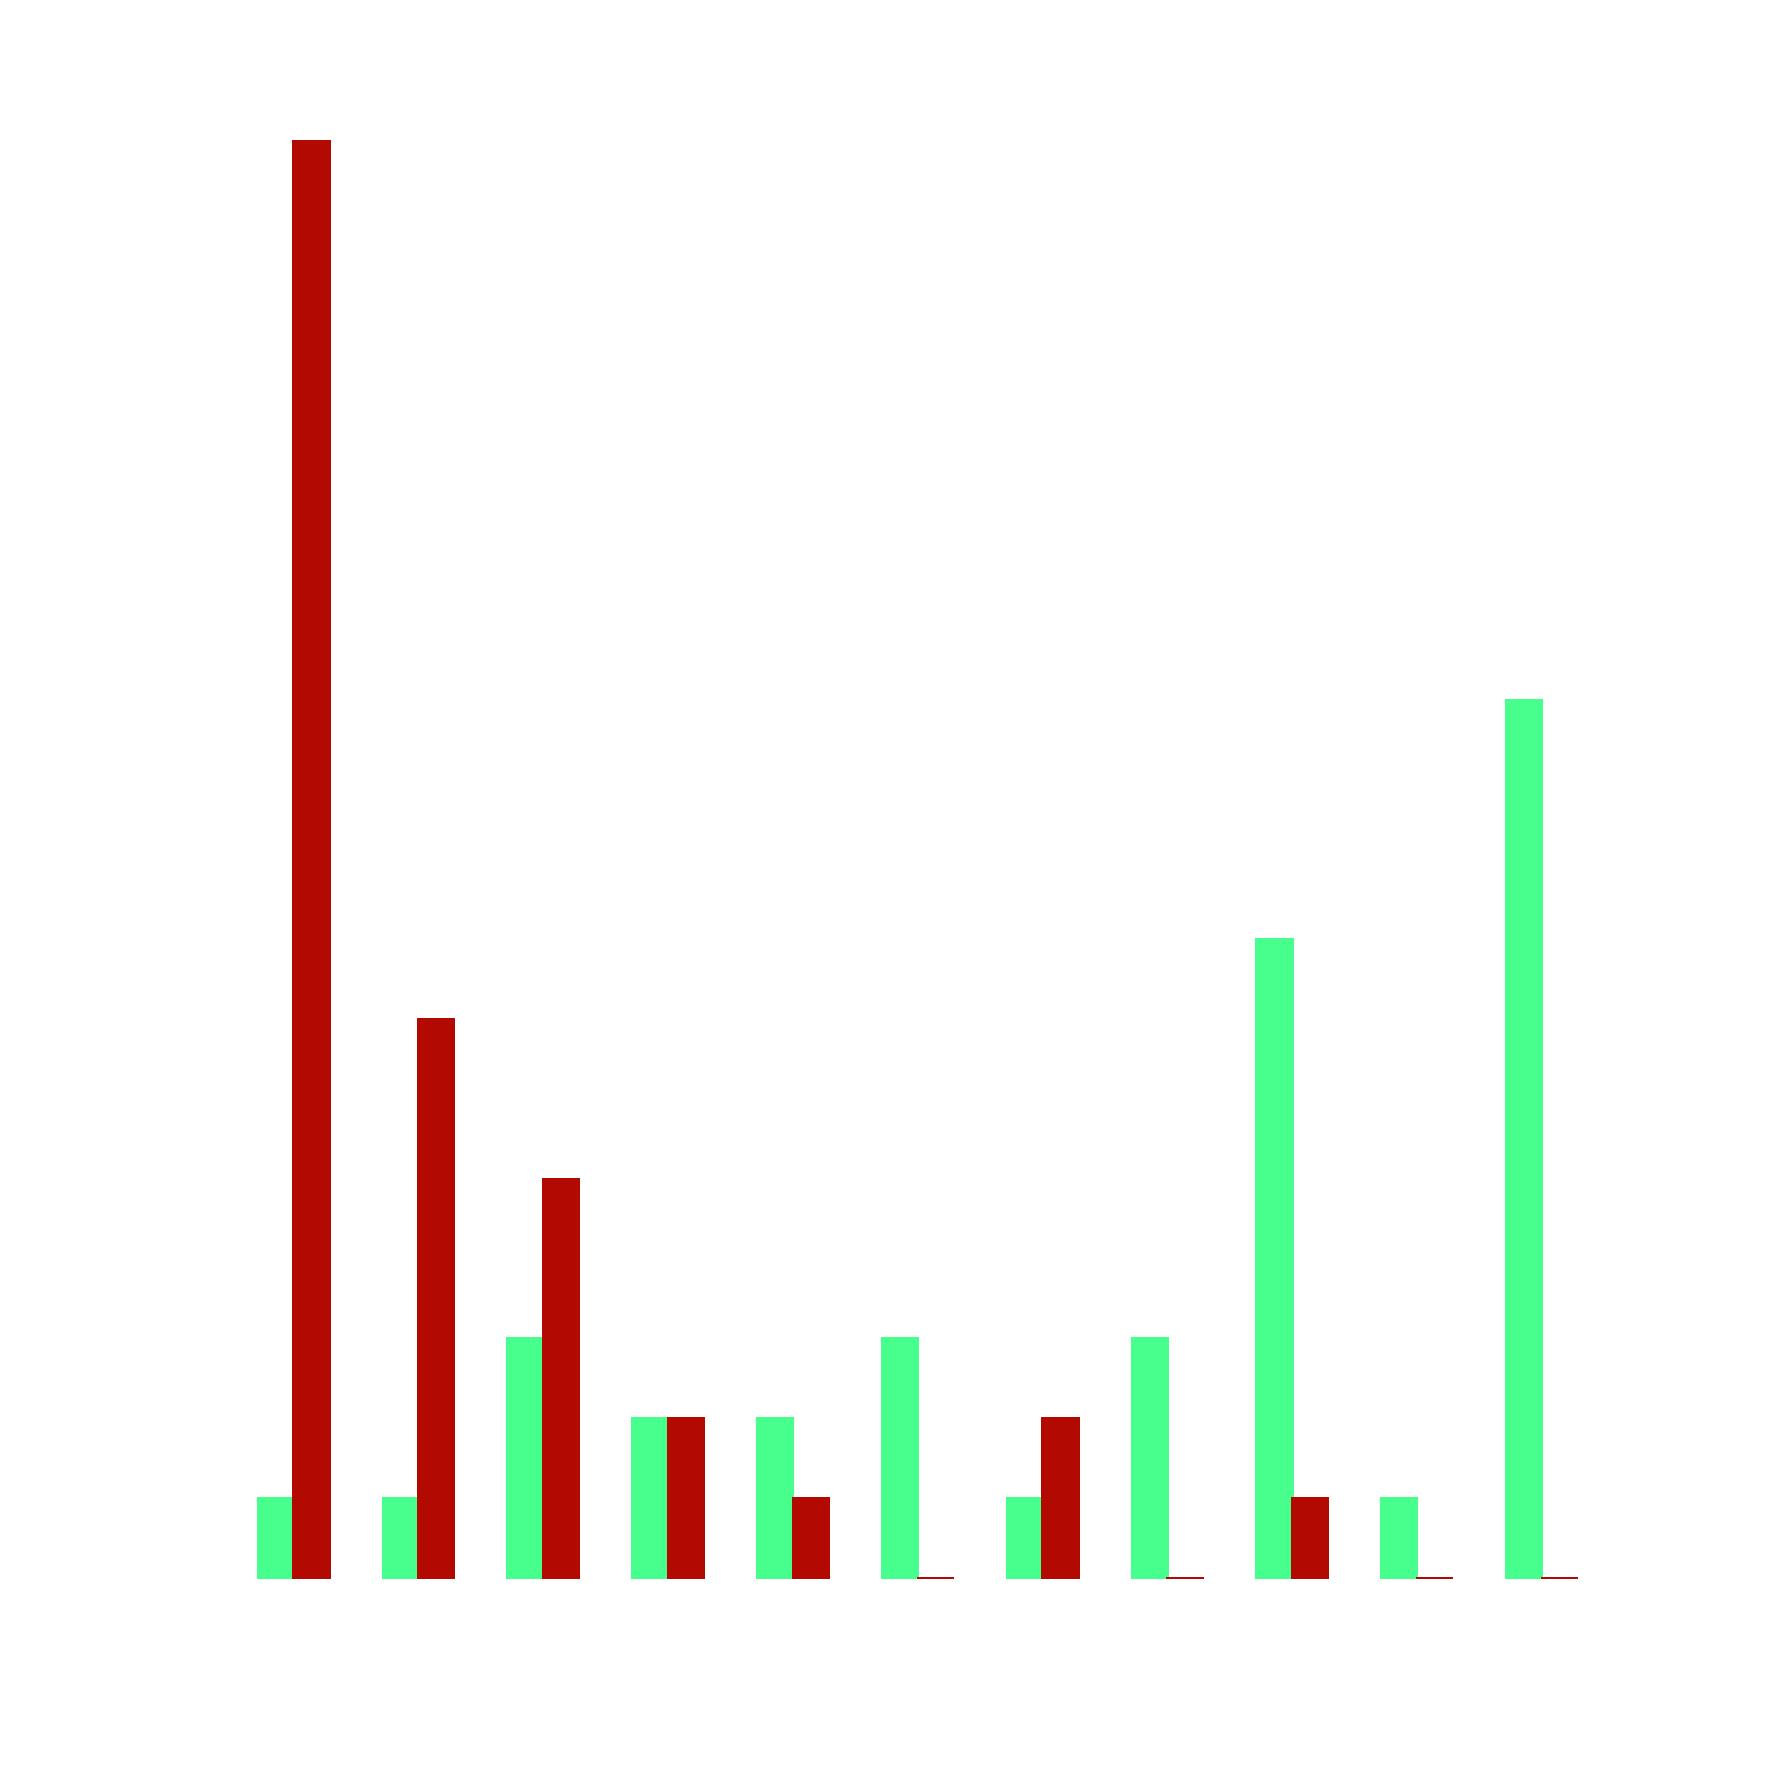
\includegraphics[width=.24\linewidth]{gfx/ch_5/xp4_note_9}\label{fig:xp4_note_1i}}
        \subfloat[sujet 10]
        {\includegraphics[width=.24\linewidth]{gfx/ch_5/xp4_note_10}\label{fig:xp4_note_1j}}
        \subfloat[sujet 11]
        {\includegraphics[width=.24\linewidth]{gfx/ch_5/xp4_note_11}\label{fig:xp4_note_1h}}
        \subfloat[sujet 12]
        {\includegraphics[width=.24\linewidth]{gfx/ch_5/xp4_note_12}\label{fig:xp4_note_1l}}
        \caption{Dispersions des notes données par les sujets lors de l'expérience 2 aux i/am-scènes (vert) et ni/am-scènes (rouge).}\label{fig:xp4_note_1}
\end{figure}

\end{document}
